
%%%%%%%%%%%%%%%%%%%%%%%%%%%%%%%%%%%%%%%%%%%%%%%%%%%%%%%%%%%%%%%%%%%%%%%%
%%
%% main.tex
%% LaTeX-2e 専用
%% 
%% 
%%        設計工学研究室 学位論文テンプレート
%%
%%                      作成日時    2018年 10月 1日
%%
%%%%%%%%%%%%%%%%%%%%%%%%%%%%%%%%%%%%%%%%%%%%%%%%%%%%%%%%%%%%%%%%%%%%%%%%

\documentclass[12pt, a4paper, titlepage, dvipdfmx]{jsbook}      %ドキュメントクラス

%パッケージ
\usepackage[dvipdfmx]{graphicx, color}
\usepackage{amsmath}
\usepackage{amssymb}
\usepackage{array}
\usepackage{hhline}
\usepackage{afterpage}
\usepackage{enumerate}
\usepackage{multicol}
\usepackage{fancyhdr}
\usepackage{subfigure}
\usepackage{bm} %ベクトル表示
\usepackage{slashbox}  % https://qiita.com/ta_b0_/items/2619d5927492edbb5b03
\usepackage{listings, jvlisting}
\usepackage{url}
\usepackage[final,dvipdfmx]{pdfpages}
\usepackage{pgf-umlcd}

%プログラム挿入の設定
\lstset{
	%プログラム言語(複数の言語に対応,C,C++も可)
 	language = C++,
 	%背景色と透過度
 	backgroundcolor={\color[gray]{.90}},
 	%枠外に行った時の自動改行
 	breaklines = true,
 	%自動開業後のインデント量(デフォルトでは20[pt])	
 	breakindent = 10pt,
 	%標準の書体
 	basicstyle = \ttfamily\scriptsize,
 	%basicstyle = {\small}
 	%コメントの書体
 	commentstyle = {\bfseries \color[cmyk]{1,0.4,1,0}},
 	%関数名等の色の設定
 	classoffset = 0,
 	%キーワード(int, ifなど)の書体
 	keywordstyle = {\bfseries \color[cmyk]{0,1,0,0}},
 	%""で囲まれたなどの"文字"の書体
 	stringstyle = {\ttfamily \color[rgb]{0,0,1}},
 	%枠 "t"は上に線を記載, "T"は上に二重線を記載
	%他オプション:leftline,topline,bottomline,lines,single,shadowbox
 	frame = TBrl,
 	%frameまでの間隔(行番号とプログラムの間)
 	framesep = 5pt,
 	%行番号の位置
 	numbers = left,
	%行番号の間隔
 	stepnumber = 1,
	%右マージン
 	%xrightmargin=0zw,
 	%左マージン
	%xleftmargin=3zw,
	%行番号の書体
 	numberstyle = \tiny,
	%タブの大きさ
 	tabsize = 4,
 	%キャプションの場所("tb"ならば上下両方に記載)
 	captionpos = t
}


%新定義コマンド
\newcommand{\sankou}[1]{$ ^{\text{[#1]}} $}
\newcommand{\chref}[1]{第~\ref{#1}~章}
\newcommand{\secref}[1]{\ref{#1} (p.\pageref{#1})}
\newcommand{\tableref}[1]{Table.\ref{#1}}
\newcommand{\figref}[1]{Fig.\ref{#1}}
\newcommand{\figpref}[1]{(Fig.\ref{#1} p.\pageref{#1})}
\newcommand{\degree}{\char'27\kern-.3em\hbox{C}} 

%再定義コマンド
\renewcommand{\figurename}{Fig.~}
\renewcommand{\tablename}{Table.~}
\renewcommand{\labelitemi}{・}
\renewcommand{\labelenumi}{(\theenumi)}

\renewcommand{\eqref}[1]{式 (\ref{#1})}

\renewcommand{\subfigtopskip}{0mm}%図と図の間
\renewcommand{\subfigcapskip}{0mm}%図と副題の間

%余白変更
\setlength{\textwidth}{\fullwidth}
\setlength{\evensidemargin}{\oddsidemargin}

\title{学位論文のテンプレート}
\author{埼玉大学 工学部 機械工学科
        \\
        埼玉 太郎
        }

\begin{document}

    %タイトル
    %%%%%%%%%%%%%%%%%%%%%%%%%%%%%%%%%%%%%%%%%%%%%%%%%%%%%%%%%%%%%%%%%%%%%%%%
%%
%% 題目.tex
%% LaTeX-2e 専用
%% 
%% 
%%        設計工学研究室 学位論文テンプレート
%%
%%                      作成日時    2020年 2月 11日
%%
%%%%%%%%%%%%%%%%%%%%%%%%%%%%%%%%%%%%%%%%%%%%%%%%%%%%%%%%%%%%%%%%%%%%%%%%
\thispagestyle{empty}
\newcommand{\ctext}[1]{\textcolor[rgb]{0.65, 0.65, 0.65}{\raise0.2ex\hbox{\textcircled{\scriptsize{#1}}}}}
%% 卒業論文題目     
\begin{center}
        {\huge 埼玉大学 工学部} \\
        {\huge 機械工学科} \\        
        \vspace{10mm}
        {\Huge 令和5年度 \quad 卒業論文}\\
        \vspace{10mm} 
        
        {\Huge ○○○○○○○○○○の研究} \\
        \vspace{10mm}
        {\LARGE Study on XXXXXXXXXX} \\        
        \vspace{35mm} %題目の長さに応じて適宜修正すること
 \end{center}
        
 \begin{table}[!h]
        \begin{flushright}        
        \renewcommand{\arraystretch}{1.5}
        \begin{tabular}{|c|cc|}
            \hline
            {\Large 学科長}    & {\Large  荒居善雄 教授 \quad} & {\Large\ctext{印}}\\        
            \hline
            {\Large 主指導教員} & {\Large  琴坂信哉 准教授 } &{\Large\ctext{印}}\\
            \hline
            {\Large 副指導教員} & {\Large  程島竜一 准教授 }& \\
            \hline
        \end{tabular}
        \renewcommand{\arraystretch}{1.0}        
    \end{flushright}        
 \end{table}
\begin{table}[!b]
        \begin{flushright}
        \renewcommand{\arraystretch}{1.2}
        \begin{tabular}{|c|c|}
            \hline
             {\Large 提出日} & {\Large 2023年2月XX日}\\ %年は西暦で記載
             \hline
             {\Large 研究室} & {\Large 設計工学 }\\
             \hline
             {\Large 学籍番号} & {\Large 20TM028}\\
             \hline
             {\Large 氏  名} & {\Large 長谷川 大晴}\\
            \hline
        \end{tabular}
        \renewcommand{\arraystretch}{1.0}
        \end{flushright}
\end{table}
                                %タイトル ※修士は題目_修士、学士は題目_学士に変更すること。編集するファイルもそれぞれ対応するファイルを編集する。

    \frontmatter
    \tableofcontents
    \listoffigures
    \listoftables
    \mainmatter{} 
    %!!重要!!
    %各章は奇数ページから開始するように調整すること
    %つまり各章は偶数ページで終わるように、改ページ等を使用して調整する。
    
\chapter{序論}\label{chapter:序論}
第\ref{chapter:序論}章では,本研究の背景と先行研究,そして研究の目的を述べる.


\section{背景}

% 流れ
% 多脚ロボットの特徴と,不整地の移動に適していることを述べる
% 不整地の移動において,6脚であることによる利点を述べる
% 適応歩容の必要性を述べる
% 適応歩容の実現方法を述べる,そして,グラフ探索による手法を述べる

% 1.1.1 章
\subsection{不整地における多脚ロボットの活用}
近年,人間に代わって作業を行う移動ロボットの導入が進められている\cite{Sotnik_Prospects_for_Introduction}.
Pudu社が開発したロボットのBellaBot\cite{Pudu_BellaBot}が,
レストランで配膳の作業を行う姿は一般に見ることができるようになった.
これらのロボットは人間が移動を行う空間での使用を前提としており,
多くはタイヤやクローラを用いて移動を行うが,
その他の移動様式を用いるロボットとして,
脚を使用して移動を行うロボット(以下脚ロボット)が存在する.
文献\cite{Locomotion_for_difficult_terrain}では脚ロボットは他の移動様式を用いて移動するロボットに比べて,
以下に示すような利点があると述べられている.

\begin{itemize}
  \item 障害物をまたいで移動できるため,対地適応性が高い
  \item 脚接地点を離散的に選択できるため,環境に与える影響が小さい
  \item スリップすることなく全方向に移動できる
\end{itemize}

障害物をまたいで移動できることにより,
脚ロボットはタイヤでは移動できないような凹凸が激しい地形や,
不連続な地形においても移動することが可能である.
また,砂利で舗装された道のような,
クローラではスリップしてしまうような環境においても移動することが可能である.
この特徴を生かして,
実際に\figref{fig:nedo_spot}のようにBoston Dynamics Inc. によって開発された
4足歩行ロボットのSpot\cite{Boston_Dynamics_Spot}を用いて,
林業を行う山間地で作業を行う実証実験が行われている\cite{NEDO}.
山間地は斜面である上に,伐根作業によって木の根が残っているため凹凸が激しく,
タイヤやクローラでは移動が困難である.
しかし,脚ロボットであるSpotは障害物をまたいで移動することができるため,
このような環境での作業に適しており,
導入による人手不足の解消や,作業効率の向上が期待されている.

また,離散的に脚接地地点を選択できるため,
タイヤやクローラによる移動と比較して環境に与える影響が小さい.
この特徴を生かしたロボットの実例として,
韓国海洋科学技術院によって開発された6脚ロボットのCrabster\cite{J_Kim_Dexterous_Crabster}があげられる.
\figref{fig:crabster}に示したCrabsterは,流れの早い海底での作業を想定して開発されており,
6本の脚による移動を行うことや,4本の脚を海底に接地させ,
残りの2本の脚を用いて作業を行うことが可能である.
脚を用いた移動では海底の砂を大量に巻き上げることがないため\cite{J_Kim_Little_Crabster},
カメラを用いた観察や,センサを用いた地形の計測に優れている.
以上より,脚ロボットは対地適応性が高く,環境に与える影響が小さいため,
不整地での移動に適しているといえる.

\begin{figure}[htbp]
  \begin{center}
    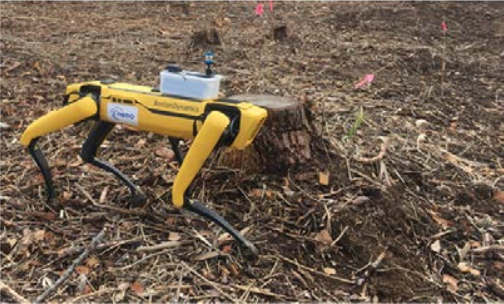
\includegraphics[width=90mm, clip]{figure/chapter1/NEDO.png}
    \caption{Demonstration Experiment with Spot}
    \label{fig:nedo_spot} % chktex 24
  \end{center}
\end{figure}

\begin{figure}[htbp]
  \begin{center}
    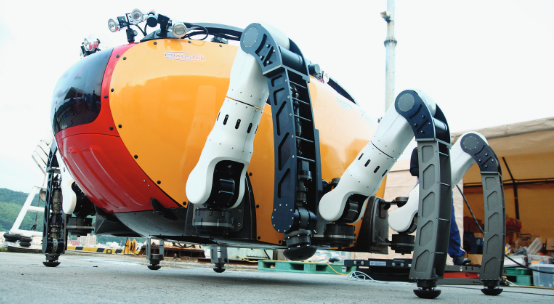
\includegraphics[width=90mm, clip]{figure/chapter1/crabster.png}
    \caption{Crabster}
    \label{fig:crabster} % chktex 24
  \end{center}
\end{figure}

このような特徴をもつ脚ロボットであるが,実際に不整地で活用された事例は多くない.
原因として,\cite{Locomotion_for_difficult_terrain}では
以下に示すような問題を脚ロボットが抱えているためと述べられている.

\begin{itemize}
  \item 脚の機構はアクチュエータの数が多いため,重量が大きくなってしまう
  \item 移動には歩行のための制御が必要であり,タイヤやクローラに比べて制御が複雑になる
\end{itemize}

多脚ロボットの積極的な活用を考えると,脚の機構の軽量化と,
歩行のための制御の手法が必要である.
そこで本研究では多脚ロボットの制御に着目し,
不整地における多脚ロボットの活用のための歩行の制御手法を論じることとする.

不整地で脚ロボットを歩行させることを前提に,脚ロボットの歩行形態について考える.
脚ロボットの歩行形態は大別して,動歩行と静歩行に分けられる.
静歩行とは,支持脚多角形とも呼ばれる,
地面に接地している脚をすべて結んでできる多角形上に重心をおき,
常に静的な安定性を保ちながら歩行することと定義される\cite{Hirose_Static_stability_criterion}.
それに対して動歩行とは静的には不安定であるが,動的に安定を保ちながら歩行することである.
静歩行では常に支持脚多角形上に重心を置くため,動歩行と比較して歩行速度が遅くなる.
しかし,動歩行は重心の位置や歩行の速度を踏まえた動的な制御が必要となるため,静歩行に比べて制御が複雑になる.
加えて不整地の歩行では地形の状態を考慮する必要があるため,より制御の難易度は高くなる.
そのため,静歩行を用いたほうが不整地歩行を実現しやすいことがわかる.

静歩行による不整地の歩行は,主に4脚以上の脚ロボットで研究されている.
なぜならば,2脚を有する脚ロボットは静的な安定性を保ちながら歩行する場合,
重心の位置が支持脚面積の中になるように制御する必要があるため,
実用的な歩行速度を得ることが難しいためである.
そのため,より早い静歩行には4脚以上の脚を有する脚ロボットが有利である.
本論文ではそのような4,6脚以上の脚を有する脚ロボットを多脚ロボットと呼ぶことにする.

先述した問題点から,多脚ロボットの脚数は少ないほうが望ましい.
実際に多くの研究において,静歩行が可能な最小の脚数を有する4脚ロボットや6脚ロボットが用いられている.

% 1.1.2 章
\subsection{固定歩容と自由歩容}
多脚ロボットが歩行を行う際には,脚を適切な順番で動かす必要がある.
脚ロボットの歩行中の脚を動かす順序や,脚を動かすタイミングのことを歩容と呼ぶ.
歩容にはさまざまな種類があるが,大別すると周期的に同じパターンの脚の動作を繰り返す固定歩容と,非周期的に脚を動かす自由歩容に分けられる.

固定歩容は自然界においても多く見られる歩容であり,動物の歩行や,昆虫の歩行などがこれにあたる.
代表的なものとしては,低速で4足歩行をする動物にみられるクロール歩容がある.
これは,歩行中に常に3本の脚が地面に接地しており,1本の脚が遊脚する歩容パターンである.
3本の脚が地面に接地しているため,常に静的な安定性を保つことができるが,1本づつしか脚を動かせないため,一般に歩行速度は遅い.

6足歩行する昆虫の中には,トライポッド歩容と呼ばれる歩容をとるものがある.
この歩容パターンでは,まず片側の前脚と後ろ脚,反対側の中央の脚を地面に接地させ,残りの3本の脚を遊脚させる.
次に,反対側の前脚と後ろ脚,片側の中央の脚を地面に接地させ,残りの3本の脚を遊脚させる動作を繰り返す.
この歩容では同時に3本の脚を地面に接地させることができるため,クロール歩容よりも歩行速度が速くなる.

固定歩容は平地において比較的高速かつ安定した歩行を実現することができるが,
不整地においては遊脚の可動範囲内の接地点が存在しない場合,歩容を維持することができない.
多脚ロボットの対地適応性を生かすためには,地形に応じた自由歩容パターンを生成する必要があるといえる.

% 1.1.3 章
\subsection{グラフ探索による自由歩容パターン生成手法}
自由歩容パターンを生成する手法として,グラフ探索による自由歩容パターン生成手法がある\cite{Prabir_Graph_search}.
これは,脚位置や動作を離散化することでロボットの歩容をグラフに落としこみ,
そのグラフを探索することによって数動作先までの歩容パターンの組み合わせを網羅的に調べ,最適な歩容パターンを選択する手法である.
この手法の特徴として,数動作先までを考慮して歩容パターンを生成するため,デッドロックに陥りにくいという点や,
効率的な歩容パターンを生成することができるという点が挙げられる.

しかし,グラフ探索による自由歩容パターン生成手法は,脚の本数が増えることで脚の動かし方の組み合わせが増えるため,
グラフの規模が大きくなり,実時間内の計算が困難になるという問題がある.
4脚ロボットにおいて,静的安定性を保ちながら歩行する場合,1度に遊脚することができる脚は1本であるため,
実時間内の計算は容易である.
だが,6脚ロボットは静的安定性を保ちながら最大3本の脚を遊脚することができるため,
グラフの規模が大きくなり,実時間内の計算が困難になる.
この問題を解決するためにPrabirらは歩容をウェーブ歩容に限定することで,
グラフの規模を小さくすることに成功した\cite{Prabir_Graph_search_Six},
また新らは歩容をトライポッド歩容に限定することで\cite{Arata_Graph_search_Six},
同様にグラフの規模を小さくしている.
これらの手法は歩容を限定することでグラフの規模を小さくすることに成功しているが,
ロボットの行う動作の種類が限定されてしまうという問題がある.

そこで本研究室ではロボットの動作を制限することなく,グラフ探索による自由歩容パターン生成手法を6脚ロボットに適用するため,
離散化された脚位置の組み合わせを利用してグラフの階層構造化を行った.
また,自由歩容パターン生成による接地地点の計算と脚軌道の生成を分離した.
これらによって,グラフ探索による自由歩容パターン生成手法を6脚ロボットに適用することが可能になった.

本研究室では,ロボットを動作させる地形やロボットの動作によって段階的に開発を行っており,
これまでに2次元空間において,直進動作\cite{Oki_Graph_search},目的姿勢での停止\cite{Nakaoka_Graph_search},
旋回動作\cite{Shina_Graph_search}を行うための歩容パターン生成手法の実装に成功した.
また3次元空間においても,脚位置の離散化方法を3次元に適応させたことで\cite{Miura_Graph_search},
直進動作\cite{Hato_Graph_search}を行うための歩容パターン生成手法の実装に成功した.

\section{本研究の目的}
これまでの研究によって,3次元の不整地において,重心高さを変更しつつ,
自由歩容パターン生成を行うことが可能となった.
しかし低頻度ではあるが,グラフ探索に成功したとしても脚軌道が生成できず,その歩容パターン通りに歩行することできなくなり,
動作を停止してしまう問題が生じてしまった.

これは,グラフ探索と脚軌道生成を分離したことによって生じた問題であり,
先行研究では継続的にこの問題について言及されていたが,
グラフの規模を大幅に増大させることなく,また歩容生成の成功率を低下させることなく,
この問題を解決することはできなかった.

そこで本論文では,常に脚軌道生成に成功するような歩容パターン生成手法を提案し,
脚軌道生成の失敗による動作停止を防ぐことを目的とする.

\section{本論文の構成}
本論文は,全6章から構成される.

第2章「歩容パターンの再評価手法の提案」では,常に脚軌道生成が可能になる手法として,
歩容パターンの再評価手法を提案し,その機能を述べる.

第3章「歩容パターンの再評価手法の実装」では,提案したプログラムの実装方法を述べる.

第4章「再評価手法の有効性の確認のための歩行シミュレーション」では,
提案手法を用いたシミュレーション実験の結果を述べる.

第5章「常に脚軌道生成が可能な自由歩容パターン生成手法を用いた実機による歩行実験」
では,提案手法を用いた実機試験の結果を述べる.

第6章「結論」では本論文の結論と今後の課題を述べる.
 % 第1章
    %% 歩容パターンの再評価手法の提案.tex
%% LaTeX-2e 専用

%% 全体の流れとしては,まず,先行研究の問題点を指摘し,次に,歩容パターンの再評価手法を提案する.

\chapter{歩容パターンの再評価手法の提案}\label{chapter:歩容パターンの再評価手法の提案}
第\ref{chapter:歩容パターンの再評価手法の提案}章では,先行研究の手法およびその問題点を指摘し,
常に脚軌道生成が可能な自由歩容パターン生成手法として,歩容パターンの再評価手法を述べる.

% 先行研究の章
\section{本研究室における自由歩容パターン生成の先行研究}
最初にグラフ探索よる自由歩容パターン生成手法において用いる用語を定義し,
先行研究で行われてきた自由歩容パターン生成手法について述べる.
また,先行研究で用いられてきた自由歩容パターン生成手法の問題点について述べる.

\subsection{グラフ理論について}
本論文ではグラフ理論を用いた自由歩容パターン生成手法を論ずるため,まずはグラフ理論について説明をする.
グラフとは,頂点(ノード)とそれらを結ぶ辺(エッジ)からなる図形である.
このグラフを用いて,さまざまな問題を取り扱う学問をグラフ理論という.

以降の説明を簡単にするため,この論文で用いるグラフ理論の用語について簡潔に述べる.
グラフ上のあるノードから別のノードにエッジを用いて移動することを遷移と呼ぶ.
遷移の際,移動前のノードを始点,移動後のノードを終点と呼ぶ.
グラフの種類は大別して有向グラフと無向グラフに分けられ,
エッジに向きがあるものを有向グラフ(\figref{fig:directed_graph}),
逆に向きを持たないものを無向グラフ(\figref{fig:undirected_graph})という.
また,閉路を持たず,かつ,すべてのノード間にエッジが存在するグラフを木という.
このような木構造をもつグラフのうち,\figref{fig:tree_graph}のように,
根となるノードを持ち,そのノードからすべてのノードに到達可能なものを根付き木という.
根付き木を図形として表現する場合は簡単のため,
\figref{fig:tree_graph}のように根を上部に配置することが多い.

根付き木には無向グラフと有向グラフの2種類が存在するが,
後述する歩行パターングラフは有効グラフであるため,
有向の根付き木について説明を行う.
根付き木のエッジが,根が始点となるように伸びている場合,
あるノードから遷移可能なノードをそのノードの子ノードと呼ぶ.
逆に,あるノードに遷移可能なノードをそのノードの親ノードと呼ぶ.
親ノードを持たないノードを根ノードと呼び,子ノードを持たないノードを葉ノードと呼ぶ.
また,あるノードから根ノードまでのエッジの数をそのノードの深さと呼び,
根ノード自身の深さは0となる.

たとえば\figref{fig:tree_graph}において,ノードAが根ノードであり,ノードB,Cがその子ノードである.
また,ノードB,ノードD,E,ノードCはノードFを子ノードとして持ち,ノードD,E,Fは葉ノードである.
ノードAの深さは0であり,ノードB,Cの深さは1,ノードD,E,Fの深さは2となる.

\begin{figure}[h]
  \subfigure[Undirected Graph]{%
  \label{fig:undirected_graph}
  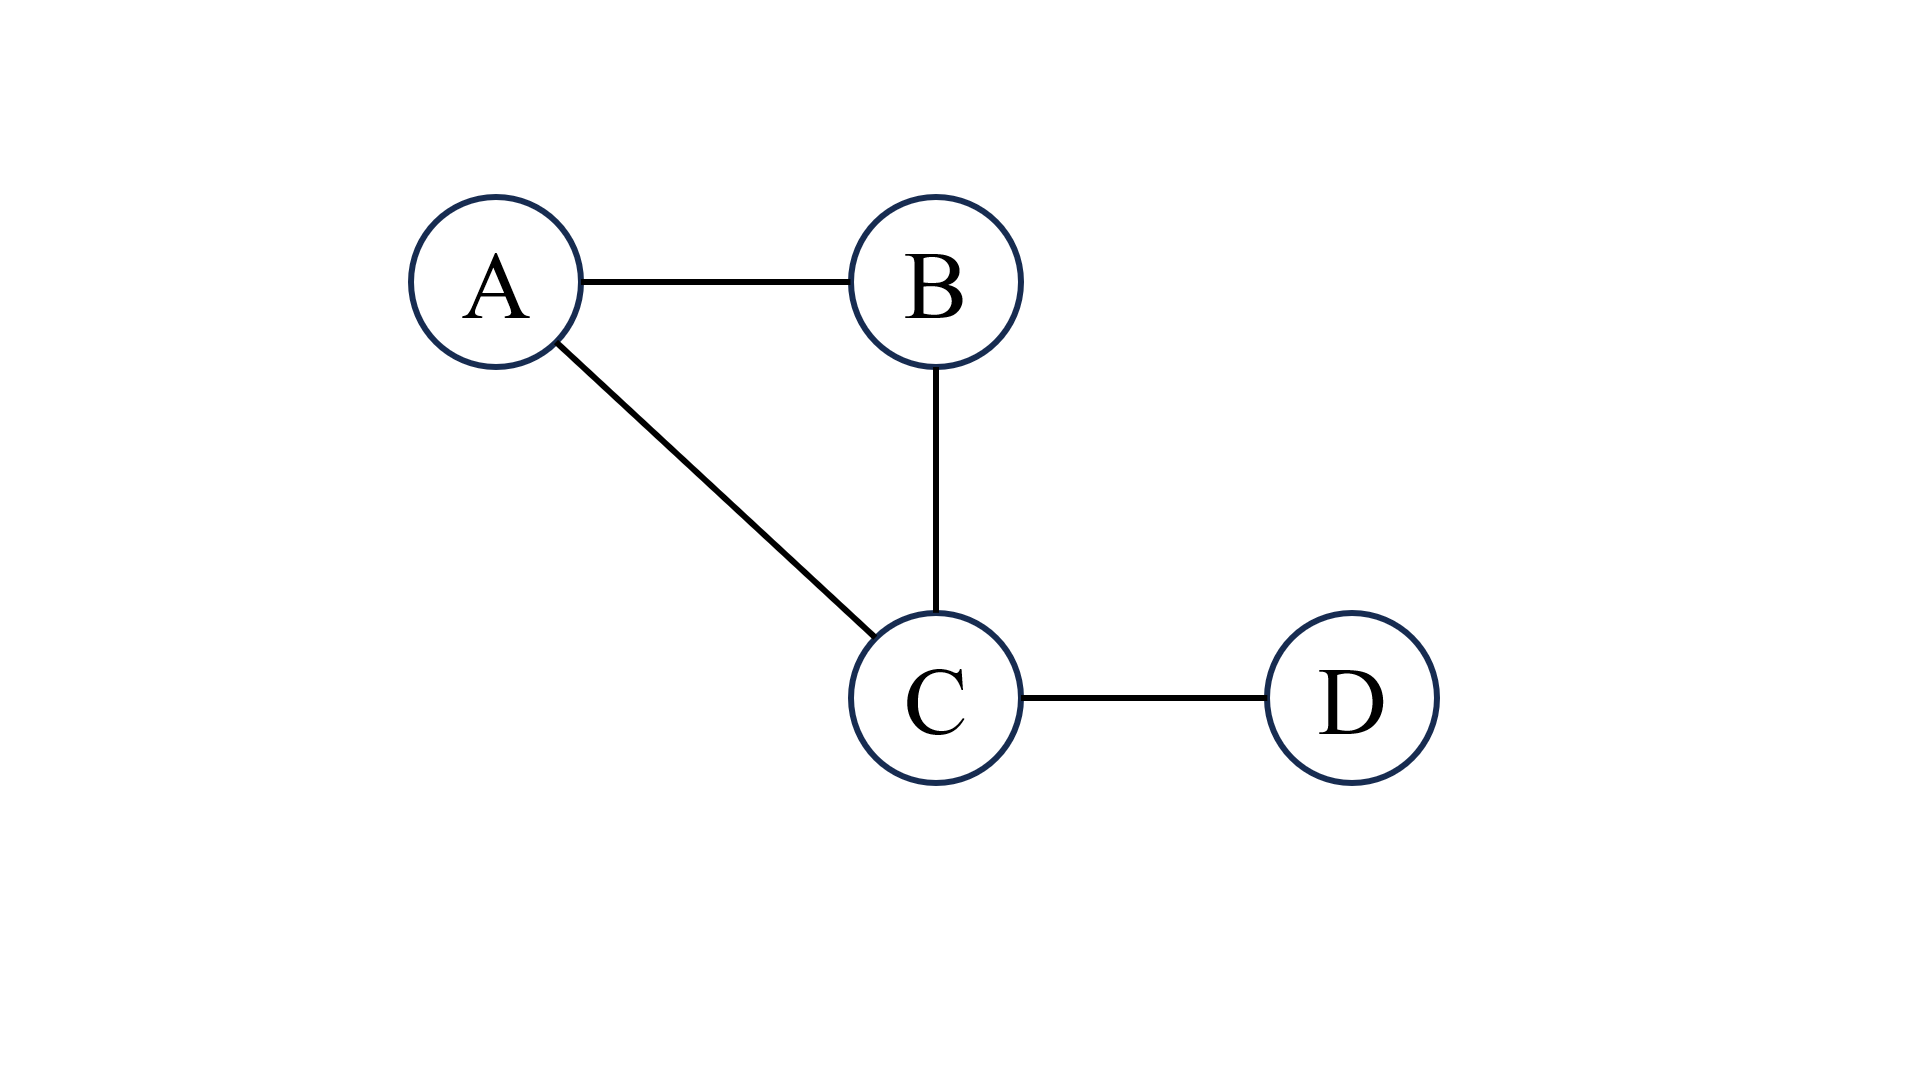
\includegraphics[width=0.48\columnwidth]{figure/chapter2/undirected_graph.png}}
  \hspace{0.02\columnwidth}
  \subfigure[Directed Graph]{%
  \label{fig:directed_graph}
  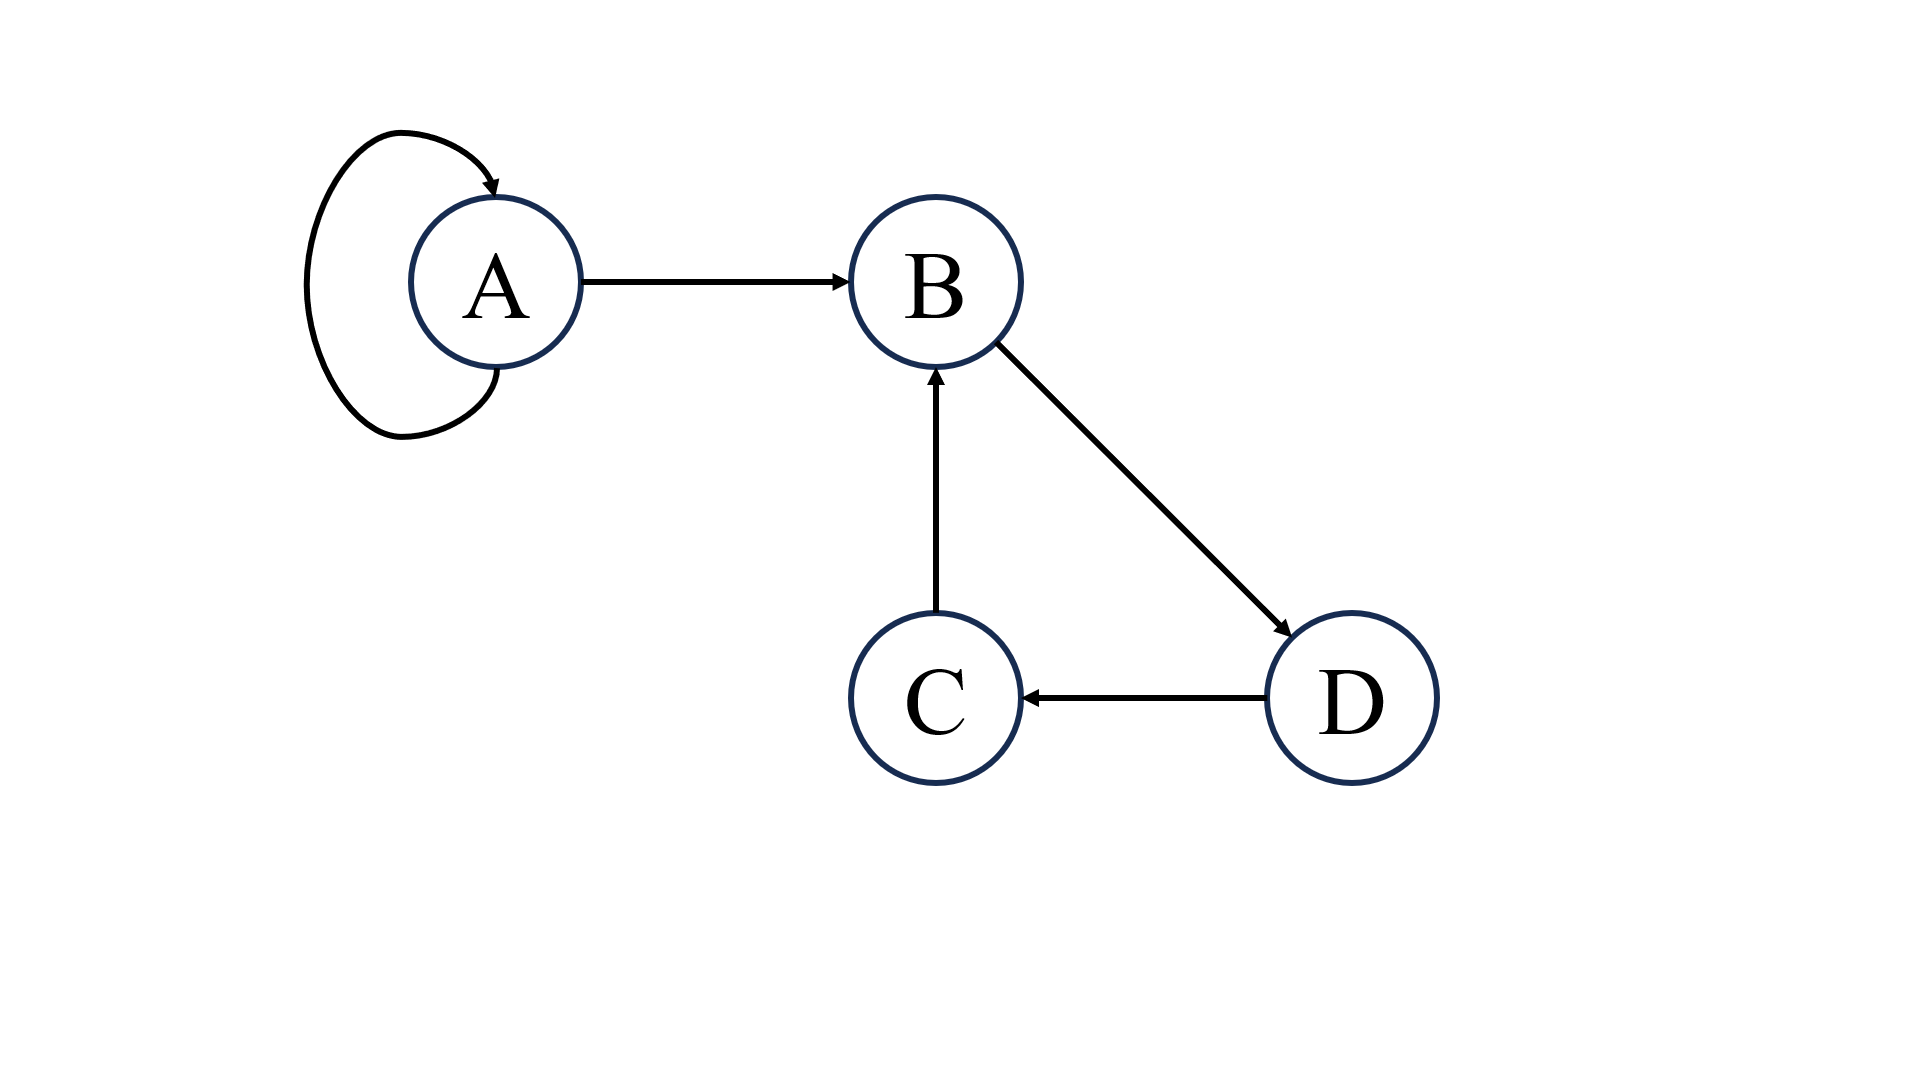
\includegraphics[width=0.48\columnwidth]{figure/chapter2/directed_graph.png}}
  \caption{Examples of simple graphs}
  \label{fig:example_simple_graphs}  % chktex 24
\end{figure}

\begin{figure}[h]
  \begin{center}
    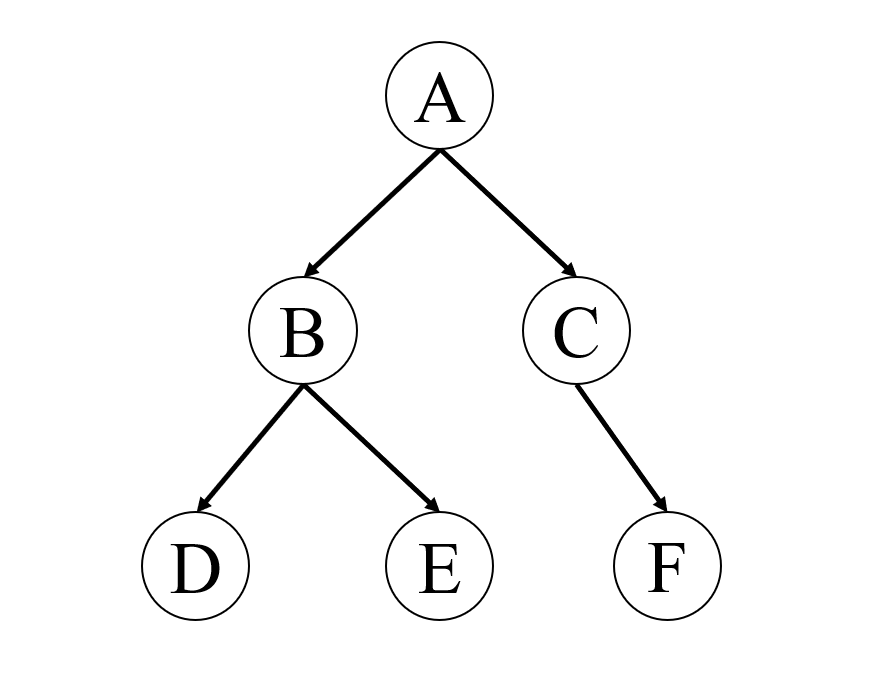
\includegraphics[width=50mm, clip]{figure/chapter2/tree_graph.png}
    \caption{Tree Graph}
    \label{fig:tree_graph} % chktex 24
  \end{center}
\end{figure}

グラフのあるノードから別のノードに到達するための経路をパスと呼び,
これを求めることをグラフ探索と呼ぶ.
グラフ探索には,深さ優先探索,幅優先探索などのさまざまなアルゴリズムが存在する.
深さ優先探索では,始点となるノードから,深さが深くなる方向を優先して探索を行う.
これに対して,幅優先探索では,始点となるノードから,深さが浅いノードを優先して探索を行う手法である.

\subsection{歩容パターングラフの定義}
本研究においては,6脚ロボットの歩容パターンをグラフを用いて表現する.
グラフはロボットの状態をノードとし,ロボットの状態間の遷移,つまりロボットの動作をエッジとして作成する.
グラフは有向の根付き木とし,現在のロボットの状態を根ノード,
その姿勢から1動作で到達できる姿勢を子ノードとして根ノードに接続する.
また,このようにして作られたグラフを歩容パターングラフと定義する.
\figref{fig:image_of_gait_pattern_graph}に歩容パターングラフのイメージを示した.

本手法では,まず歩容パターングラフを作成する.
そして,根ノードから最適な動作を行う葉ノードまでのパスをグラフ探索によって求め,
そのパスに含まれる深さ1のノードを次の動作としてロボットに実行させる.
これを繰り返すことで,ロボットの歩容パターンを生成しているのである.

グラフ探索による歩容パターン生成においては,網羅的にロボットの状態を調べ上げるため,
実時間内の計算を行うにはグラフの規模を小さくすることが求められる.
しかし,歩容パターングラフはロボットの状態や動作を対象とするため無数の組み合わせが存在し,
そのすべてを網羅的に調べ上げることは困難である.
そのため,状態や動作を離散化することで歩容パターン生成をグラフへ落とし込む必要がある.
以下に各要素の離散化方法について述べる.
\\  % 1行開ける

\begin{figure}[h]
  \begin{center}
    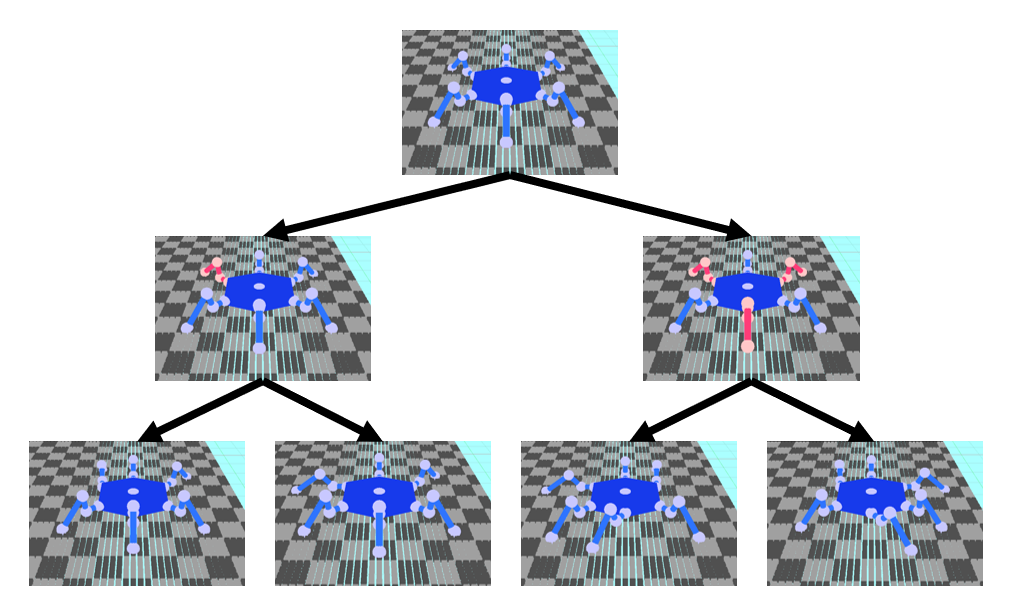
\includegraphics[width=100mm, clip]{figure/chapter2/gait_pattern_graph.png}
    \caption{Image of Gait Pattern Graph}
    \label{fig:image_of_gait_pattern_graph} % chktex 24
  \end{center}
\end{figure}

\subsubsection{グラフの階層構造}
前述のとおり,ロボットの脚位置は脚の可動範囲内であれば,無数の位置を取ることができる.
そのため本手法では,基準となる脚位置を決め,その基準からの相対位置を用いて脚位置を離散化している.
Prabirらが提案した手法では2次元平面での移動を前提としていたが\cite{Prabir_Graph_search},
これを三浦が3次元空間へ拡張した\cite{Miura_Graph_search}.

\figref{fig:discretization}に支持脚の脚位置の離散化の様子を示した.
\figref{fig:discretization}のように脚位置の基準座標を4とし,
脚位置4と同じ高さにあるかつ,進行方向に対して基準位置よりも前方にある脚位置を6,後方にある脚位置を2とする.
また,脚位置6よりも高い位置にある脚位置を7,低い位置にある脚位置を5とし,
脚位置2よりも高い位置にある脚位置を3,低い位置にある脚位置を1とする.
このようにして,脚位置を7つに離散化している.
遊脚している脚の脚位置は,支持脚の脚位置1$\sim$7に対応させ,脚位置1'$\sim$7'とする.% $\sim$ で波線を引く

これにより,脚位置1$\sim$7から脚位置1'$\sim$7'への遷移によって,脚の上下運動を表現することができる.
また,脚位置1'$\sim$7'内での遷移によって,遊脚の水平方向の移動を表現することができる.
以上より,脚の上下運動と脚の水平方向の移動をグラフで表現することができることを示した.

\begin{figure}[h]
  \begin{center}
    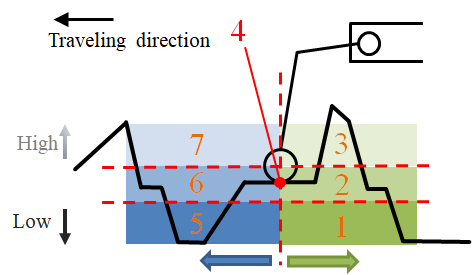
\includegraphics[width=75mm, clip]{figure/chapter2/discretization_of_leg_pos.png}
    \caption{Discretization of Leg Posistion}
    \label{fig:discretization} % chktex 24
  \end{center}
\end{figure}

このような脚位置の離散化を行うことで,脚位置の組み合わせを有限個に抑えることができるが,
脚位置の組み合わせは未だ,$7^6 = 117649 \approx 10^5$通り存在し,
遊脚である時を含めるとさらに組み合わせが増えてしまうことがわかる.
プログラムの実行環境によって左右されるが,
プログラミング言語のC++で作成した処理では約1秒間に$10^8$回程度の計算が可能であるとされており\cite{Program_Challenge_Book},
この組み合わせをすべて歩容パターングラフに追加した場合,実時間内の処理を行うにはグラフの規模が大きくなりすぎる.
そこで,大木らは脚位置の組み合わせを階層構造化することで,
遊脚時の脚位置1'$\sim$7'を省略し,探索するノード数を減らすことに成功した\cite{Oki_Graph_search}.

階層構造とこれを利用した探索の方法を説明するために,遊脚の組み合わせと脚位置の組み合わせについて定義を行う.
遊脚の組み合わせは,ロボットの各脚について,その脚が遊脚であるか支持脚であるかを表すノードの要素である.
6脚ロボットの右前脚を1番目の脚として,時計回りに2番目の脚から6番目の脚とする.
この時,i番目の脚が支持脚であることを$v_i = 1$,遊脚である時を$v_i = 0$とすると,
遊脚の組み合わせ$V$は\eqref{eq:leg_com}のように表すことができる.

\begin{equation}\label{eq:leg_com}
  V = \{v_1, v_2, v_3, v_4, v_5, v_6\}
\end{equation}

\noindent 遊脚の組み合わせは$2^6 = 64$通り存在するが,
6脚,5脚,4脚が遊脚である組み合わせや,
隣り合う3脚が遊脚である組み合わせは
実際には取りえない組み合わせであるため,
探索するべき組み合わせは$2^6 - {}_6 \mathrm{C}_6 - {}_6 \mathrm{C}_5 - {}_6 \mathrm{C}_4 - 6 = 36$通りとなる.

また,脚位置の組み合わせとは離散化した脚位置において,各脚がどの位置にあるかを表すノードの要素である.
i番目の脚が脚位置jにあることを$k_i = j$とすると,
脚位置の組み合わせ$K$は\eqref{eq:leg_pos}のように表すことができる.

\begin{equation}\label{eq:leg_pos}
  K = \{k_1, k_2, k_3, k_4, k_5, k_6\}
\end{equation}

\noindent\eqref{eq:leg_com},\eqref{eq:leg_pos}より
ロボットの脚の状態は遊脚の組み合わせ$V$と脚位置の組み合わせ$K$を用いて表すことができるようになった.
i番目の脚の状態を$l_i = v_i \cdot k_i$とすると,$L$は\eqref{eq:leg_state}のように表すことができる.

\begin{equation}\label{eq:leg_state}
  L_{ij} = \{v_1 \cdot k_1, v_2 \cdot k_2, v_3 \cdot k_3, v_4 \cdot k_4, v_5 \cdot k_5, v_6 \cdot k_6\}
\end{equation}

\noindent\eqref{eq:leg_state}より,脚位置の組み合わせが$K = \{1,1,1,1,1,1\}$で
遊脚の組み合わせが$V = \{0,1,0,1,0,1\}$である時の脚の状態を$L_{ij} = \{0,1,0,1,0,1\}$と表すことができる.
同様に,脚位置の組み合わせが$K = \{3,1,3,1,3,1\}$で遊脚の組み合わせが$V = \{0,1,0,1,0,1\}$である時の脚状態は
$L_{ij} = \{0,1,0,1,0,1\}$と表すことができる.
このことから,ある脚位置の組み合わせから,別の脚位置の組み合わせへの遷移は,
脚の状態$L$が等しいときのみ可能であることがわかる.

以上の定義より,階層構造と階層を用いたグラフの探索方法について説明することができる.
階層とは脚位置の組み合わせ$K$が等しく,かつ,遊脚の組み合わせ$V$が異なるノードの集合と定義され,
遊脚の組み合わせが36通り存在することから,同じ階層内のノードは36個存在する.
脚の上下運動を実現したい場合は,遊脚の組み合わせ$V$が異なるノードを探索する必要があるため,
図\ref{fig:hierarchy2}のように階層内のノード36個のみを探索すればよい.

また,脚の水平運動を実現したい場合は,脚位置の組み合わせ$K$が異なるノードを探索する必要があるため,
図\ref{fig:hierarchy}のように脚の状態$L$が等しくなるノードのみを探索すればよい.
脚の状態$L$が等しくなるノードは,最大で3脚が遊脚しているときの$7^3 = 343$個であるため,
十分に実時間内の計算が可能である.

\begin{figure}[htbp]
  \begin{center}
    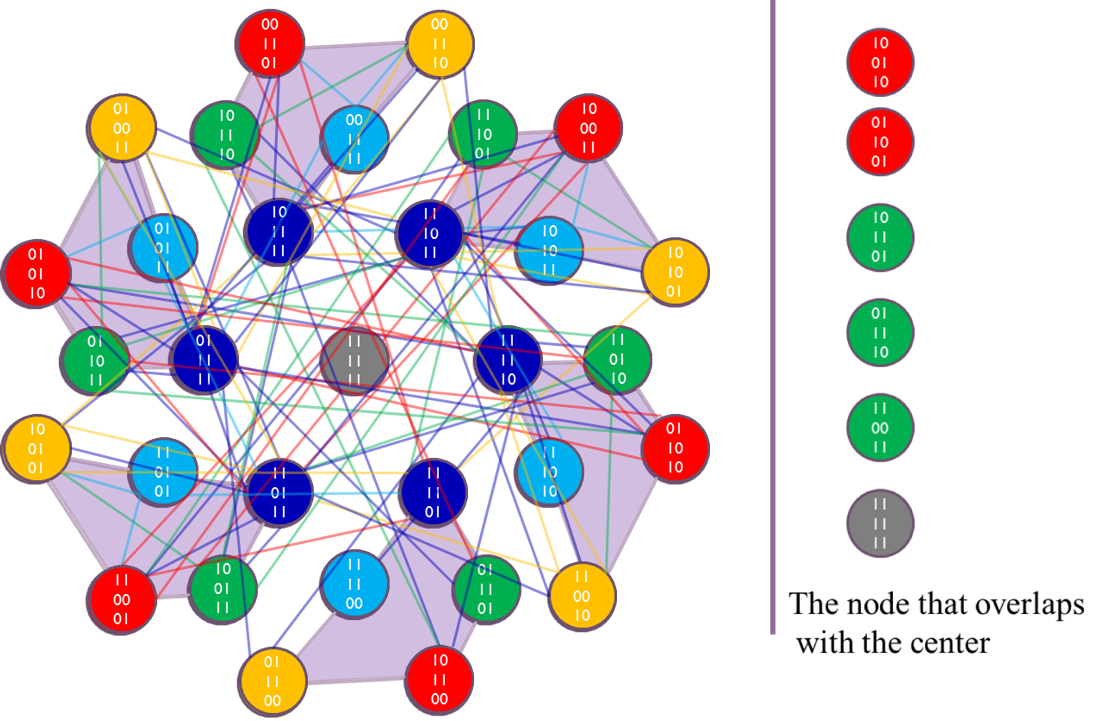
\includegraphics[width=75mm, clip]{figure/chapter2/hierarchy2.png}
    \caption{Search in the Same Hierarchy}
    \label{fig:hierarchy2} % chktex 24
  \end{center}
\end{figure}

\begin{figure}[htbp]
  \begin{center}
    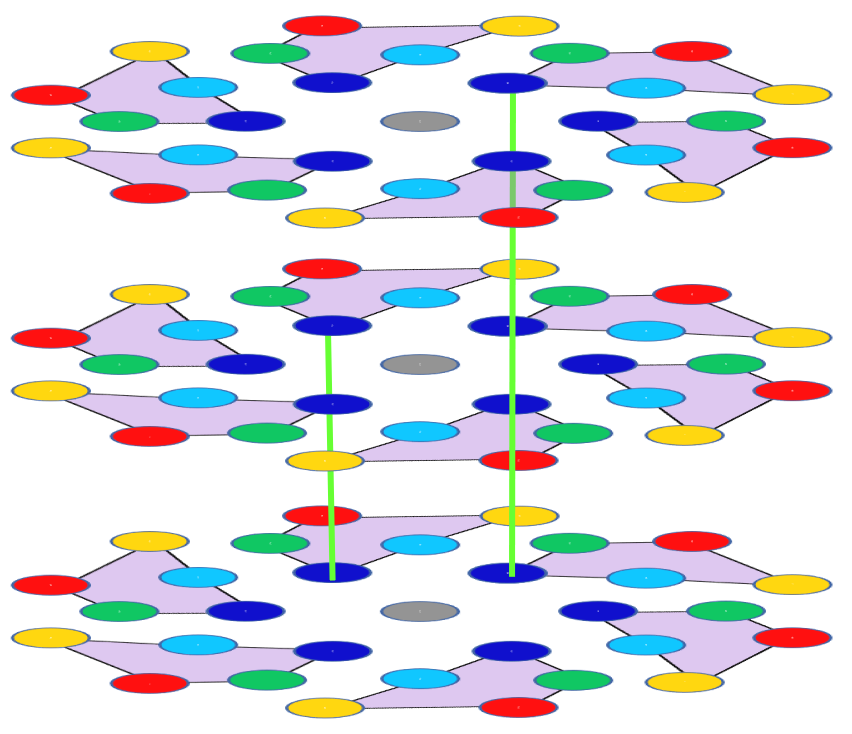
\includegraphics[width=75mm, clip]{figure/chapter2/hierarchy.png}
    \caption{Search in the Difficult Hierarchy}
    \label{fig:hierarchy} % chktex 24
  \end{center}
\end{figure}

\subsubsection{脚軌道生成の分離}
次に歩容パターングラフのエッジについて述べる.
歩容パターングラフにおいて,エッジはロボットの動作を表す.
ロボットの動作は脚の接地・遊脚運動と,重心の移動からなるため,これらの動作に対応するエッジを作成する.
具体的には,脚の上下移動のエッジ,脚の水平移動のエッジ,重心の上下移動のエッジ,
重心の水平移動のエッジ,そして,重心の回転のエッジを用いてロボットの動作を表現する.

これらのエッジには,移動前と移動後のノードを補完するための状態を持っておらず,
単純に移動前と移動後のノードを結ぶのみである.
これはつまり,歩容パターングラフを生成するプログラムと,脚軌道を生成するプログラムが分離されていることを意味する.
脚軌道を考える場合,ロボットの関節の可動範囲を考慮する必要があり,逆運動学解を用いる脚の関節角度の計算が求められる.
しかし,逆運動学の計算には計算負荷の大きい逆三角関数の計算が必要となり,各エッジについて網羅的に計算を行うことを考えると,
実時間内の計算が困難になってしまう.
そのため本手法では,歩容パターングラフを生成するプログラムを分離し,
歩容パターングラフの生成時には脚の可動範囲は近似的な値を用いて計算することで,
実時間内の計算を可能にしている.

近似された脚の可動範囲の求め方について述べる.
近似された脚の可動範囲は脚の付け根を中心とする環状の扇形として表現する.
簡単のため,以降は扇形の外径を最大半径,内径を最小半径と呼ぶことにする.
まず,脚先を届くことができる範囲を求めるために,
最大半径を以下の手順で求める.
\begin{enumerate}
  \item 脚の付け根と脚先が同じ高さになるように脚先を上げる.
  \item 図\ref{fig:leg_range_a}のように水平方向に脚先を$1 [mm]$ずつ伸ばす.
  \item 脚先を伸ばすことができなくなった場合,\\
        図\ref{fig:leg_range_b}のように脚先と脚の付け根の高さ方向の距離の差をインデックスとして,\\
        脚先と第1関節の水平方向の距離を最大半径として記録する.
  \item 脚先を$1 [mm]$下げて(2)(3)の処理を繰り返す.脚先を下げることができなくなった場合,処理を終了する.
\end{enumerate}
次に最小半径をロボットの脚長などのパラメータから決定する.
先行研究では実験で用いたロボットにあわせ,$120 [mm]$とした.
そして,扇形の中心角を隣の脚と干渉しないように決定する.
こうして求められる近似された脚の可動範囲のイメージを\figref{fig:approximated_range_of_motion}に示す.
\figref{fig:approximated_range_of_motion}では右中央の脚の近似された脚の可動範囲のみを示しており,
赤い領域で示される図形が近似された脚の可動範囲である.

このように近似を行ったことで,以下に示す手順で脚先が脚の可動範囲内にあるか判定することができる.
\begin{enumerate}
  \item 脚の付け根から脚先までの水平方向のベクトルを求め,ベクトルの傾きが扇形の中心角の範囲内にあるか判定する.
  \item 脚の付け根から脚先までの水平方向の距離を求める.
  \item 最小半径よりも大きく,最大半径よりも小さいか判定する.
  \item 以上の条件を満たす場合,脚先は脚の可動範囲内にあると判定する.
\end{enumerate}
(2)(3)の手順は四則演算のみで計算が可能であり,
(1)の手順もベクトルの内積を用いて計算が可能であるため同様に四則演算のみで計算が可能である.
そのため,脚先が脚の可動範囲内にあるかの判定を高速に行うことができる.
本手法では脚軌道生成だけでなく,脚の接地判定にもこの近似的な脚の可動範囲を用いている.


\begin{figure}[htbp]
  \subfigure[Horizontal Movement of the Leg Tips]{%
  \label{fig:leg_range_a}
  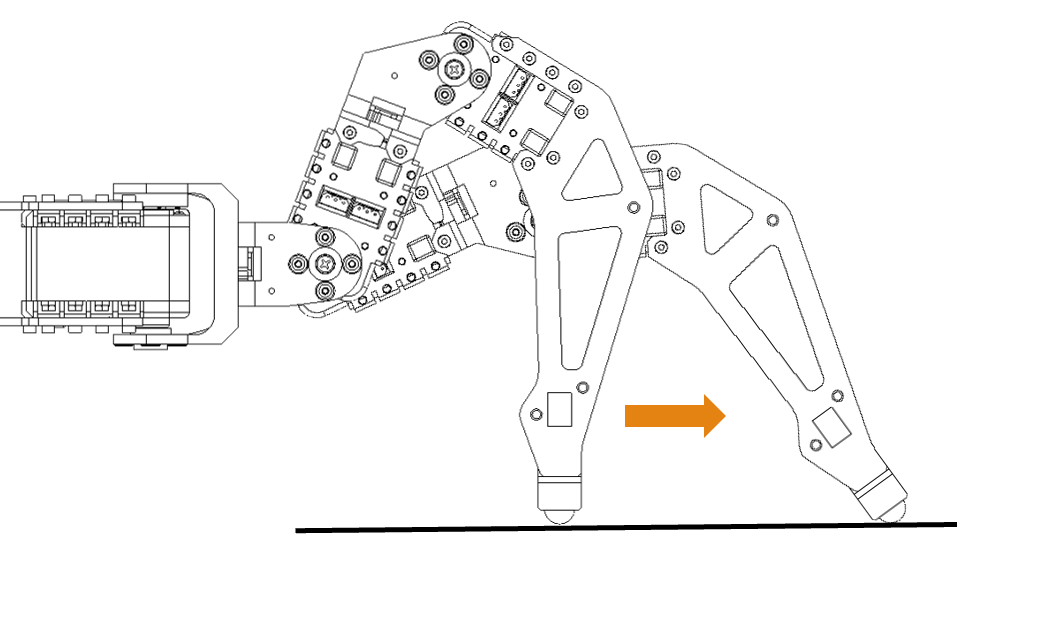
\includegraphics[width=0.48\columnwidth]{figure/chapter2/leg_range.png}}
  \hspace{0.04\columnwidth}
  \subfigure[Determination of the Maximum Radius]{%
  \label{fig:leg_range_b}
  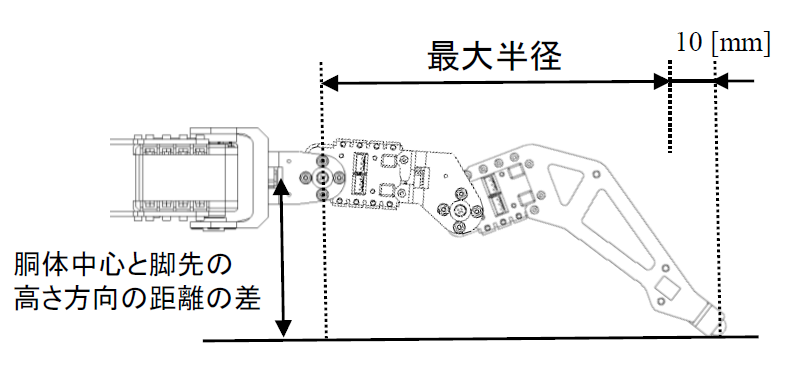
\includegraphics[width=0.48\columnwidth]{figure/chapter2/max_leg_range.png}}
  \caption{Caluculation of the Maximum Radius}
  \label{fig:leg_range}  % chktex 24
\end{figure}

\begin{figure}[htbp]
  \subfigure[Side View]{%
  \label{fig:side_view}
  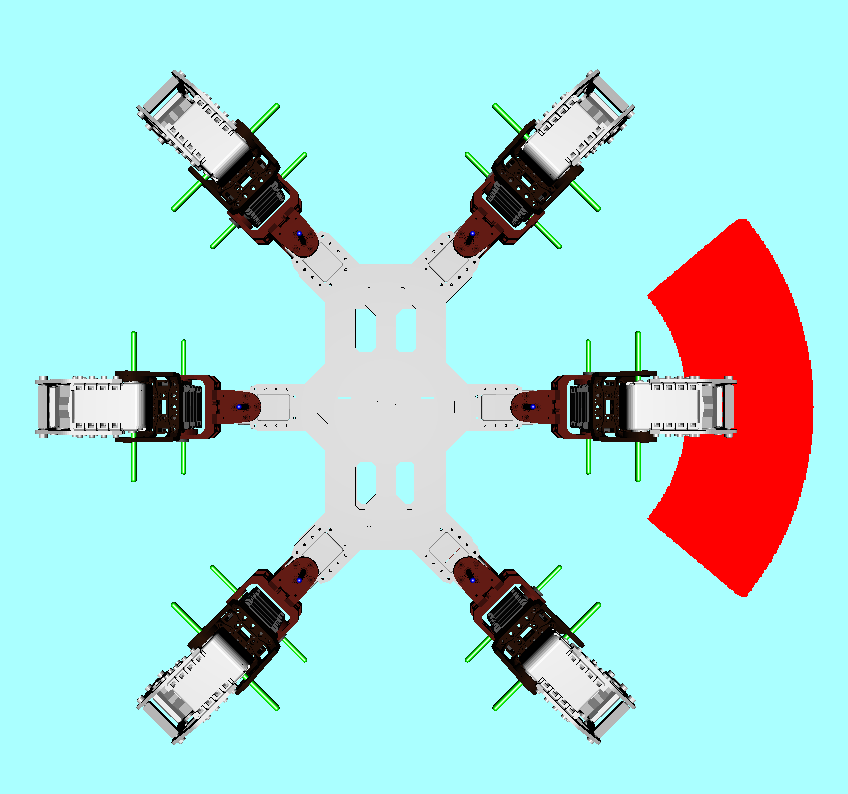
\includegraphics[width=0.48\columnwidth]{figure/chapter2/approximated_range_motion_top.png}}
  \hspace{0.04\columnwidth}
  \subfigure[Top View]{%
  \label{fig:top_view}
  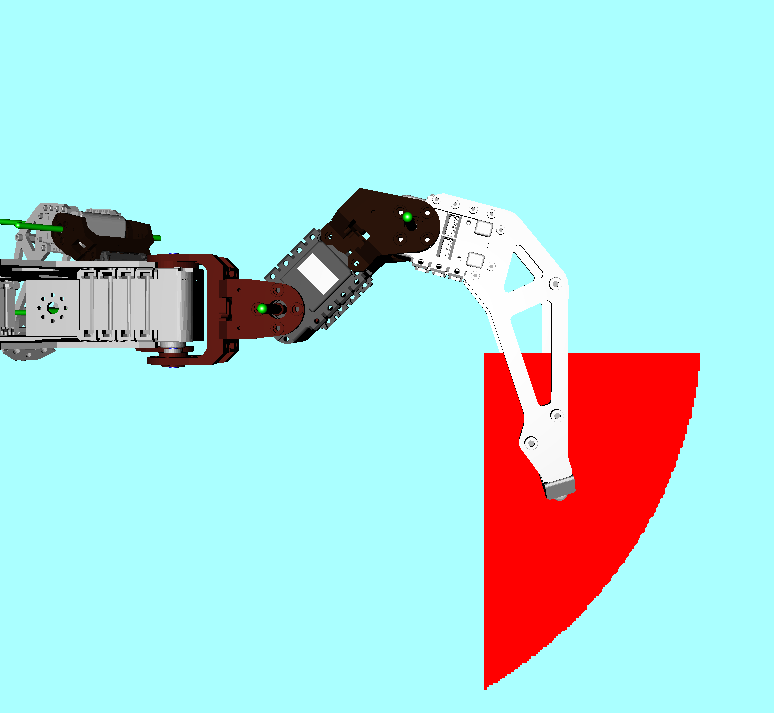
\includegraphics[width=0.48\columnwidth]{figure/chapter2/approximated_range_motion_back.png}}
  \caption{Approximated Range of Motion}
  \label{fig:approximated_range_of_motion}  % chktex 24
\end{figure}

\subsection{脚軌道生成の失敗}
先行研究ではグラフの階層構造化および脚軌道生成の分離によって,実時間内の計算が可能になった.
しかし,実際に実機を用いて歩行実験を行ったところ,低頻度ではあるが脚軌道生成に失敗することがあった.
失敗の原因として,脚の可動範囲に近似的な値を用いていることが予想される.
近似的な脚の可動範囲の境界近くは,実際には脚の可動範囲外であるが,
近似的な値を用いているために脚の可動範囲内と判定されてしまっている領域があると考えられる.
そのため,脚軌道や脚の接地点が脚の可動範囲外になってしまい,脚軌道生成に失敗することがあると考えられる.

失敗の原因についてより具体的に議論するために,脚の可動範囲の解析を行ったため,
その方法と結果を示す.
解析の対象とするロボットは,Trossen Robotics社のPhantomX Mark I\hspace{-1.2pt}I \cite{cita:phantom_x_mark_2}  % chktex 2
(以下PhantomX)とする.
PhantomX(\figref{fig:phantomx_mk2})は6脚ロボットであり,各脚に3つのアクチュエータを持つ.
また,関節配置は脚の付け根からヨー・ピッチ・ピッチの順である.

PhantomXの脚の可動範囲を求めるために,間接角度の逆運動解を求める式を導く.
まず,\figref{fig:leg_coordinate_axis}にPhantomXの脚の座標系を示す.
第1関節を原点とし,
x軸をロボットの前方方向にとり,z軸をロボットに垂直で上向きにとる.
y軸は右手座標系となるように設定する.
また簡単のため,解析には\figref{fig:joint_and_link}のようにPhantomXのアクチュエータの回転軸を結んだ仮想的なリンクを用いる.
リンク名は第1関節からCoxa Link,Femur Link,Tibia Linkであり,関節名はCoxa Joint,Femur Joint,Tibia Jointである.
リンク長は第1関節から第3関節までそれぞれ$L_c$,$L_t$,$L_f$とし,
間接角度をそれぞれ$\theta_c$,$\theta_t$,$\theta_f$とする.
間接の座標は$P_c$,$P_t$,$P_f$とし,脚先の座標を$P_{end}$とする.
$P_{end} = \{x_{end},y_{end},z_{end}\}$の時の
このとき$P_c$,$P_f$,$P_t$,$\theta_c$,$\theta_f$,$\theta_t$を
求める式は\eqref{eq:theta_c}から\eqref{eq:theta_t}である.

\begin{align}
  P_c &= \{0,0,0\} \label{eq:theta_c} \\
  \theta_c &= \arctan \frac{y_{end}}{x_{end}}  \\
  P_f &= \{L_c \cos \theta_c, L_c \sin \theta_c, 0\}  \\
  \theta_f &= \arctan \frac{z_{end}}{\sqrt{x_{end}^2 + y_{end}^2} - L_c} + 
  \arccos \frac{L_t^2 + L_f^2 - x_{end}^2 - y_{end}^2 - z_{end}^2}{2 \cdot L_t \cdot L_f} \\
  P_t &= \{(L_c + L_t \cos \theta_f)\cos \theta_c ,
                  L_t \cos \theta_f \sin \theta_c , 
                  L_t \sin \theta_f\}  \\
  \theta_t &= \arctan \frac{z_{end} - z_t}{\sqrt{x_{end}^2 + y_{end}^2} - 
              \sqrt{x_t^2 + y_t^2}} - \theta_f \label{eq:theta_t} 
\end{align}

\newpage

% phantomx mk - 2 の図
\begin{figure}[h]
  \begin{center}
    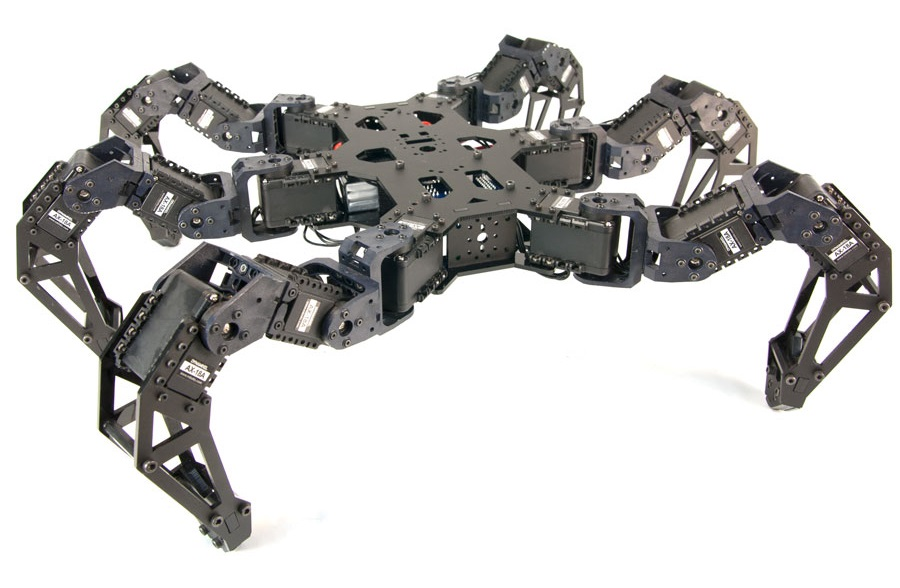
\includegraphics[width=60mm, clip]{figure/chapter2/phantomx_mk2.jpg}
    \caption{PhantomX Mark I\hspace{-1.2pt}I}
    \label{fig:phantomx_mk2} % chktex 24
  \end{center}
\end{figure}

% 脚の座標系
\begin{figure}[h]
  \begin{tabular}{cc}
    \begin{minipage}{0.5\textwidth}
      \centering
      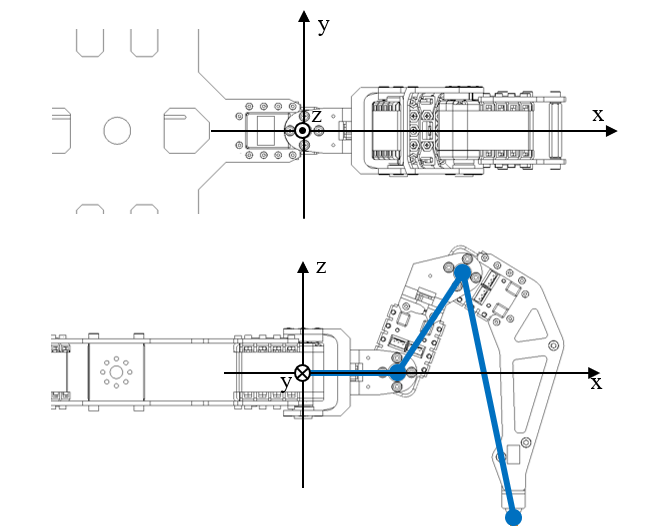
\includegraphics[width=1.0\linewidth]{figure/chapter2/coordinate_axis.png}
      \caption{Leg Coordinate Axis}
      \label{fig:leg_coordinate_axis} % chktex 24
    \end{minipage}
    \begin{minipage}{0.5\textwidth}
      \centering
      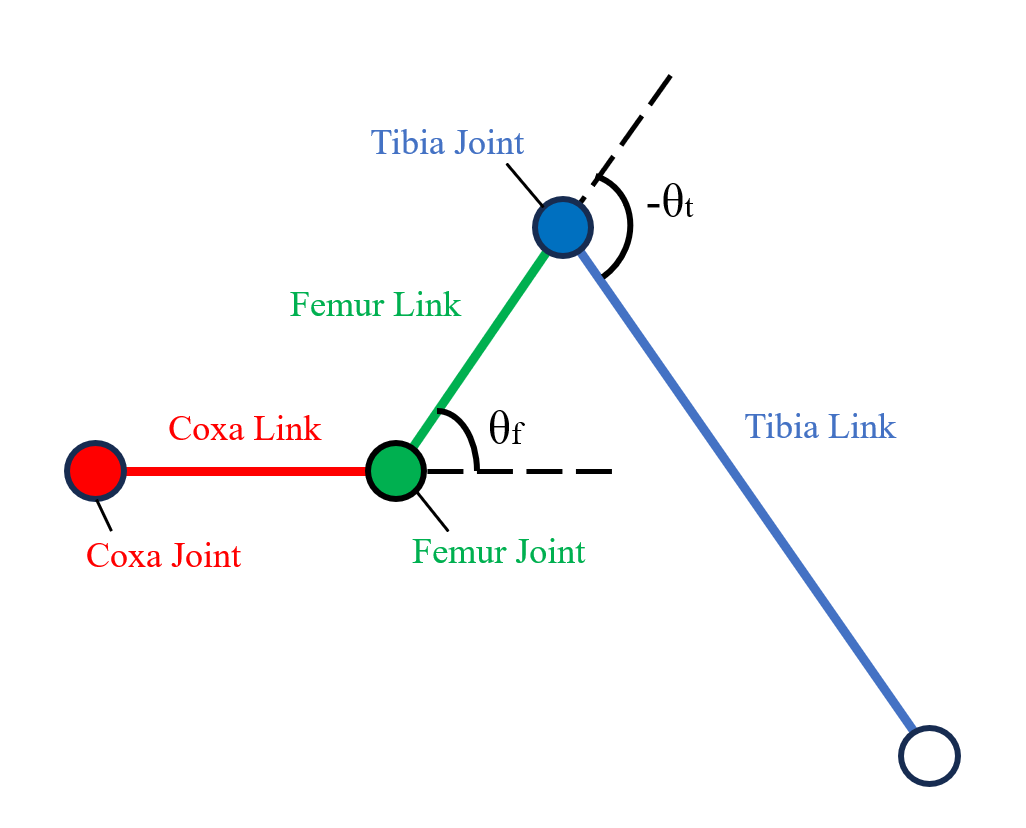
\includegraphics[width=1.0\linewidth]{figure/chapter2/link_joint.png}
      \caption{Joint and Link Name} 
      \label{fig:joint_and_link} % chktex 24
    \end{minipage}
  \end{tabular}
\end{figure}

% 脚長の表
\begin{table}[h]
	\caption{Link Length of PhantomX}
	\label{tab:link_len_phantom_x}  % chktex 24
	\begin{center}
   	\begin{tabular}{|c||c|} \hline  % chktex 44
      Link Name & $[mm]$ \\ \hline  % chktex 44
      Coxa Link & 52  \\ \hline  % chktex 44
      Femur Link & 66  \\ \hline  % chktex 44
      Tibia Link & 130  \\ \hline  % chktex 44
    \end{tabular}
  \end{center}
\end{table}

\newpage

以上の式を用いて,PhantomXの脚の可動範囲を求めたものが\figref{fig:simu_leg_range}である.
\figref{fig:simu_leg_range}では,$\theta_c = 0$とし,x-z平面における脚の可動範囲を示している.
黒色の実線で示される領域が実際の脚の可動範囲であり,緑色の実線で示される領域が近似された脚の可動範囲である.
赤色の点線で示される直線は遊脚の高さを表しており,この直線よりも高く上げることはない.

\begin{figure}[h]
  \begin{tabular}{cc}
      \begin{minipage}{0.5\textwidth}
          \centering
          
\includegraphics[width=1.0\linewidth]{figure/N_A.png}
          \caption{Approximated Range of Motion in Simulation}
          \label{fig:simu_leg_range} % chktex 24
      \end{minipage}
      \begin{minipage}{0.5\textwidth}
          \centering
          
\includegraphics[width=1.0\linewidth]{figure/N_A.png}
          \caption{Approximated Range of Motion in Experimental Equipment}
          \label{fig:act_leg_range} % chktex 24
      \end{minipage}
  \end{tabular}
\end{figure}

% 予備実験の章
\section{歩行シミュレーションによる脚軌道生成失敗時の脚先位置の特定}

\subsection{シミュレーション実験の目的}
先行研究では脚軌道生成の失敗による動作の停止が報告された上,
その原因は脚先が脚の可動範囲の外を通ることによるものであると考察されてきた.
しかし,具体的にどのような理由で脚軌道生成が失敗するのかは明らかにされていなかった.
そのため予備実験として,波東らの研究\cite{Hato_Graph_search}の実機試験と同じ条件で歩行シミュレーション実験を行う.
実験の目的は脚軌道生成の失敗の回数,接地時の脚位置,そして脚軌道を確認することで,脚軌道生成失敗の原因を特定することとする.

波東らは段差のある地形と斜面のある地形でシミュレーション,および実機による直進歩行動作の実験を行った.
また,実機試験時にはシミュレーション実験と歩行時の条件を変更していた.
本シミュレーションでは,波東らの研究のシミュレーションと実機試験それぞれの条件で歩行シミュレーションを行う.

\subsection{シミュレーションの条件}
本研究室ではロボットの動作のシミュレーションを行うためのシミュレーターソフトウェアを自作し,
シミュレーション実験を行ってきた.
本論文でも同様に,シミュレーション実験に自作のシミュレーターソフトウェアを用いた.

シミュレーターはC++で記述されており,WindowsAPIを用いてGUIを実装し,ロボットを表示している.
また,GUIの表示のプログラムをより簡単に記述するため,
ゲームプログラミングに用いられるライブラリのDxLib\cite{Dxlib_Web}を用いている.
シミュレーターは物理演算を行っておらず,トルク不足や摩擦,脚先の滑りによるずれを考慮していない.
そのため,ロボットのアクチュエータは無限のトルクを持ち,脚先は滑りなく接地するものと仮定している.
本来これらのパラメータを考慮すべきではあるが,
本研究においては歩容パターン生成によって得られた脚接地点に脚先を届かせることが可能であるか確認することが目的であるため,
これらのパラメータは考慮しないこととしている.

\subsubsection{シミュレーションの計算環境}
シミュレーションの計算環境は\tableref{tab:simulation_env}に示した.

\subsubsection{モデルとするロボット}
モデルとするロボットは\figref{fig:phantomx_mk2}のPhantomX Mark I\hspace{-1.2pt}Iとする.

\subsubsection{歩行する地形}
歩行する地形を\figref{fig:terrain}に示す.
地形は5種類あり,それぞれ平地,上り段差,下り段差,上り斜面,下り斜面である.
実機試験の条件に合わせ,段差は上り,下りともに高さが$100 [mm]$とし,
斜面は上り,下りともに角度が$15 [\deg]$とした.

\subsubsection{歩行する時の条件}

% 計算環境の表
\begin{table}[htbp]
	\caption{Simulation Environment}
	\label{tab:simulation_env}  % chktex 24
	\begin{center}
   	\begin{tabular}{|c||c|} \hline  % chktex 44
      CPU & 11thGen Intel Core (TM) i5--11400  \\ \hline  % chktex 44
      RAM & 32.0GB  \\ \hline  % chktex 44
      OS & Windows 11 Home  \\ \hline  % chktex 44
      開発環境 & Visual Studio 2022 Community  \\ \hline  % chktex 44
      使用言語 & C++20  \\ \hline  % chktex 44
    \end{tabular}
  \end{center}
\end{table}



% 地形の図
\begin{figure}[htbp]
  \begin{tabular}{cc}
    \begin{minipage}[t]{0.45\hsize}
      \begin{center}
      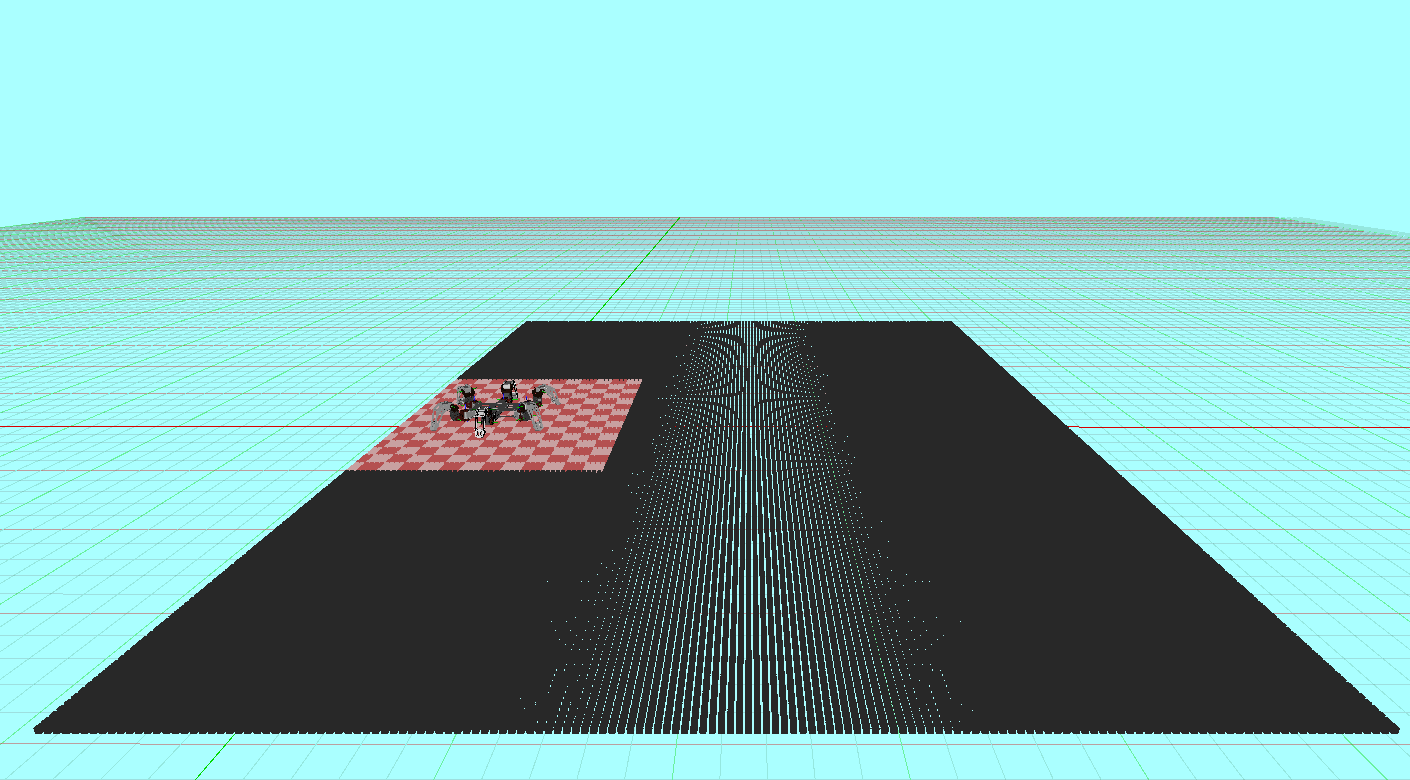
\includegraphics[width=1.0\linewidth]{figure/chapter2/map_flat.png}
      \text{(a) flat}
      \label{fig:flat_terrain} % chktex 24
      \end{center}
    \end{minipage} 
    &
    \begin{minipage}[t]{0.45\hsize}
      \begin{center}
      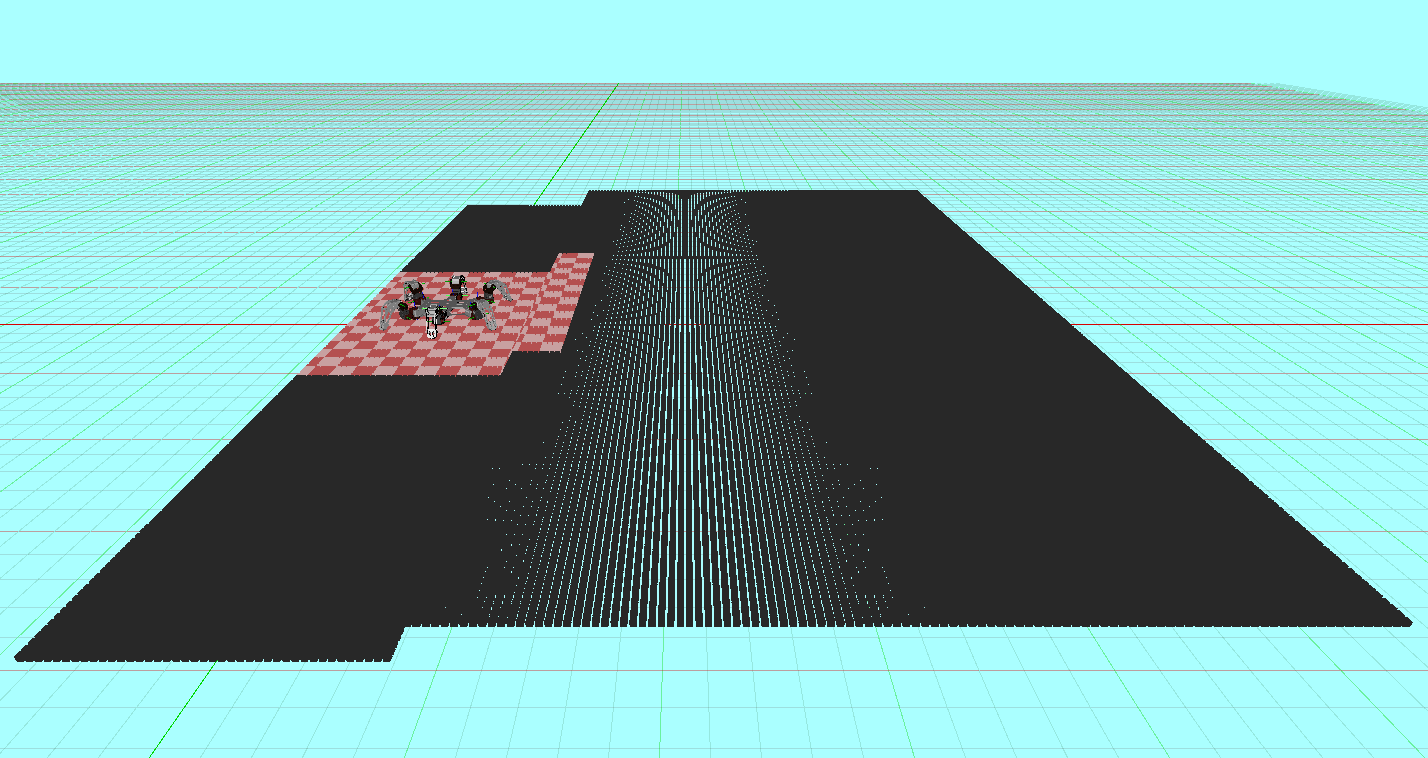
\includegraphics[width=1.0\linewidth]{figure/chapter2/map_100.png}
      \text{(b) up step}
      \label{fig:up_step_terrain} % chktex 24
      \end{center}  
    \end{minipage}
    \\
    &\\  % 空白を入れる
    \begin{minipage}[t]{0.45\hsize}
      \centering
      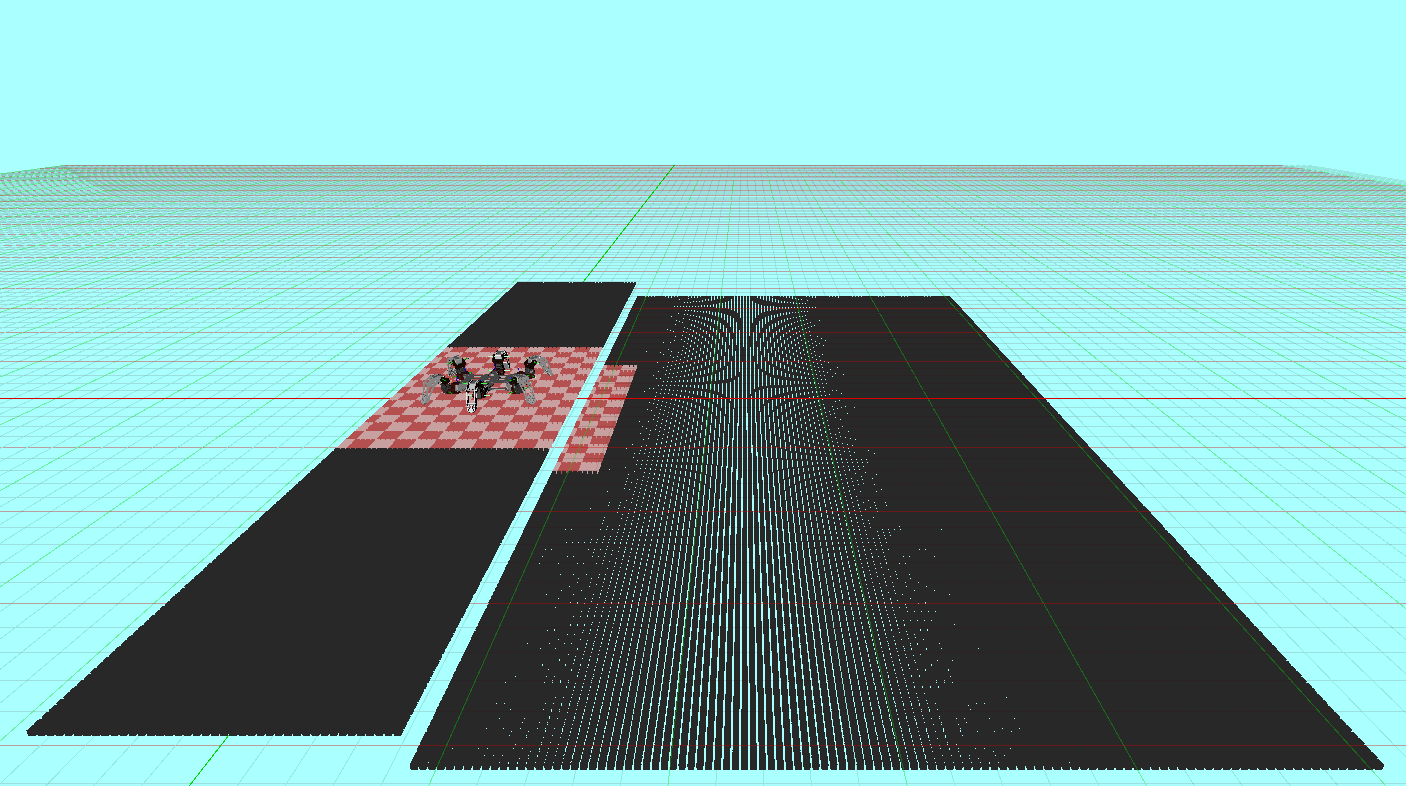
\includegraphics[width=1.0\linewidth]{figure/chapter2/map_-100.png}
      \centering
      \text{(c) down step}
      \label{fig:down_step_terrain} % chktex 24
    \end{minipage} 
    &
    \begin{minipage}[t]{0.45\hsize}
      \centering
      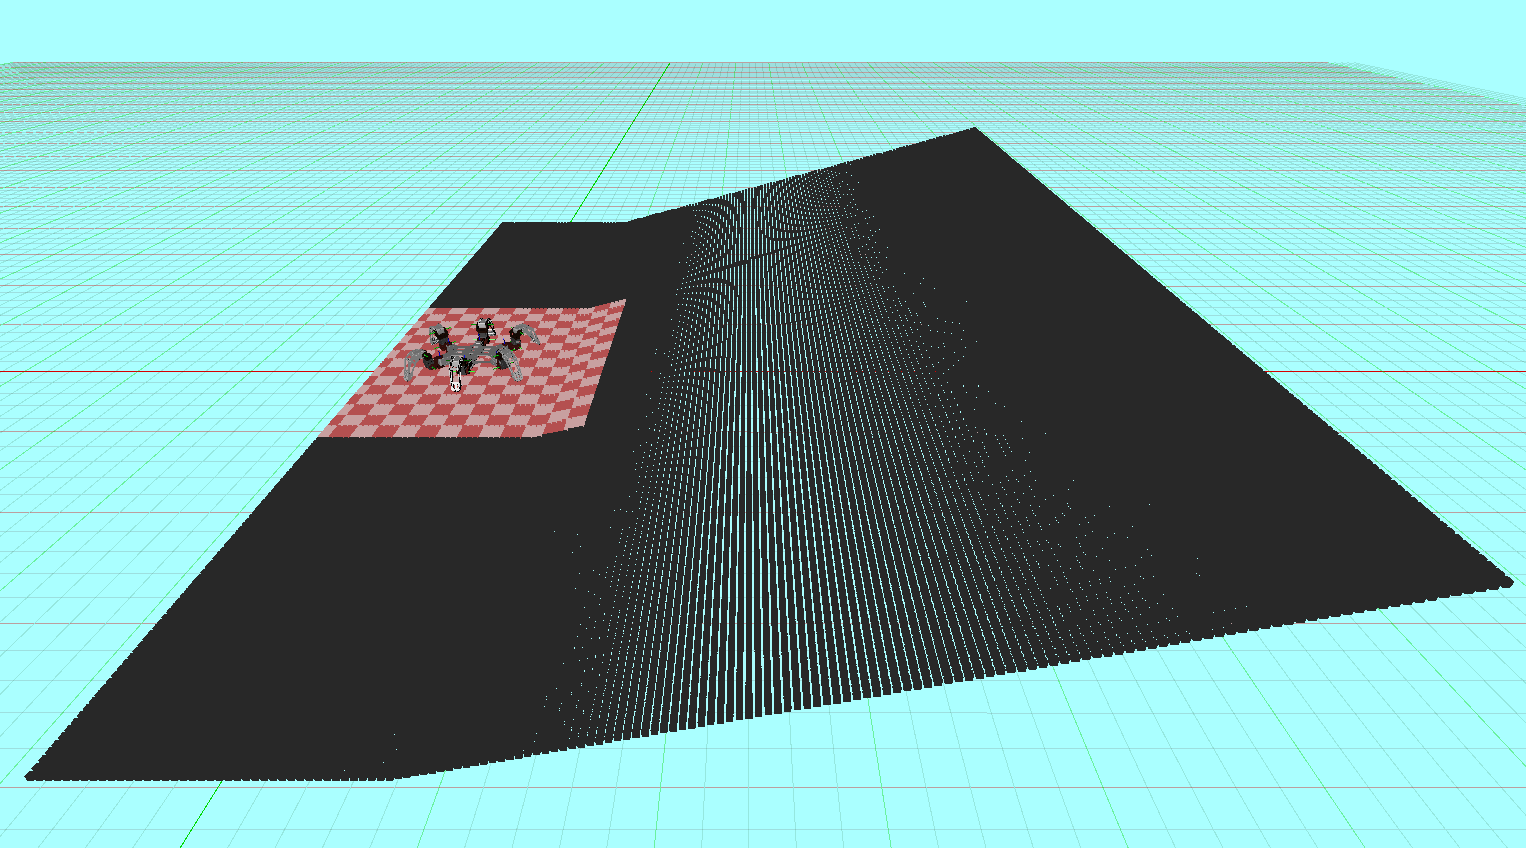
\includegraphics[width=1.0\linewidth]{figure/chapter2/map_15deg.png}
      \centering
      \text{(d) up slope}
      \label{fig:up_slope_terrain} % chktex 24
    \end{minipage}    
    \\
    &\\  % 空白を入れる
    \begin{minipage}[t]{0.45\hsize}
      \centering
      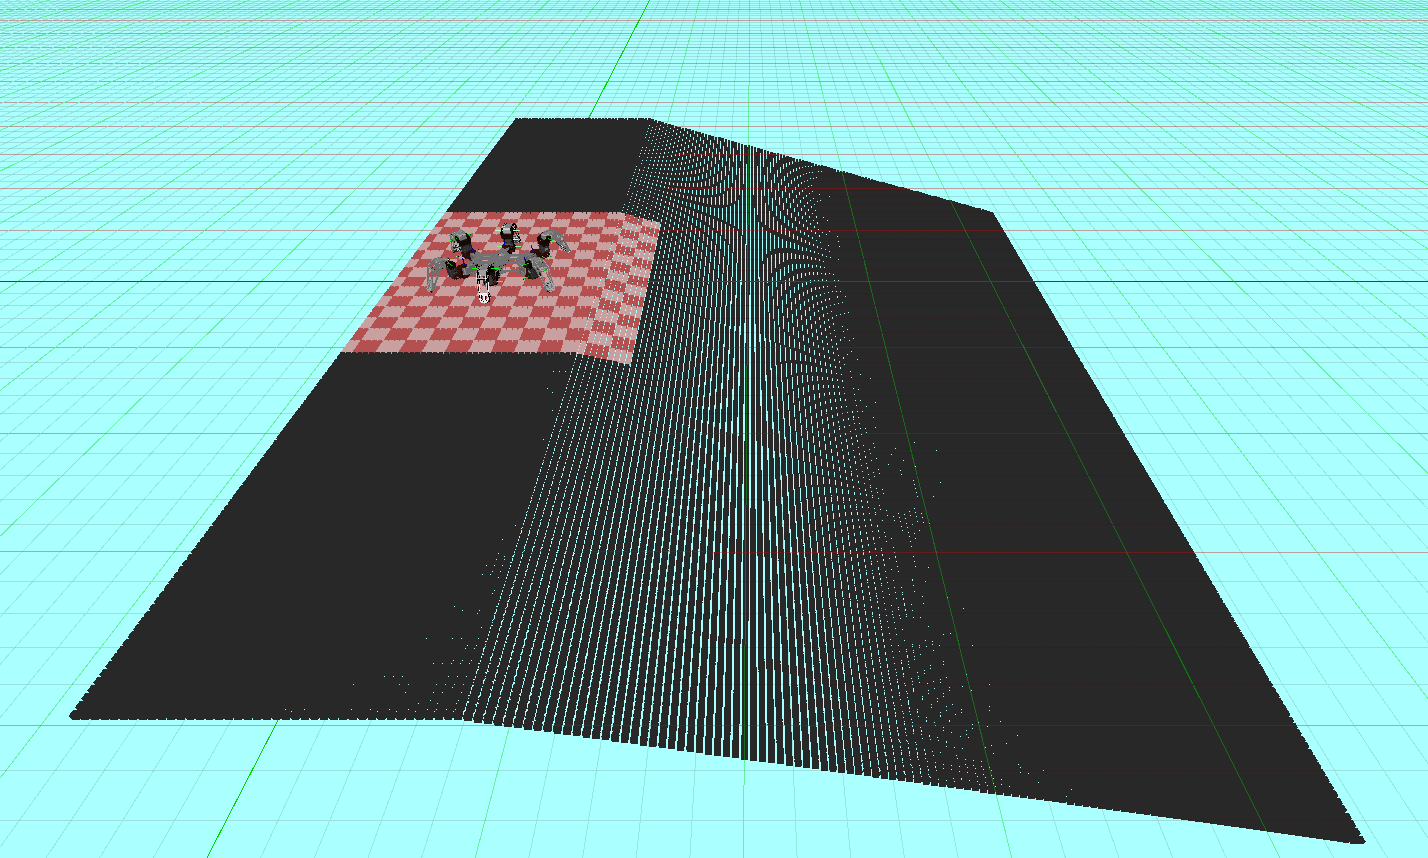
\includegraphics[width=1.0\linewidth]{figure/chapter2/map_-15deg.png}
      \centering
      \text{(e) down slope}
      \label{fig:down_slope_terrain} % chktex 24
    \end{minipage}     
    &
    \\
  \end{tabular}
  \caption{Terrain}
  \label{fig:terrain} % chktex 24
\end{figure}

\subsection{シミュレーションの結果}
まず,脚軌道生成失敗の回数を\tableref{tab:failure_count}に示す.

% 書き方 https://uec.medit.link/latex/table.html

\begin{table}[htbp]
  \caption{Failure Count of Experimental Equipment}
  \label{tab:failure_count_experimental}  % chktex 24
  \centering
  \begin{tabular}{|c|c|c|c|c|c|c|} \hline  % chktex 44
    \multirow{3}{*}{地形} & \multirow{3}{*}{グラフ探索} & \multicolumn{5}{c|}{失敗の回数} \\ \cline{3-7}  % chktex 44
     & & \multirow{2}{*}{脚接地点が} & \multicolumn{3}{c|}{脚軌道が可動範囲外を通る} & \multirow{2}{*}{総失敗} \\ \cline{4-6}  % chktex 44
     & の回数 & 可動範囲外 & 遊脚時 & 接地時 & \begin{tabular}{c}胴体平行\\移動時\end{tabular} & 回数 \\ \hline  % chktex 44
    平面     & 351 & 0 & 9 & 2 & 0 & 11 \\ \hline  % chktex 44
    上り斜面 & 645 & 0 & 10 & 1 & 0 & 11 \\ \hline  % chktex 44
    下り斜面 & 867 & 0 & 20 & 9 & 0 & 29 \\ \hline  % chktex 44
    上り段差 & 461 & 0 & 6 & 10 & 0 & 16 \\ \hline  % chktex 44
    下り段差 & 383 & 0 & 9 & 0 & 0 & 9 \\ \hline  % chktex 44
  \end{tabular}
\end{table}
 
\begin{table}[htbp]
  \caption{Failure Count of Simulation}
  \label{tab:failure_count_simulation}  % chktex 24
  \centering
  \begin{tabular}{|c|c|c|c|c|c|c|} \hline  % chktex 44
    \multirow{3}{*}{地形} & \multirow{3}{*}{グラフ探索} & \multicolumn{5}{c|}{失敗の回数} \\ \cline{3-7}  % chktex 44
     & & \multirow{2}{*}{脚接地点が} & \multicolumn{3}{c|}{脚軌道が可動範囲外を通る} & \multirow{2}{*}{総失敗} \\ \cline{4-6}  % chktex 44
     & の回数 & 可動範囲外 & 遊脚時 & 接地時 & \begin{tabular}{c}胴体平行\\移動時\end{tabular} & 回数 \\ \hline  % chktex 44
    平面     & 315 & 47 & 16 & 4 & 0 & 67 \\ \hline  % chktex 44
    上り斜面 & 460 & 63 & 11 & 22 & 1 & 97 \\ \hline  % chktex 44
    下り斜面 & 611 & 29 & 53 & 28 & 0 & 110 \\ \hline  % chktex 44
    上り段差 & 368 & 50 & 16 & 10 & 0 & 76 \\ \hline  % chktex 44
    下り段差 & 331 & 33 & 39 & 6 & 0 & 78 \\ \hline  % chktex 44
  \end{tabular}
\end{table}

\subsection{脚軌道生成に失敗する原因の考察}

% 再評価手法の提案の章
\section{歩容パターンの再評価手法}
脚軌道生成の失敗を防ぐためには近似された脚の可動範囲を小さくするか,
より正確に近似することで誤差をなくせばよい.
しかし,前者は脚の接地点として選択される領域を縮めてしまうことになるため,
グラフ探索による手法の利点である効率的な動作ができなくなってしまうことや,
本来歩行可能であった地形を歩くことができなくなってしまうことなどの問題点がある.
また,後者は細かく正確に近似するとキャッシュしておく値が増えるため,
あらかじめ計算しておいた値にアクセスする際の呼び出しにかかる時間が長くなってしまう.
これにより,計算時間が長くなってしまう問題点がある.
先行研究のプログラムでは前者の方法でこの問題に対応をしていたが,
結果的にシミュレーション時に歩行することが可能だった地形を,
実機試験時では歩行することができなくなってしまっていた.

私はグラフ探索の再評価を行うことで,脚軌道生成の失敗を防ぐことを提案する.
ここでグラフ探索の再評価とは,
グラフ探索による歩容パターン生成に成功し,脚軌道生成に失敗した場合,
グラフ探索による歩容パターン生成をやり直して,脚軌道生成に失敗しない新しい歩容パターンを生成することを指す.
歩容パターン生成をやり直す際,脚軌道生成に失敗しないよう,脚の近似された可動範囲を狭め,
可動範囲外に接地することがないようにする.
こうして歩容パターングラフを再生成し,グラフ探索を再度行うことで,
脚軌道生成に失敗しないノードを取得することが可能となる.

再評価手法は前述した2つの解決法と比べ,それらのもつ問題点を克服している.
以下にそれぞれの解決策と比較した再評価手法の利点を示す.

\begin{description}
  \item[可動範囲を小さくすることによる,本来接地可能だった地点を選択できなくなってしまう問題]\mbox{}\\
    脚の可動域をある程度広く確保することが可能になり,
    可動範囲の境界に近い点を接地点として選択できるようになる.
    加えて,脚軌道生成に失敗する場合,狭められた可動域に切り替えて失敗を防ぐことができる.
  \item[より正確に近似された脚の可動範囲を確保する場合に,値を呼び出す際にかかる時間が増えてしまう問題]\mbox{}\\
    再評価手法では歩容パターン生成をやり直す都合上,
    単純計算で探索にかかる時間が倍になってしまう.
    よってより正確に近似する方が実行時間的に優れると思える.
    しかし,歩容パターングラフの生成時には $10^5 ~ 10^6$ 程度の数のノードを生成するため,
    グラフ探索内の処理の時間の増加は,最終的な計算時間を大幅に増加させてしまう可能性がある.
    つまり再評価手法では計算時間の増加を約 2 倍程度で済ませることができるといえる.
\end{description}
 % 第2章
    %% 歩容パターンの再評価手法の実装.tex
%% LaTeX-2e 専用

\chapter{歩容パターンの再評価手法の実装}\label{chapter:歩容パターンの再評価手法の実装}
第\ref{chapter:歩容パターンの再評価手法の実装}章では,
第\ref{chapter:歩容パターンの再評価手法の提案}章で述べた歩容パターンの再評価手法の実装方法について述べる.

\section{グラフ探索による自由歩容パターン生成手法の実装}
再評価手法の実装方法の説明の前に,3次元空間におけるグラフ探索による自由歩容パターン生成手法の実装方法について述べる.
波東らが用いた自由歩容パターン生成手法による直進動作と同様の手法によって歩容パターンを生成しているが,
より早い処理の実現やプログラムの可読性・拡張性の向上のため,その実装方法を1部変更している.
加えて,新たに3次元空間における旋回動作の実装と先行研究の手法の統合を行ったため,変更点を含め,改めて実装方法を説明する.

プログラムの実装はC++20を用いて行っており,命名規則はGoogle~C++~Style~Guide\cite{cita:google_cpp_style_guide}にしたがっている.
開発にはVisual~Studio~2022を用いており,プログラムのビルドにはVisual~Studio~2022のMSVCコンパイラを用いている.

また,この章におけるクラスや構造体の図はUML(Unified~Modeling~Language)を用いて表現されており,
上からクラス・構造体の名前,メンバ変数,メンバ関数を表している.
メンバ変数は,アクセス修飾子,変数名,型の順に記述されており,
メンバ関数は,アクセス修飾子,関数名,引数,戻り値の順に記述されている.
アクセス修飾子は記号を用いて表し,+はpublic,protectedは\#,
privateは$-$である.
クラス間の関係は,継承関係は空白の三角形,集約関係は空白の菱形で表している.
集約関係とは,クラスのメンバ変数として他のクラスを持つことを表している.

\subsection{プログラム全体の流れ}
グラフ探索による自由歩容パターン生成手法では,
歩容パターングラフの作成,歩容パターングラフの探索の2つの処理を行う.
歩容パターングラフを作成する処理はGraphTreeCreatorクラスで実装されており,
歩容パターングラフの探索を行う処理はGraphSearcherクラスで実装されている.

これらの処理の流れを\figref{fig:graph_search_sequence}に示す.
まず,GraphTreeCreatorクラスに現在のロボットの状態を表すノードを渡す.
GraphTreeCreatorクラスは渡されたノードを根ノードとする歩容パターングラフを作成する.
次に,GraphSearcherクラスに作成された歩容パターングラフを渡す.
このとき値をコピーして渡すのではなく,
ポインタを渡すことでメモリの使用量を削減するとともに,
グラフ探索の処理時間を短縮している.
GraphSearcherクラスは渡された歩容パターングラフを探索し,
最適な次の動作を見つけて返す.
以上の流れでグラフ探索による自由歩容パターン生成手法を実装している.

\figref{fig:graph_search_class_diagram}にグラフ探索による自由歩容パターン生成手法を実装したクラスのクラス図を示す.
GaitPatternGeneratorBasicクラスは,自由歩容パターン生成手法を実装したクラスである.
GaitPatternGeneratorBasicクラスは,IGaitPatternGeneratorインターフェイスを継承しており,
メンバ関数としてGetNextNodeByGraphSearch関数を持っている.
GetNextNodeByGraphSearch関数は,現在のロボットの状態を表すノードを引数,
地形の情報,目標位置・目標姿勢を引数に取り,グラフ探索によって最適な歩容パターンを返す.
IGaitPatternGeneratorインターフェイスを介することで,
後述する再評価手法の実装や,グラフ探索による自由歩容パターン生成手法の切り替えを容易にしている.
メンバ変数にGraphTreeCreatorクラスのポインタと,
IGraphSearcherインターフェイスを継承したクラスのポインタをもっており,
GaitPatternGeneratorBasicクラスのコンストラクタでそれぞれ初期化される.

GraphTreeCreatorクラスは,歩容パターングラフの作成を行うクラスである.
メンバ変数にINodeCreatorインターフェイスのポインタの配列を持っており,
行う動作によって異なるINodeCreatorクラスを用いてグラフを作成する.
IGraphSearcherインターフェイスは,グラフ探索を行う処理を表すインターフェイスである.
歩容パターングラフの作成,歩容パターングラフの探索はそれぞれ
行う動作によって異なる方法で処理を行うためインターフェイスを作成している.

\begin{figure}[htbp]
  \begin{center}
    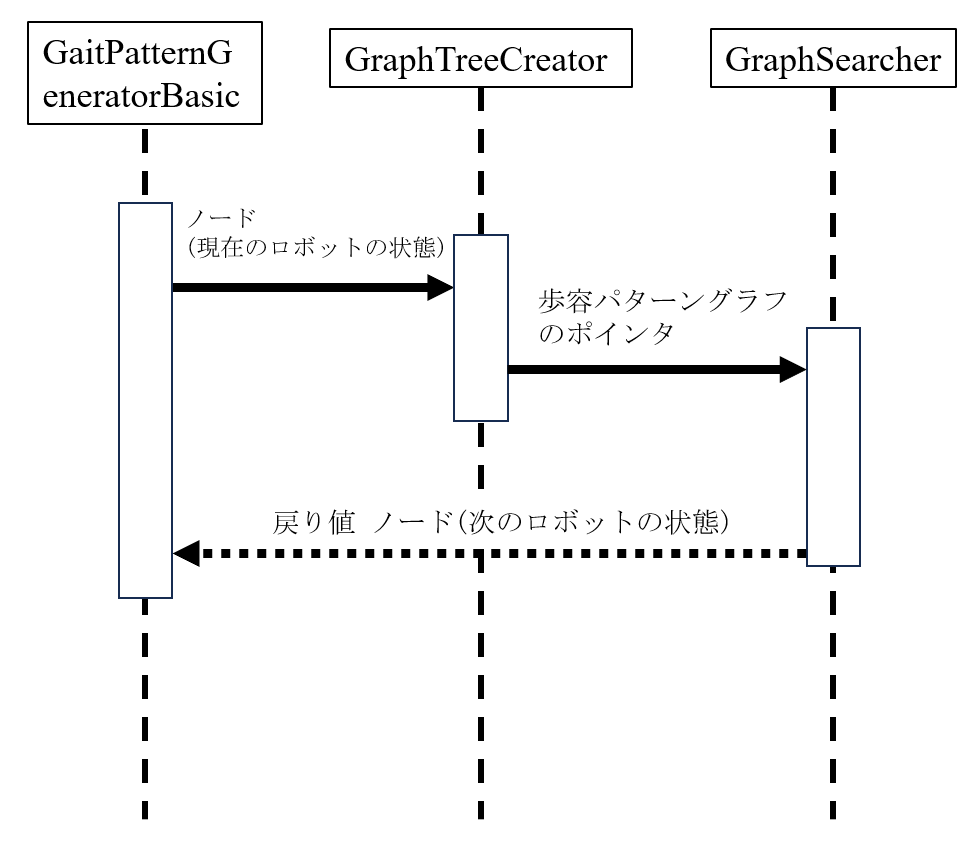
\includegraphics[width=65mm, clip]{figure/chapter3/sequence_main.png}
    \caption{Graph Search Sequence}
    \label{fig:graph_search_sequence} % chktex 24
  \end{center}
\end{figure}

\begin{figure}[htbp]
  \centering
  \begin{tikzpicture}  % [show background grid]
    \begin{interface}[text width=70mm]{IGaitPatternGenerator}{-12, -7.5}
      \attribute{}
      \operation{+ GetNextNodeByGraphSearch() }
    \end{interface}

    \begin{class}[text width=70mm]{GaitPatternGeneratorBasic}{-12, 0}
      \implement {IGaitPatternGenerator}
      \attribute{- graph\_searcher\_ptr\_ : std::unique\_ptr\textless~IGraphSearcher~\textgreater}
      \attribute{- graph\_tree\_creator\_ptr\_ : std::unique\_ptr\textless~GraphTreeCreator~\textgreater}
      \attribute{- graph\_tree\_ : GaitPatternGraphTree}
      \operation{+ GetNextNodeByGraphSearch(\newline
      \qquad current\_node : RobotStateNode, \newline 
      \qquad map : MapState, \newline 
      \qquad operation : RobotOperation, \newline
      \qquad output\_node\_ptr : RobotStateNode*) : \newline
      \qquad void }
    \end{class}

    \begin{interface}[text width=60mm]{IGraphSearcher}{-4, -4}
      \attribute{}
      \operation{+ SearchGraphTree() }
    \end{interface}

    \begin{class}[text width=60mm]{GraphTreeCreator}{-4, 0}
      \attribute{- node\_creator\_map\_ : std::map\textless~HexapodMove, std::unique\_ptr\textless~INodeCreator~\textgreater~\textgreater}
      \operation{+ Init() }
      \operation{+ CreateGraphTree() }
    \end{class}

    \begin{class}[text width=60mm]{GaitPatternGraphTree}{-4, -7}
      \attribute{- nodes\_ : std::vector\textless~RobotStateNode~\textgreater}
      \attribute{- graph\_size\_ : int}
    \end{class}

    \aggregation{GaitPatternGeneratorBasic}{}{}{IGraphSearcher}
    \aggregation{GaitPatternGeneratorBasic}{}{}{GraphTreeCreator}
    \aggregation{GaitPatternGeneratorBasic}{}{}{GaitPatternGraphTree}

  \end{tikzpicture}
  \caption{Graph Search Class Diagram}
  \label{fig:graph_search_class_diagram}  % chktex 24
\end{figure}

\newpage

\subsection{ノードを表現する構造体}
次に,歩容パターングラフを作成する処理を記述するために,ノードについて説明する.
歩容パターングラフのノードは\figref{fig:robot_state_node}のような,
ロボットの状態を表す構造体RobotStateNodeで表現した.
歩容パターングラフではRobotStateNodeを配列とすることで作成するため,
RobotStateNode構造体はサイズを小さくし,メモリの使用量を少なくすることが求められる.

RobotStateNodeのメンバ変数leg\_stateは,ロボットの脚の状態を表すビット列である.
C++の標準ライブラリのstd::bitsetを用いて実装されており,28ビットの長さを持つ.
ビット列の各ビットは,\figref{fig:leg_state_bit}のように定義されている.
下位24bitは各脚の離散化された脚位置と遊脚状態を表し,上位4bitは後述するロボットの重心位置を表す.
このようにすることで複数のパラメータを1つの変数のみで表現することができ,
メモリの使用量を削減することができる.

leg\_posとleg\_reference\_posは,ロボットの脚の位置を表すVector3構造体の配列である.
Vector3構造体は,3次元ベクトルを表す構造体であり,\figref{fig:vector3}のように定義されている.
leg\_posはロボットの脚の現在の位置を表し,leg\_reference\_posは離散化された脚位置の脚位置4の位置を表す.
座標系は脚の付け根を原点とするローカル座標系であり,単位はmmである.

center\_of\_mass\_global\_coordとpostureは,
グローバル座標におけるロボットの重心位置と姿勢を表すVector3構造体とQuaternion構造体である.
Quaternion構造体は,クォータニオンを表す構造体であり,\figref{fig:quaternion}のように定義されている.

next\_moveは,次に行う動作を表すHexapodMove列挙型である.
先行研究ではint型で表現していたが,可読性の向上のために列挙型を用いている.
parent\_indexは,親ノードのインデックスを表すint型である.
先行研究では親ノードへのポインタを用いていたが,
自身の実行環境ではポインタのサイズは8byteであるため,
4byteのint型を用いることでメモリの使用量を削減している.
depthは,ノードの深さを表すint型である.
RobotStateNodeは以上のように定義されており,188byteのサイズである.

このノードを用いて歩容パターングラフを作成する際,
根ノードはparent\_indexを$-1$,depthを$0$に設定する.
その後,根ノードのnext\_moveを基に子ノードを作成し,
parent\_indexを根ノードのインデックス,depthを$1$に設定する.
こうして作成した子ノードのnext\_moveを基に,
さらに子ノードを作成することで歩容パターングラフを作成できる.
歩容パターングラフはRobotStateNode構造体の配列で表現できるが,
処理を簡単にするためGaitPatternGraphTreeクラスでラッパーしている.

RobotStateNode構造体とVector3構造体,Quaternion構造体は
それぞれメンバ変数を操作するためのメンバ関数を持っているが,
グラフ探索の処理とは直接的な関係がないため,ここでは説明を省略する.
\\ 

\begin{figure}[htbp]
  \centering
  \begin{tikzpicture}
    \begin{class}[text width=8cm]{RobotStateNode}{0, 0}
      \attribute{+ leg\_state : std::bitset\textless 28\textgreater}
      \attribute{+ leg\_pos : std::array\textless Vector3, 6\textgreater}
      \attribute{+ leg\_reference\_pos : std::array\textless Vector3, 6\textgreater}
      \attribute{+ center\_of\_mass\_global\_coord : Vector3}
      \attribute{+ posture : Quaternion}
      \attribute{+ next\_move : HexapodMove}
      \attribute{+ parent\_index : int}
      \attribute{+ depth : int} 
      \operation{}
    \end{class}
  \end{tikzpicture}
  \caption{RobotStateNode Struct}
  \label{fig:robot_state_node}  % chktex 24
\end{figure}

\begin{figure}[htbp]
  \begin{tabular}{cc}
    \begin{minipage}[t]{0.45\hsize}
      \centering
      \begin{tikzpicture}
        \begin{class}[text width=6cm]{Vector3}{0, 0}
        \attribute{+ x : float}
        \attribute{+ y : float}
        \attribute{+ z : float}
        \operation{}
        \end{class}
      \end{tikzpicture}
      \caption{Vector3 Struct}
      \label{fig:vector3}  % chktex 24
    \end{minipage}
    &
    \begin{minipage}[t]{0.45\hsize}
      \centering
      \begin{tikzpicture}
        \begin{class}[text width=6cm]{Quaternion}{0, 0}
          \attribute{+ w : float}
          \attribute{+ v : Vector3}
          \operation{}
        \end{class}
      \end{tikzpicture}
      \caption{Quaternion Struct}
      \label{fig:quaternion}  % chktex 24
    \end{minipage}       
  \end{tabular}
\end{figure}

\begin{figure}[htbp]
  \begin{center}
    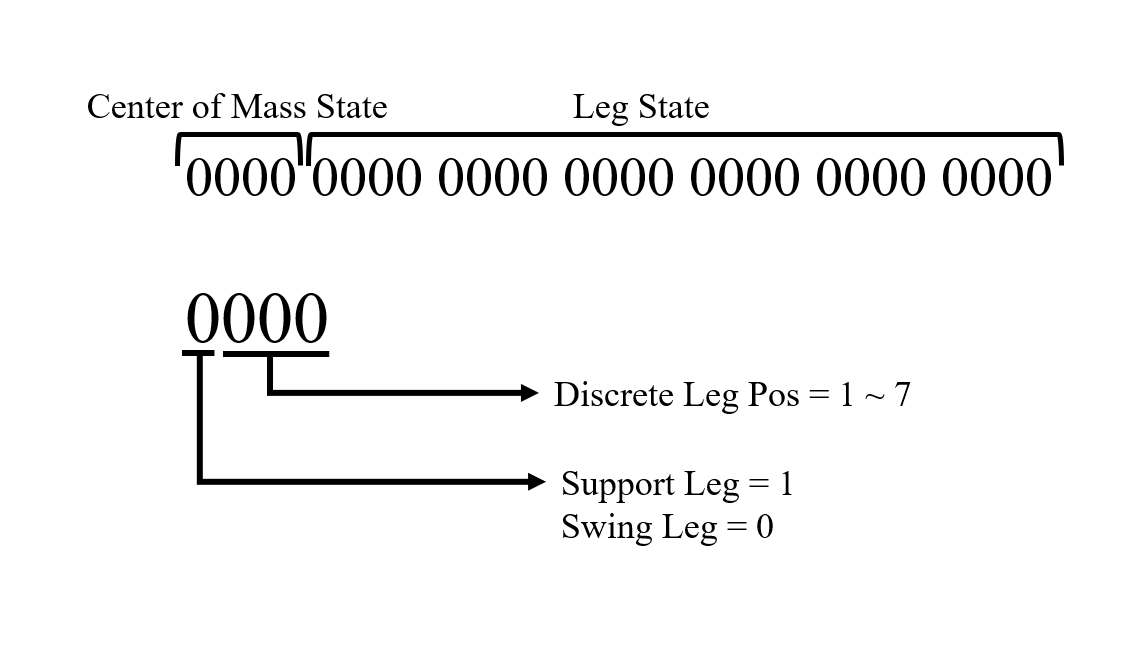
\includegraphics[width=80mm, clip]{figure/chapter3/leg_state.png}
    \caption{Leg State Bit}
    \label{fig:leg_state_bit} % chktex 24
  \end{center}
\end{figure}

\subsection{目標位置・目標姿勢を表現する構造体}
ロボットの目標位置・目標姿勢を表現するRobotOperation構造体を\figref{fig:robot_operation}に示す.
メンバ変数のoperation\_type\_はロボットの動作を表す列挙型,RobotOperationType型の変数である.
この変数の値によってロボットの行うべき動作が決定される.
これはつまり,グラフ探索において高く評価されるノードが変更されるということである.
operation\_type\_以外の変数は具体的にどのような動作を行うかを表し,
operation\_type\_の値によって使用する変数が決定される.

operation\_type\_の値と使用する変数の対応を\tableref{tab:robot_operation_type_enum}に示す.
直進動作を行う場合,指定することができるのはkStraightMoveVectorとkStraightMovePositionの2つである.
kStraightMoveVectorは,ロボットの進行方向を単位ベクトルのstraight\_move\_vector\_で指定する.
kStraightMovePositionは,ロボットの目標位置をstraight\_move\_position\_で指定する.

その場旋回動作を行う場合,指定することができるのはkSpotTurnLastPostureとkSpotTurnRotAxisの2つである.
kSpotTurnLastPostureは,ロボットの旋回前の姿勢をspot\_turn\_last\_posture\_で指定する.
kSpotTurnRotAxisは,ロボットの旋回軸をspot\_turn\_rot\_axis\_で指定し,その軸周りに右ねじの方向に旋回する.
\\

% RobotOperation 構造体の説明
\begin{figure}[h]
  \centering
  \begin{tikzpicture}
    \begin{class}[text width=7cm]{RobotOperation}{0, 0}
      \attribute{+ operation\_type\_ : RobotOperationType}
      \attribute{+ straight\_move\_vector\_ : Vector3}
      \attribute{+ straight\_move\_position\_ : Vector3}
      \attribute{+ spot\_turn\_last\_posture\_ : Quaternion}
      \attribute{+ spot\_turn\_rot\_axis\_ : Vector3}
      \operation{}
    \end{class}
  \end{tikzpicture} 
  \caption{RobotOperation Struct}
  \label{fig:robot_operation}  % chktex 24
\end{figure}

% RobotOperationTypeの列挙型をテーブルにする
\begin{table}[h]
  \caption{RobotOperationType Enum}
  \label{tab:robot_operation_type_enum}  % chktex 24
  \begin{center}
    \begin{tabular}{|c|c|} \hline  % chktex 44
      \backslashbox{動作}{要素} & RobotOperationType \\ \hline  % chktex 44
      \multirow{2}{*}{直進} & kStraightMoveVector \\ \cline{2-2}  % chktex 44
      & kStraightMovePosition \\ \hline  % chktex 44
      \multirow{2}{*}{その場旋回} & kSpotTurnLastPosture \\ \cline{2-2}  % chktex 44
      & kSpotTurnRotAxis \\ \hline  % chktex 44
    \end{tabular}
  \end{center}
\end{table}

\newpage

\subsection{地形を表現する構造体}
地形を表現するMapState構造体を\figref{fig:map_class_diagram}に示す.
グラフ探索においては連続的な地形を離散化する必要があるため,
地形を離散化するための点群を表す配列map\_point\_をメンバ変数に持っている.
map\_point\_はVector3構造体の配列であり,脚の接地可能点を表す.
map\_point\_は地形を上から見た時,格子状に配置されており,
隣の脚接地可能点との間隔は一定で$20 [mm]$である.
この間隔はロボットの脚先の面積を考慮して決定した.

MapState構造体を用いることで地形を離散化することができるが,
依然として脚接地可能点の数は多い.
そのため,ロボットを中心に地形を分割し,
各分割領域における脚接地可能点を表すDividedMapState構造体を作成した.
\figref{fig:map_view}において,赤い点で表される脚接地可能点がDividedMapState構造体で表現されている.
DividedMapState構造体は,グローバル座標におけるロボットの重心位置を表すglobal\_robot\_com\_を中心に
地形を分割した際の,各分割領域における脚接地可能点を表すdivided\_map\_point\_をメンバ変数に持っている.
また,各分割領域の最上点の高さを表すdivided\_map\_top\_z\_をメンバ変数に持っている.
脚の接地判定を行う際は,DividedMapState構造体の中から脚先に近い領域群を選択し,
その領域群における脚接地可能点を用いて接地判定を行うことで,
計算する脚接地可能点の数を減らしている.
\\

% MapState 構造体の説明
\begin{figure}[h]
  \centering
  \begin{tikzpicture}
    \begin{class}[text width=7cm]{MapState}{0, 2}
      \attribute{+ map\_point\_ : std::vector~\textless~Vector3~\textgreater}
      \operation{}
    \end{class}

    \begin{class}[text width=7cm]{DividedMapState}{0, 0}
      \attribute{+ global\_robot\_com\_ : Vector3}
      \attribute{+ divided\_map\_point\_ : std::vector~\textless~std::vector~\textless~Vector3~\textgreater~\textgreater}
      \attribute{+ divided\_map\_top\_z\_ : std::vector~\textless~float~\textgreater}
      \operation{}
    \end{class}
  \end{tikzpicture} 
  \caption{MapState Struct}
  \label{fig:map_class_diagram}  % chktex 24
\end{figure}

\begin{figure}[h]
  \begin{center}
    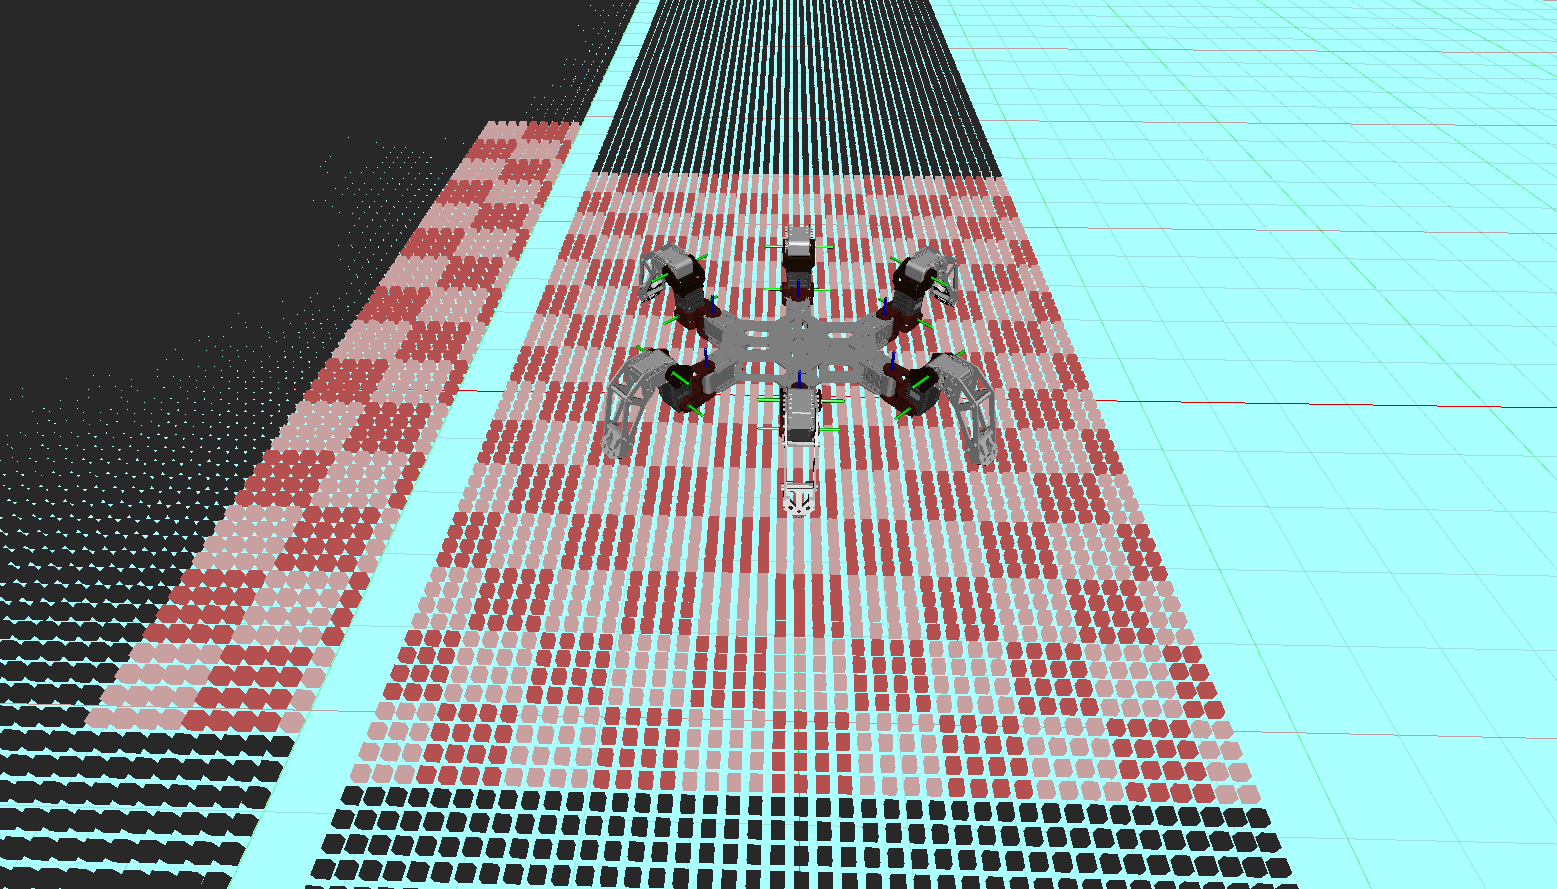
\includegraphics[width=80mm, clip]{figure/chapter3/map_view.png}
    \caption{Map View}
    \label{fig:map_view}  % chktex 24
  \end{center}
\end{figure}


\subsection{子ノードを作成するプログラム}
歩容パターングラフを作成するためには,子ノードを作成するプログラムが必要であり,
そのプログラムをINodeCreatorインターフェイスを実装した各クラスで実装している.
INodeCreatorインターフェイスは\figref{fig:node_creator_class_diagram}のように定義されている.
Create関数は,引数に現在のノード,現在のノードのインデックス,作成した子ノードを格納する配列へのポインタを持っている.
戻り値で結果を返す場合,RobotStateNode構造体のコピー処理が発生するため,
引数で渡した配列のポインタを通じて値を返している.
各クラスでは,Create関数をオーバーライドすることで,子ノードを作成する処理を実装している.

歩容パターングラフの規模を小さくするためには1つの親ノードがもつ子ノードの数は少なくする必要がある.
しかし,数を少なくしすぎると,グラフ探索によって必要な歩容パターンが消えてしまう可能性がある.
各クラスでは1つの親ノードから10個程度の子ノードを作成するようにしており,
深さ5の歩容パターングラフのノード数はが$10^5 \sim 10^6$程度となるようにしている.
ロボットの動作に応じて異なるクラスを用いたため,以下に各クラスの説明を記述する.
\\

% INodeCreator 構造体の説明
\begin{figure}[h]
  \centering
  \begin{tikzpicture}
    \begin{interface}[text width=7cm]{INodeCreator}{0, 0}
      \attribute{}
      \operation{+ Create(current\_node : RobotStateNode, current\_node\_index : int, 
                 output\_graph : std::vector~\textless~RobotStateNode~\textgreater~*) : void }
    \end{interface}
  \end{tikzpicture} 
  \caption{NodeCreator Interface}
  \label{fig:node_creator_class_diagram}  % chktex 24
\end{figure}

\subsubsection{重心の上下移動}
重心の上下移動を行うための処理はNodeCreatorComUpDownクラスで実装している.
NodeCreatorComUpDownクラスは処理を行うノードから,
重心を上下移動させることで作成できる子ノードを戻り値として返す.

重心の移動後の座標は無数に存在するため,\figref{fig:com_up_down}に離散化の様子を示した.
まず,現在の脚位置から下げることが可能な最低の重心高さと,
現在の脚位置から上げることが可能な最大の重心高さを計算する.
この時,近似された脚の可動範囲から脚先が届くかを判定しており,
またDevidedMapStateのdivided\_map\_top\_z\_を用いて,
地形との干渉を考慮している.
次に,最低の重心高さから最大の重心高さまで等間隔で5分割し,
各重心高さにおける子ノードを作成する.
重心の高さを変更しない場合を考慮して,そのままの重心高さを持つ子ノードも作成する.
離散化時の分割数はグラフの規模を考慮して決定した.

\begin{figure}[h]
  \begin{center}
    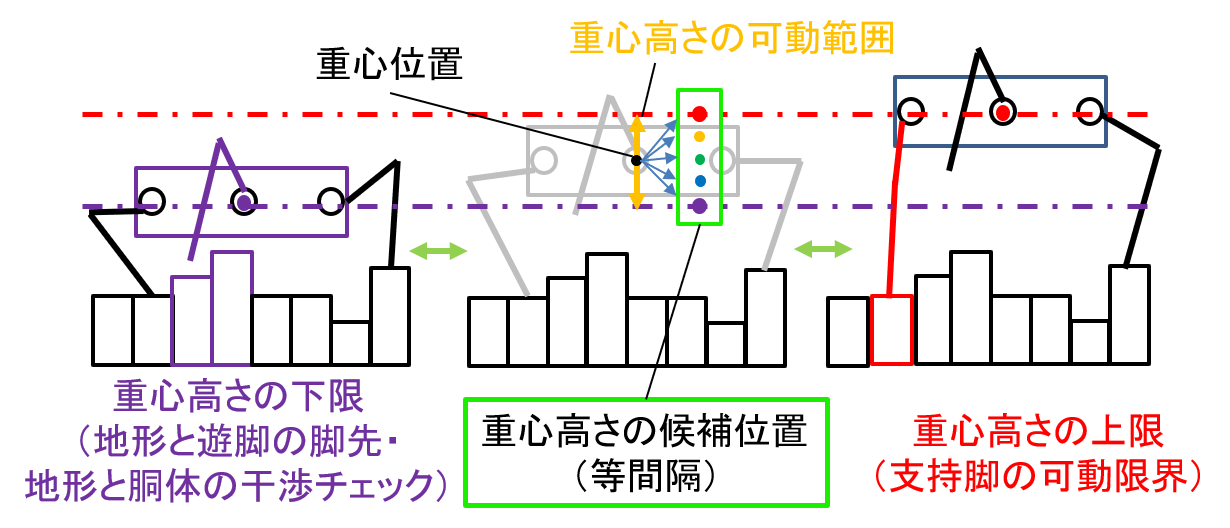
\includegraphics[width=70mm, clip]{figure/chapter3/com_up_down.png}
    \caption{Discretization of  \newline the Vertical Shift of the Center of Mass}
    \label{fig:com_up_down}  % chktex 24
  \end{center}
\end{figure}

\subsubsection{重心の平行移動}
重心の平行移動を行うための処理はNodeCreatorComMoveクラスで実装している.
NodeCreatorComMoveクラスは処理を行うノードから,
重心を平行移動させることで作成できる子ノードを戻り値として返す.

上下移動の場合と同様に,重心の移動後の座標は無数に存在するため以下の手順で離散化を行う.
まず重心を平行移動させる候補領域を\figref{fig:candidate_area_com}のように決定する.
脚先を投影してできる六角形の対角線をすべて結び,その交点から7通りの重心の候補領域を決定する.
そして,それぞれ右前方にあるものから順に1$\sim$6と番号を振る.
また,中央にあるもののうち,ロボットの前方を上としたときに逆三角形となるものを7,
ロボットの後方を上としたときに逆三角形となるものを8とする.

次にこれらの候補領域から実際に重心を平行移動させる地点を決定する.
\figref{fig:determination_of_com}に示すように,候補領域を格子状に分割する.
そして,各格子点において重心を平行移動させた時,
もっとも進行方向への移動量が大きくなる点を選択し子ノードの重心座標とする.
この時に静的安定余裕を確認し,規定された値を下回る場合はその点を選択しない.
また,このときRobotStateNode構造体のleg\_state\_の上位4bitに,
候補領域の番号を離散化された重心位置として格納する.
加えて,RobotStateNode構造体のleg\_reference\_pos\_を現在のleg\_pos\_の値に更新する.

\begin{figure}[h]
  \begin{tabular}{cc}
      \begin{minipage}{0.5\textwidth}
          \centering
          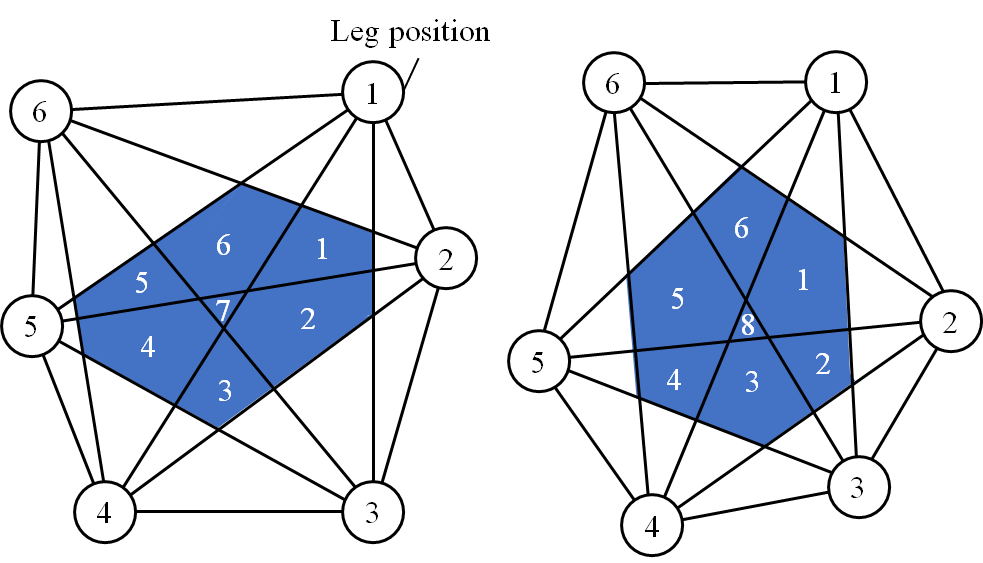
\includegraphics[width=1.0\linewidth]{figure/chapter3/leg_pos_com.png}
          \caption{Candidate Area of Center of Mass}
          \label{fig:candidate_area_com} % chktex 24
      \end{minipage}
      \begin{minipage}{0.5\textwidth}
          \centering
          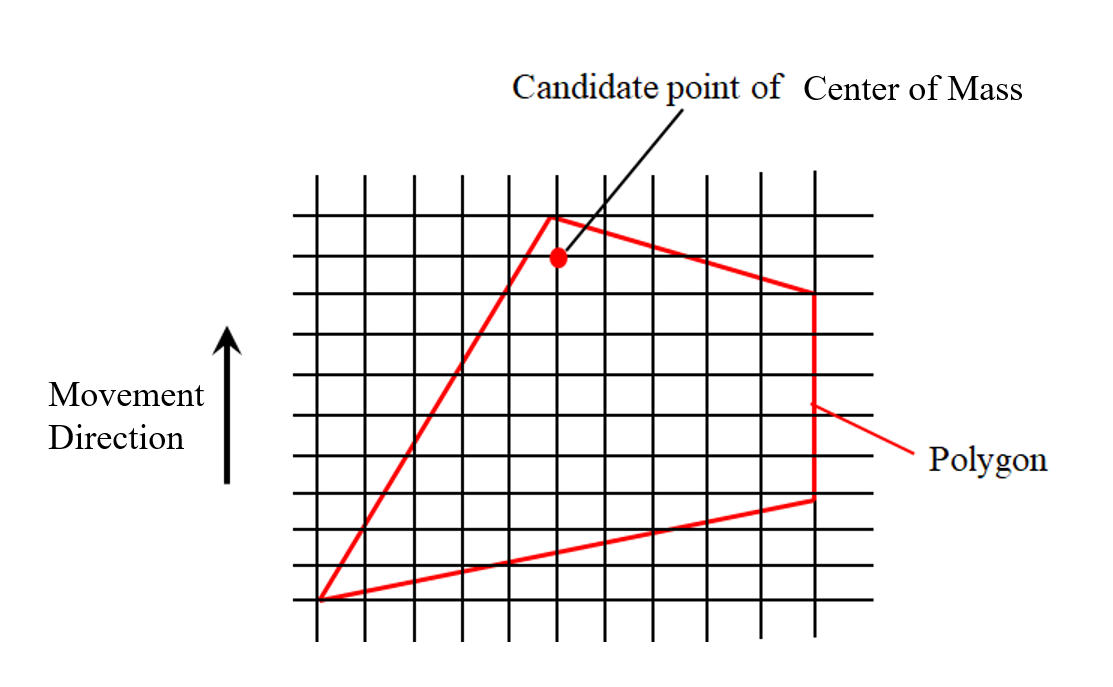
\includegraphics[width=1.0\linewidth]{figure/chapter3/center_of_mass.png}
          \caption{Determination of Center of Mass}
          \label{fig:determination_of_com} % chktex 24
      \end{minipage}
  \end{tabular}
\end{figure}

\subsubsection{胴体の回転移動}
胴体の回転運動を行うための処理はNodeCreatorBodyRotクラスで実装している.
NodeCreatorBodyRotクラスは処理を行うノードから,
胴体を回転させることで作成できる子ノードを戻り値として返す.

重心を中心として,重力の方向を軸とした回転運動を行う.
回転量は$-20 \sim 20 [\deg]$の範囲を$2 [\deg]$刻みで離散化しており,
1つのノードにつき21個の子ノードを作成する.
回転運動を行う際には,近似された脚の可動範囲から脚先が届くかを判定しており,
届かない場合,そのノードは作成しない.

\subsubsection{脚の上下運動・水平運動}
\chref{chapter:歩容パターンの再評価手法の提案}で述べたように,
脚の水平運動は脚の状態が等しく,別の階層にあるノード間での遷移で行うことができ,
脚の上下運動は同じ階層にあるノード間での遷移で行うことができる.
脚の状態が等しく,別の階層にある子ノードを生成する処理はNodeCreatorLegHierarchyクラスで実装しており,
同じ階層にある子ノードを生成する処理はNodeCreatorLegUpDownクラスで実装しているため,
まずは,NodeCreatorLegHierarchyクラスの説明を行う.

NodeCreatorLegHierarchyクラスでは,処理を行うノードの脚の状態を表すleg\_state\_から,
遊脚している脚を取得し,その脚の離散化された脚位置を$1 \sim 7$に変更した子ノードを作成する.
つまり1脚遊脚している場合は7つの子ノードを作成し,
3脚遊脚している場合は$7^3 = 343$の子ノードを作成する.
このクラスでは実際の脚位置を変更するのではなく,あくまで脚の状態を表すleg\_state\_を変更するのみである.

次にNodeCreatorLegUpDownクラスを説明する.
NodeCreatorLegUpDownクラスでは,処理を行うノードの脚の状態を表すleg\_state\_から,
遊脚の組み合わせを変更した子ノードを作成する.
遊脚の組み合わせのうち,接地しえない脚がある組み合わせは作成しないようにするため,
最初に現在遊脚中の各脚について,その脚が離散化された脚位置で指定された脚位置に接地することができるかを判定する.
また,重心の位置から静的安定性を保つことができない場合も作成しない.
処理の流れを以下に示す.

\begin{enumerate}
  \item 離散化された重心位置から同時に遊脚することができない隣り合う2脚を遊脚するノードを削除する\par
        RobotStateNodeのleg\_state\_から重心位置を取得し,
        その重心位置から同時に遊脚することができない隣り合う2つの脚を,
        同時に遊脚するノードを作成する候補から削除する.
        \tableref{tab:leg_combination_table}にある重心位置において,同時に遊脚することができない脚の組み合わせを示す.
        この表における重心位置や脚の番号は\figref{fig:candidate_area_com}のものと同じである.
  \item 離散化された脚位置で指定された位置に接地可能な点があるか確認する\par
        各脚ごとにRobotStateNodeのleg\_state\_から離散化された脚位置を取得し,
        その脚位置で指定された脚位置に接地可能な点があるかを確認する.
        接地可能な点がない場合,その脚を接地するノードを作成する候補から削除する.
        接地可能な点が複数ある場合はもっとも移動方向への移動量が大きくなる点を選択する.
  \item 子ノードを作成する\par
        (1)(2)の処理の中で候補から削除されなかった,階層内のノードを作成し,これらを子ノードとして返す.
\end{enumerate}

% 連続する2脚のうち,同時に遊脚することができない脚の組み合わせのテーブル
\begin{table}[h]
  \caption{Leg Combination Table}
  \label{tab:leg_combination_table}  % chktex 24
  \begin{center}
    \begin{tabular}{|c|c|c|} \hline  % chktex 44
      重心位置 & 遊脚可能な組 & 遊脚不可能な組  \\ \hline  % chktex 44
      1 & (3,4) (4,5) (5,6) & (6,1) (1,2) (2,3) \\ \hline  % chktex 44
      2 & (4,5) (5,6) (6,1) & (1,2) (2,3) (3,4) \\ \hline  % chktex 44
      3 & (5,6) (6,1) (1,2) & (2,3) (3,4) (4,5) \\ \hline  % chktex 44
      4 & (6,1) (1,2) (2,3) & (3,4) (4,5) (5,6) \\ \hline  % chktex 44
      5 & (1,2) (2,3) (3,4) & (4,5) (5,6) (6,1) \\ \hline  % chktex 44
      6 & (2,3) (3,4) (4,5) & (5,6) (6,1) (1,2) \\ \hline  % chktex 44
      7 & (2,3) (4,5) (6,1) & (1,2) (3,4) (5,6) \\ \hline  % chktex 44
      8 & (1,2) (3,4) (5,6) & (2,3) (4,5) (6,1) \\ \hline  % chktex 44
    \end{tabular}
  \end{center}
\end{table}

\subsubsection{直進動作時におけるノード生成の順番}
直進動作を行う時の,未探索のノードから遷移可能なノードをグラフに追加する際のルールについて説明する.
RobotStateNodeのnext\_move\_には,次の動作を表すHexapodMove型の変数が格納されている.
この変数の値によってどのNodeCreatorクラスを使用するかが決定される.
それぞれのNodeCreatorクラスは子ノードを作成する際に,
親ノードのnext\_move\_の値から子ノードのnext\_move\_の値を以下のルールに基づいて決定する.

\begin{itemize}
  \item 親ノード:脚の水平運動 → 子ノード:脚の上下運動
  \item 親ノード:脚の上下運動 → 子ノード:重心の上下移動
  \item 親ノード:重心の上下移動 → 子ノード:重心の平行移動
  \item 親ノード:重心の平行移動 → 子ノード:脚の水平運動
\end{itemize}

\noindent また,使用するNodeCreatorクラスは以下の4つである.

\begin{itemize}
  \item NodeCreatorLegUpDown
  \item NodeCreatorComUpDown
  \item NodeCreatorComMove
  \item NodeCreatorLegHierarchy
\end{itemize}

このようなルールを定めることによって明らかに無意味な動作
(たとえば,重心を上げる→重心を下げる動作を繰り返すものなど)
を生成することをあらかじめ防ぐことができる.
なお,直進動作以外の動作を行う場合は別のルールを用いてグラフを作成している.

\subsection{グラフ探索時のノードの評価方法}
グラフ探索時では歩容パターングラフのもっとも深いノードをすべて比較し,
最高評価となったノードへのパスから深さ1のノード次のノードとして返す.
RobotOperationで与えられた動作に対して,適切な動作を行うRobotStateNodeを評価するために,
グラフ探索時には複数のノードの評価項目がある.
IGraphSearcherを継承した具象クラスではノードを評価する関数を複数持っており,
それぞれの関数で評価項目を計算している.
この章では3次元空間の直進動作におけるノードの評価方法を説明する.

3次元空間の直進動作のグラフ探索はGraphSearcherStraightMoveクラスで実装している.
処理の流れを以下に示す.

\begin{enumerate}
  \item 高さの評価\par
        進行方向の地形の最大高さを確認し,その地点を歩行するために必要な最低の重心高さを求める.
        求めた重心高さと現在の重心高さの差を評価値として使用し,値が小さいほど評価を高くする,
        現在の最高評価ノードと比較して評価が高ければ最高評価ノードを更新する.
  \item 移動量の評価\par
        (1)が最大評価ノードと同じであれば,直進動作の移動量を評価する.
        まず,根ノードから評価を行うノードまでの移動量を計算する.
        目標方向と移動量の内積を計算し,その値が大きいほど評価を高くする.
        RobotOperationで目標位置が指定されている場合は,
        根ノードから目標位置までの移動ベクトルを正規化したものを目標方向として使用する.
        現在の最高評価ノードと比較して評価が高ければ最高評価ノードを更新する.        
  \item 脚の回転角度の平均値の評価\par
        (2)も最大評価ノードと同じであれば,脚の回転角度の平均値を評価する.
        根ノードと評価を行うノードの脚の回転角度の平均値を計算し,
        その値が大きいほど評価を高くする.
        現在の最高評価ノードと比較して評価が高ければ最高評価ノードを更新する.
\end{enumerate}

\section{歩容パターンの再評価手法の実装}
歩容パターンの再評価手法はIGaitPatternGeneratorインターフェイスを継承したクラスを作成することで実装できる.
IGaitPatternGeneratorインターフェイスを用いたことで,
デコレーターパターンを用いて容易に再評価手法を実装している.
デコレーターパターンとは,既存のクラスに新たな機能を追加するためのデザインパターンである.
デコレータ(デコレータパターンを用いて作られたクラス)はあるインターフェイスを継承するかつ,
自身と同じインターフェイスを継承したクラスをメンバ変数として持つ.
そしてメンバ関数を呼び出す際に,メンバ変数のメンバ関数と自身の持つ処理を実行することで,
既存のクラスをそのままに新たな機能を追加することができる.

再評価手法はGaitPatternGeneratorRevaluationクラスで実装されている.
GaitPatternGeneratorRevaluationクラスはIGaitPatternGeneratorインターフェイスを継承しており,
メンバ変数にIGaitPatternGeneratorインターフェイスのポインタを2つ持っている.
これらのポインタはコンストラクタで初期化され,
1つ目のポインタは再評価手法を適用する前の歩容パターン生成手法を,
2つ目のポインタは再評価手法を適用した後の歩容パターン生成手法を指している.

メンバ関数であるGetNextNodeByGraphSearch関数が呼ばれた場合,
まず,1つ目のポインタのGetNextNodeByGraphSearch関数を呼び出し結果を取得する.
取得したノードから脚軌道生成を行い,成功した場合はそのノードを返す.
失敗した場合は,2つ目のポインタのGetNextNodeByGraphSearch関数を呼び出し結果を取得する.
こうすることで,\chref{chapter:歩容パターンの再評価手法の提案}で提案した,
脚軌道生成に失敗した場合のみグラフ探索をやり直す処理を実装できる.

再評価時には脚軌道生成の失敗を防ぐために,近似された脚の可動範囲を狭める.
近似された脚の可動範囲は\chref{chapter:歩容パターンの再評価手法の提案}で述べたように,
最小半径を$140 [mm]$に設定すればよいため,
狭めた前と後の脚の可動範囲は以下のような条件に設定する.
また,それぞれを図示したものを\figref{fig:leg_range_revaluation_before}と
\figref{fig:leg_range_revaluation_after}に示す.

\begin{enumerate}
  \item 再評価前\par
        \begin{itemize}
          \item 最小半径を$130 [mm]$に設定
          \item 最大半径は\chref{chapter:歩容パターンの再評価手法の提案}で述べた計算方法で設定
          \item 遊脚高さは$-20 [mm]$に設定
        \end{itemize}
  \item 再評価後\par
        \begin{itemize}
          \item 最小半径を$140 [mm]$に設定
          \item 最大半径は\chref{chapter:歩容パターンの再評価手法の提案}で述べた計算方法で設定
          \item 遊脚高さは$-20 [mm]$に設定
        \end{itemize}
\end{enumerate}

\begin{figure}[htbp]
  \centering
  \begin{tikzpicture}  % [show background grid]
    \begin{interface}[text width=70mm]{IGaitPatternGenerator}{-9, -7}
      \attribute{}
      \operation{}
    \end{interface}

    \begin{class}[text width=70mm]{GaitPatternGeneratorRevaluation}{-12, -2}
      \inherit{IGaitPatternGenerator}
      \attribute{- gait\_pattern\_generator\_ptr\_ : std::unique\_ptr\textless~IGaitPatternGenerator~\textgreater}
      \attribute{- gait\_pattern\_generator\_revaluation\_ptr\_ : std::unique\_ptr\textless~IGaitPatternGenerator~\textgreater}
      \operation{}
    \end{class}

    \begin{class}[text width=50mm]{GaitPatternGeneratorBasic}{-5.5, -4}
      \inherit{IGaitPatternGenerator}
      \attribute{}
      \operation{}
    \end{class}

  \end{tikzpicture}
  \caption{Gait Pattern Generator Revaluation Class Diagram}
  \label{fig:gait_pattern_generator_revaluation}  % chktex 24
\end{figure}

\begin{figure}[h]
  \begin{tabular}{cc}
      \begin{minipage}{0.5\textwidth}
          \centering
          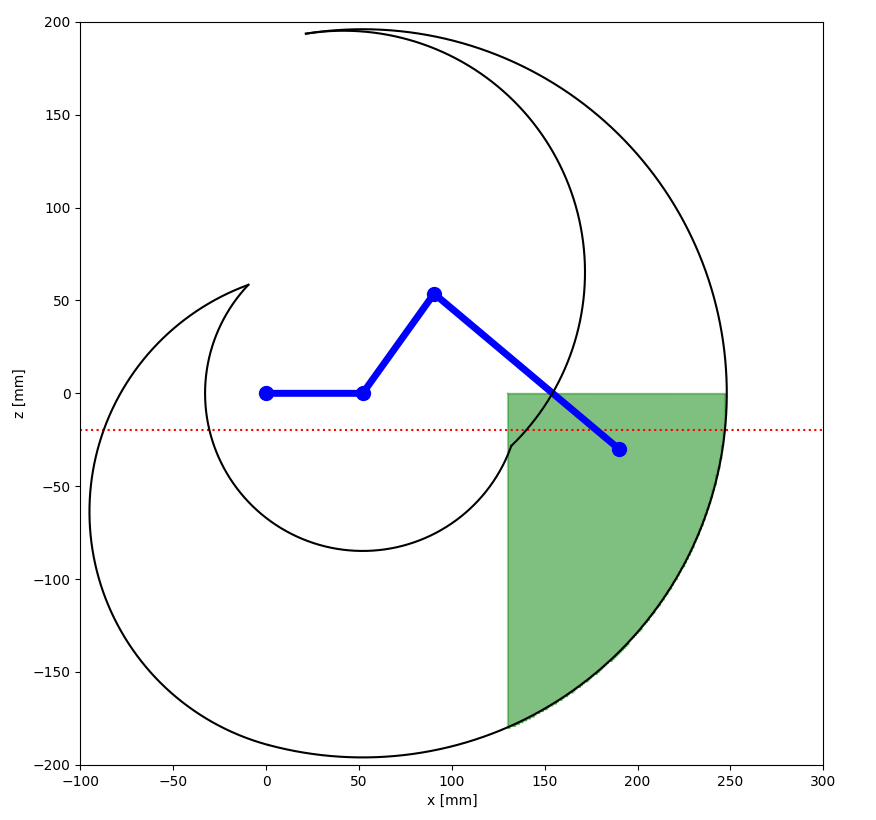
\includegraphics[width=1.0\linewidth]{figure/chapter3/revaluetion_before.png}
          \caption{Leg Range Before Revaluation}
          \label{fig:leg_range_revaluation_before} % chktex 24
      \end{minipage}
      \begin{minipage}{0.5\textwidth}
          \centering
          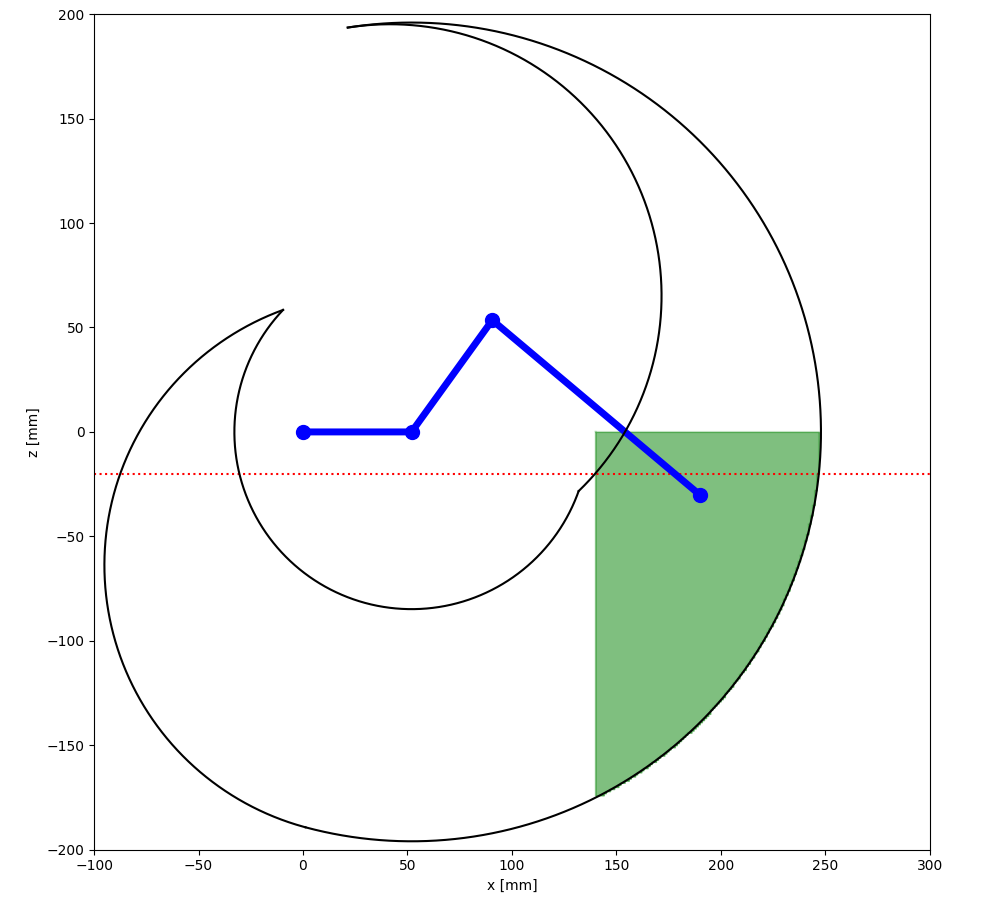
\includegraphics[width=1.0\linewidth]{figure/chapter3/revaluetion_after.png}
          \caption{Leg Range After Revaluation}
          \label{fig:leg_range_revaluation_after} % chktex 24
      \end{minipage}
  \end{tabular}
\end{figure}

\newpage

\section{グラフ探索による自由歩容パターン生成手法の統合}
先行研究において,グラフ探索による自由歩容パターン生成手法はロボットの動作によって別のものを使用しており,
それぞれ別のプログラムで実装されている.
しかし,不整地の踏破を行うためには,さまざまな動作を組み合わせて使用する必要がある.
より柔軟な動作をグラフ探索による自由歩容パターン生成手法で実現するため,
グラフ探索による自由歩容パターン生成手法を統合し,1つのプログラムで実行できるようにした.

この作業は本研究の趣旨とは異なるが,
直進以外のさまざまな動作でも脚軌道生成の失敗を防ぐことができるかを確認することができれば,
再評価手法がより汎用的なものであることを示すことができると考え,本作業を実施した.

\subsection{3次元空間における旋回動作の実装}
先行研究において,すでに実装されているロボットの動作を\tableref{tab:implemented_robot_operation}に示す.
表において,2次元空間とはロボットが平面上で動作することを表し,
3次元空間とはロボットが立体的な地形で動作することを表す.
また,$\bigcirc$がついている動作は実装済みであることを表し,
$\times$がついている動作は未実装であることを表す.
この表より,3次元空間における動作は直進以外実装されていないことがわかる.
より柔軟な動作を実現するという目的のもとでは,
統合されたプログラムは3次元空間に対応していることが望ましい.
よって3次元空間における旋回動作を実装した.

旋回動作の研究は椎名ら\cite{Shina_Graph_search}によって行われており,
旋回の半径によって異なる歩容パターングラフの作成と,グラフ探索が行われていた.
今回は簡単のため,旋回の半径が$0 [mm]$である場合(超信地旋回的に旋回を行う場合)のみを対象とし,
以降,旋回と記述するときはそのような旋回を指すものとする.

GaitPatternGeneratorRevaluationクラスを用いて再評価手法を実装することを考えると,
旋回動作時においてもGaitPatternGeneratorBasicクラスを用いることが望ましい.
ノードを生成する処理はINodeCreatorインターフェイスを継承した具象クラスによって実装されており,
グラフ探索を行う処理はIGraphSearcherインターフェイスを継承した具象クラスによって実装されている.
よってこれらのクラスを旋回動作用に作成することで,旋回動作時においても
GaitPatternGeneratorBasicクラスを用いることができる.
以下にそれぞれの実装を説明する.

\begin{table}[htbp]
	\caption{Implemented Robot Operation}
	\label{tab:implemented_robot_operation}  % chktex 24
	\begin{center}
   	\begin{tabular}{|c|c|c|c|c|c|c|} \hline  % chktex 44
    	\backslashbox{動作}{ロボット} & 2次元空間 & 3次元空間  \\ \hline  % chktex 44
      直進 & $\bigcirc$ & $\bigcirc$ \\ \hline  % chktex 44
      その場旋回 & $\bigcirc$ & $\times$ \\ \hline  % chktex 44
      旋回 & $\bigcirc$ & $\times$ \\ \hline  % chktex 44
      特定姿勢での静止 & $\bigcirc$ & $\times$ \\ \hline  % chktex 44
      %% まるはtexにおいて,$\bigcirc$
      %% ばつはtexにおいて,$\times$
    \end{tabular}
  \end{center}
\end{table}

\subsubsection{旋回動作時におけるノード生成の順番}
旋回動作時は胴体を平行移動させる必要がないため,
胴体平行移動を行うノードを生成しないようにする.
胴体平行移動を行う処理を,胴体の回転運動を行うノードを生成する処理に変更した.
旋回動作時のノード生成の順番は以下のように定める.

\begin{itemize}
  \item 親ノード:脚の水平運動 → 子ノード:脚の上下運動
  \item 親ノード:脚の上下運動 → 子ノード:重心の上下運動
  \item 親ノード:重心の上下運動 → 子ノード:胴体の回転運動
  \item 親ノード:胴体の回転運動 → 子ノード:脚の水平運動
\end{itemize}

また,使用するNodeCreatorクラスは以下の4つである.

\begin{itemize}
  \item NodeCreatorLegUpDown
  \item NodeCreatorComUpDown
  \item NodeCreatorComMove
  \item NodeCreatorLegHierarchy
\end{itemize}

\subsubsection{旋回動作時におけるノードの評価方法}
3次元空間における旋回動作のグラフ探索はGraphSearcherSpotTurnクラスで実装している.
処理の流れを以下に示す.

\begin{enumerate}
  \item 高さの評価\par
    進行方向の地形の最大高さを確認し,
    その地点を歩行するために必要な最低の重心高さを求める.
    求めた重心高さと現在の重心高さの差を評価値として使用し,
    値が小さいほど評価を高くする,
    現在の最高評価ノードと比較して評価が高ければ最高評価ノードを更新する.
  \item 回転量の評価\par
    (1)が最大評価ノードと同じであれば旋回動作の回転量を評価する.
    RobotOperationで指定された姿勢を目標姿勢とし,
    評価を行うノードの姿勢と目標姿勢との角度の差を評価値として使用する.
    現在の最高評価ノードと比較して評価が高ければ最高評価ノードを更新する.
  \item 脚の回転角どの平均値の評価\par
    (2)も最大評価ノードと同じであれば,脚の回転角度の平均値を評価する.
    根ノードと評価を行うノードの脚の回転角度の平均値を計算し,
    その値が大きいほど評価を高くする.
    現在の最高評価ノードと比較して評価が高ければ最高評価ノードを更新する.
\end{enumerate}

\subsection{自由歩容パターン生成手法を切り替えるクラスの実装}
グラフ探索による自由歩容パターン生成手法を統合するために,
1つの歩容パターングラフにさまざまな動作を行うためのノードを追加することを考える.
この場合,歩容パターングラフのノードの数が増えるため処理にかかる時間が増加する.
また,作成される歩容パターングラフの内容が変化してしまうため,
すでに開発されたグラフ探索手法に影響を及ぼす可能性がある.
いままでに動作によって異なるプログラムを用いていたことからも,
ロボットの動作によって使用する自由歩容パターン生成手法を切り替えることで,
1つのプログラムに統合する手法が適していると考えた.
以下に自由歩容パターン生成手法を切り替えるクラスの実装方法を示す.


 % 第3章
    

\chapter{再評価手法の有効性の確認のための歩行シミュレーション}\label{chapter:再評価手法の有効性の確認のための歩行シミュレーション}
第\ref{chapter:再評価手法の有効性の確認のための歩行シミュレーション}章では,
実装した再評価手法の有効性を確認するために,シミュレーションを用いた歩行実験を行い,その結果を示す.

\section{直進動作の自由歩容パターン生成シミュレーション}
まずは,直進動作の自由歩容パターン生成シミュレーションを行い,再評価手法の有効性を確認する.

\subsection{シミュレーション実験の目的}
シミュレーション実験の目的は,
再評価手法によって生成された自由歩容パターンを用いて,
脚軌道生成の失敗が生じないことを確認することとする.

波東らの研究で実機では歩行することができなかった地形を含む5種類の地形を歩行させ,
脚軌道生成の失敗の回数が0回となることを確認する.
また再評価手法の利点として,計算時間が大幅に伸びないことが期待されるため,計算にかかる時間も測定する.

\subsection{シミュレーション実験の条件}
シミュレーションには,\chref{chapter:歩容パターンの再評価手法の提案}で使用したシミュレーションソフトウェアを使用した.
また,計算環境も同じく\tableref{tab:simulation_env}に示したものを用いており,
シミュレーションのモデルとしたロボットも同じくPhantomXとした.

\subsubsection{歩行する地形}
シミュレーションに使用する地形を\figref{fig:ch5_simu_terrain}に示す.
また矢印でロボットの進行方向を示した.
シミュレーションに使用した地形は,平面,130mmの上り段差,130mmの下り段差,15度の上り斜面,15度の下り斜面の5種類である.
\chref{chapter:歩容パターンの再評価手法の提案}で行ったシミュレーションの条件から変更し,上り段差と下り段差の高さを130mmとしている.

\subsubsection{歩行する時の条件}
シミュレーション時の歩行条件は以下の通りである.
\begin{itemize}
  \item 胴体姿勢は常に水平である.
  \item 最小半径を$130 [mm]$とし,再評価時には最小半径を$140 [mm]$に変更する.
  \item 重心から見た遊脚高さを$-20 [mm]$とする.
  \item 胴体を地形から最小$30 [mm]$離す.
  \item 常に静的安定余裕は$15 [mm]$以上を保つ.
\end{itemize}

\subsubsection{シミュレーションの手順}
各地形で水平方向に$1200 [mm]$直進するまでの自由歩容パターンを生成した.
\figref{fig:ch5_simu_terrain}のロボットの初期位置をランダムに変化させて計5回ずつ歩行させた.
再評価手法を用いた場合と用いていない場合を比較するため,
再評価手法を用いず初めから最小半径を$140 [mm]$としたプログラムを用いて同様のシミュレーションを行った.
シミュレーションごとに,脚軌道生成の失敗の回数,脚先座標,計算時間を測定した.

% 地形の図
\begin{figure}[tb]
  \begin{tabular}{cc}
    \begin{minipage}[t]{0.45\hsize}
      \begin{center}
      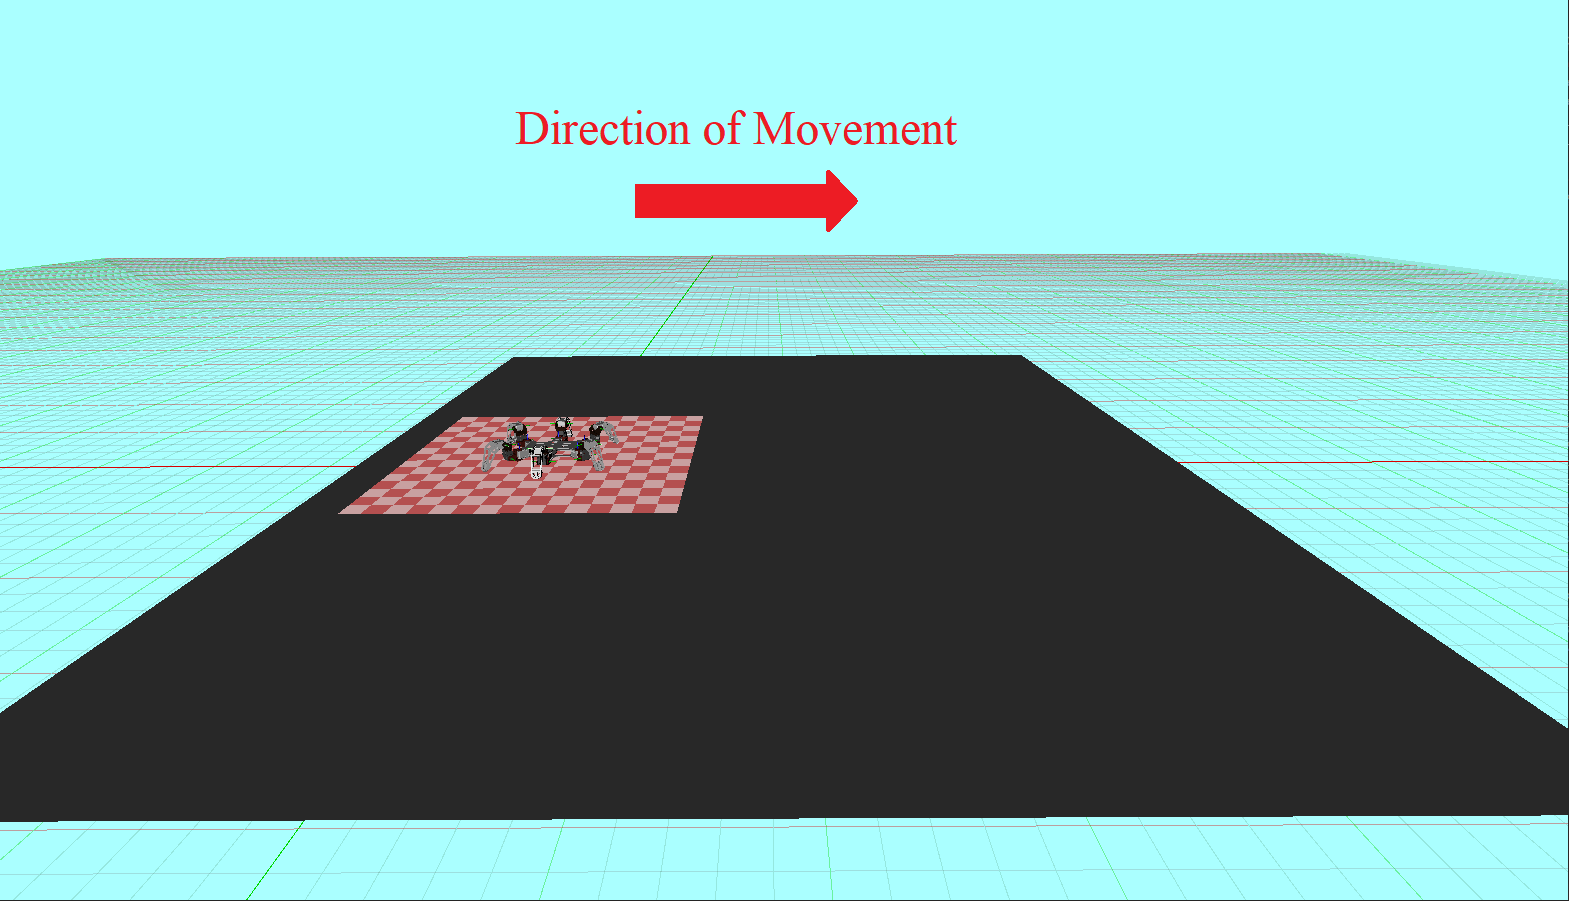
\includegraphics[width=1.0\linewidth]{figure/chapter4/map_flat.png}
      \text{(a) flat}
      \label{fig:ch5_simu_terrain_flat} % chktex 24
      \end{center}
    \end{minipage} 
    &
    \begin{minipage}[t]{0.45\hsize}
      \begin{center}
      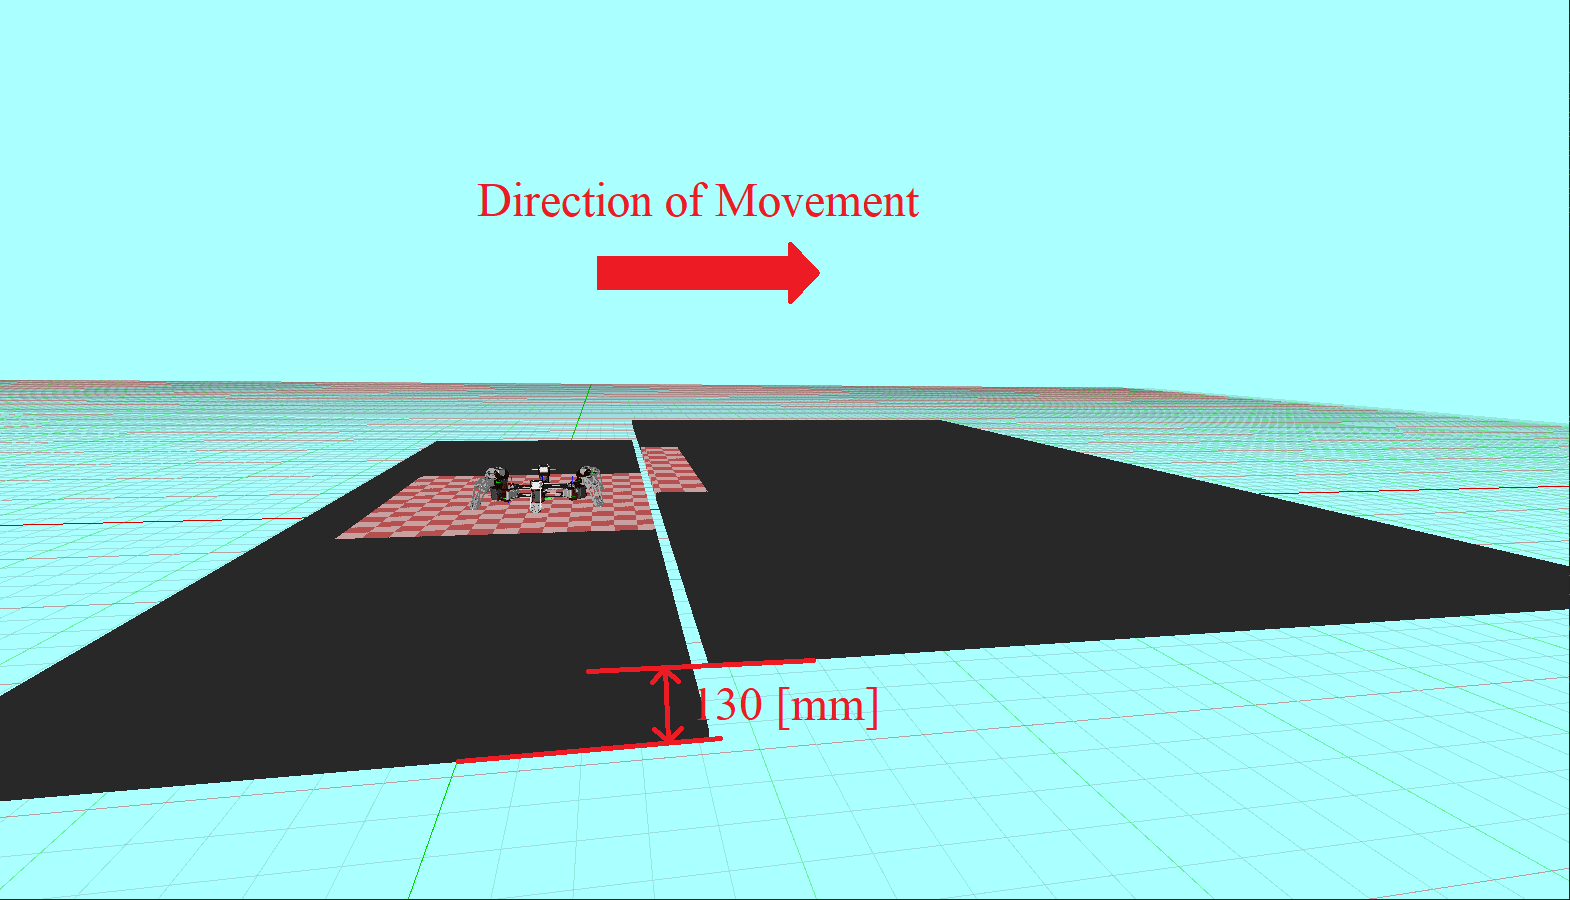
\includegraphics[width=1.0\linewidth]{figure/chapter4/map_130mm.png}
      \text{(b) up step}
      \label{fig:ch5_simu_terrain_up_step} % chktex 24
      \end{center}  
    \end{minipage}
    \\
    &\\  % 空白を入れる
    \begin{minipage}[t]{0.45\hsize}
      \centering
      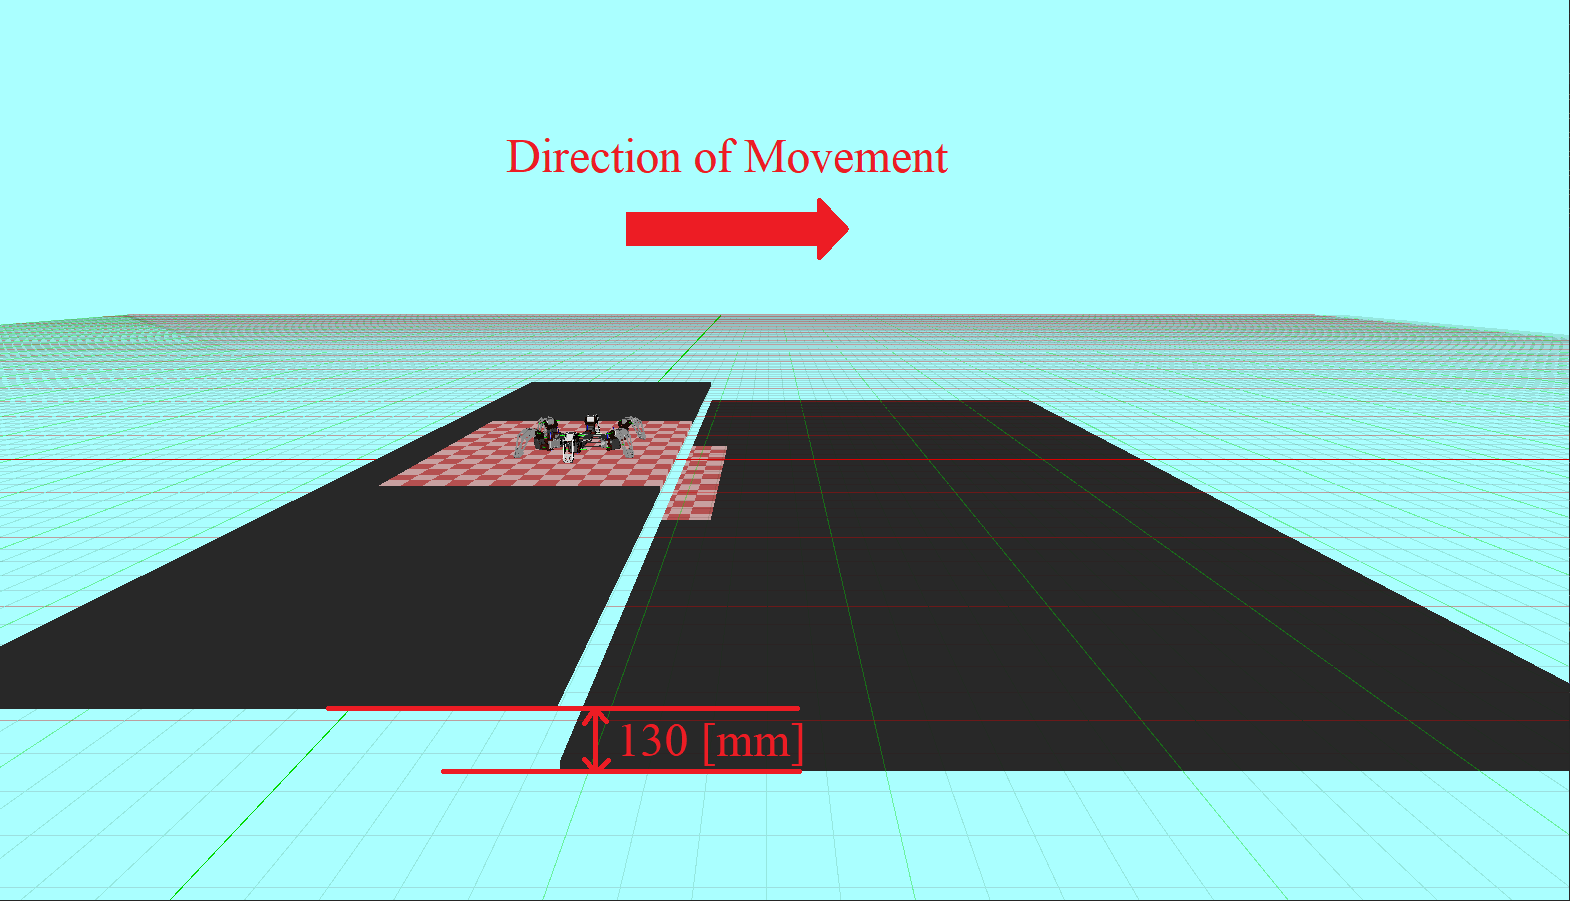
\includegraphics[width=1.0\linewidth]{figure/chapter4/map_-130mm.png}
      \centering
      \text{(c) down step}
      \label{fig:ch5_simu_terrain_down_step} % chktex 24
    \end{minipage} 
    &
    \begin{minipage}[t]{0.45\hsize}
      \centering
      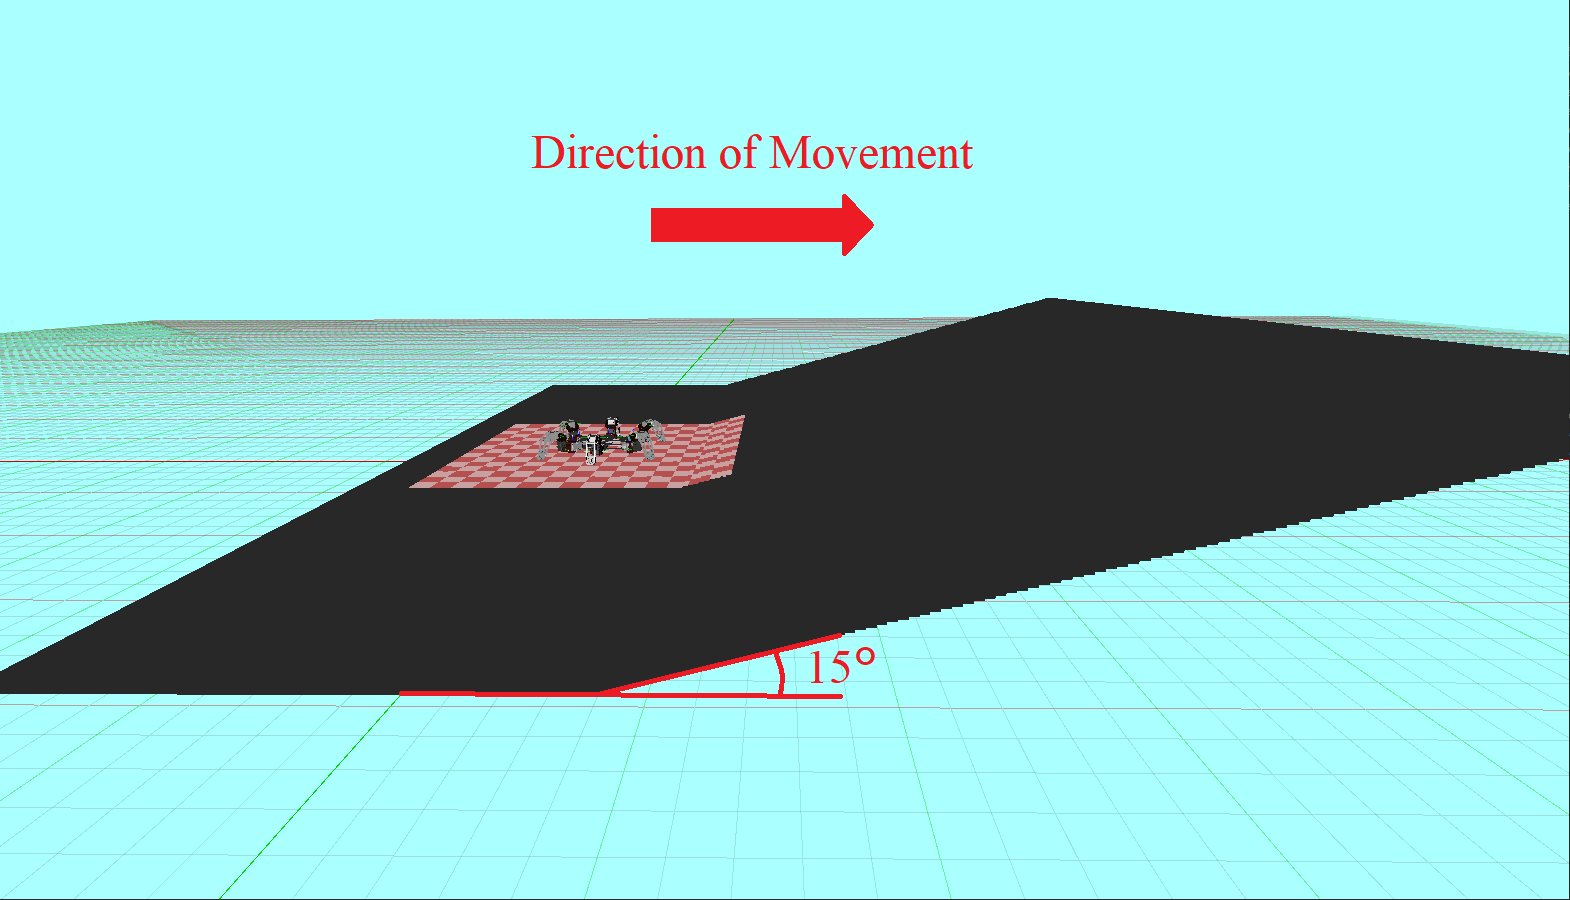
\includegraphics[width=1.0\linewidth]{figure/chapter4/map_15deg.png}
      \centering
      \text{(d) up slope}
      \label{fig:up_slope_terrain} % chktex 24
    \end{minipage}    
    \\
    &\\  % 空白を入れる
    \begin{minipage}[t]{0.45\hsize}
      \centering
      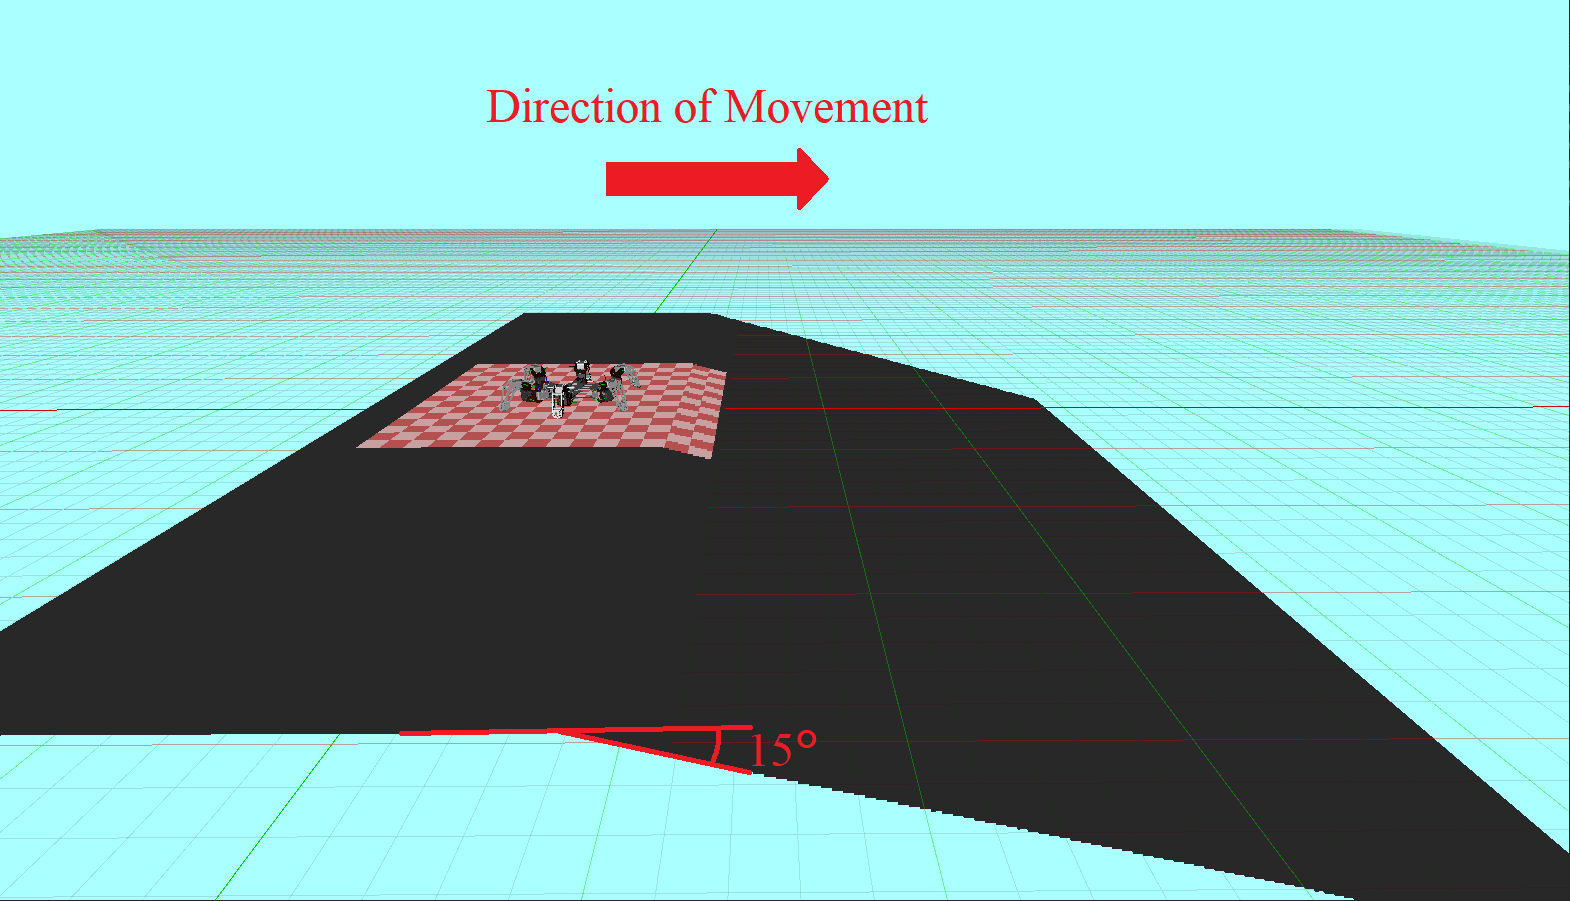
\includegraphics[width=1.0\linewidth]{figure/chapter4/map_-15deg.png}
      \centering
      \text{(e) down slope}
      \label{fig:down_slope_terrain} % chktex 24
    \end{minipage}     
    &
    \\
  \end{tabular}
  \caption{Terrain}
  \label{fig:ch5_simu_terrain} % chktex 24
\end{figure}

\newpage

\subsection{シミュレーション実験の結果}
\subsubsection{脚軌道生成の失敗の回数}
再評価手法を用いた場合の脚軌道生成の失敗の回数を\tableref{tab:ch5_failure_count_1}に示す.
また,再評価手法を用いない場合の脚軌道生成の失敗の回数を\tableref{tab:ch5_failure_count_2}に示す.
この結果から,再評価手法を用いた場合でも,脚軌道生成の失敗が生じてしまうことがわかる.
失敗する場合は,遊脚時に脚軌道が可動範囲外を通ることがわかる.
加えて,初めから最小半径を140mmとすれば,脚軌道生成の失敗は生じていないことがわかる.

\begin{table}[tb]
  \caption{Failure Count of Revaluation}
  \label{tab:ch5_failure_count_1}  % chktex 24
  \small
  \centering
  \begin{tabular}{|c|c|c|c|c|c|c|c|} \hline  % chktex 44
    \multirow{3}{*}{地形} & \multirow{3}{*}{グラフ探索} & \multicolumn{5}{c|}{失敗の回数} & \multirow{3}{*}{失敗率 $[\%]$} \\ \cline{3-7}  % chktex 44
     & & \multirow{2}{*}{脚接地点が} & \multicolumn{3}{c|}{脚軌道が可動範囲外を通る} & \multirow{2}{*}{総失敗} & \\ \cline{4-6}  % chktex 44
     & の回数 & 可動範囲外 & 遊脚時 & 接地時 & \begin{tabular}{c}胴体平行\\移動時\end{tabular} & 回数 & \\ \hline  % chktex 44
    平面     & 340 & 0 & 21 & 0 & 0 & 0 & 6.17 \\ \hline  % chktex 44
    上り斜面 & 700 & 0 & 35 & 0 & 0 & 0 & 5.00 \\ \hline  % chktex 44
    下り斜面 & 712 & 0 & 18 & 0 & 0 & 0 & 2.52 \\ \hline  % chktex 44
    上り段差 & 500 & 0 & 21 & 0 & 0 & 0 & 4.20 \\ \hline  % chktex 44
    下り段差 & 640 & 0 & 34 & 0 & 0 & 0 & 5.31 \\ \hline  % chktex 44
  \end{tabular}
\end{table}

\begin{table}[tb]
  \caption{Failure Count of Revaluation}
  \label{tab:ch5_failure_count_2}  % chktex 24
  \small
  \centering
  \begin{tabular}{|c|c|c|c|c|c|c|c|} \hline  % chktex 44
    \multirow{3}{*}{地形} & \multirow{3}{*}{グラフ探索} & \multicolumn{5}{c|}{失敗の回数} & \multirow{3}{*}{失敗率 $[\%]$} \\ \cline{3-7}  % chktex 44
     & & \multirow{2}{*}{脚接地点が} & \multicolumn{3}{c|}{脚軌道が可動範囲外を通る} & \multirow{2}{*}{総失敗} & \\ \cline{4-6}  % chktex 44
     & の回数 & 可動範囲外 & 遊脚時 & 接地時 & \begin{tabular}{c}胴体平行\\移動時\end{tabular} & 回数 & \\ \hline  % chktex 44
    平面     & 389 & 0 & 0 & 0 & 0 & 0 & 0 \\ \hline  % chktex 44
    上り斜面 & --- & 0 & 0 & 0 & 0 & 0 & 0 \\ \hline  % chktex 44
    下り斜面 & 689 & 0 & 0 & 0 & 0 & 0 & 0 \\ \hline  % chktex 44
    上り段差 & 513 & 0 & 0 & 0 & 0 & 0 & 0 \\ \hline  % chktex 44
    下り段差 & 681 & 0 & 0 & 0 & 0 & 0 & 0 \\ \hline  % chktex 44
  \end{tabular}
\end{table}

\subsubsection{脚先座標}
再評価手法を用いた場合の,脚先座標を地形ごとに以下の図で示した.
脚先座標は支持脚時を青い丸点,遊脚時を赤い丸点で示している.
また,脚軌道生成に失敗した際の脚軌道の中継点を水色の$\times$で示している.


\begin{figure}[htbp]
  \begin{tabular}{cc}
    \begin{minipage}[t]{0.41\hsize}
      \begin{center}
      \includegraphics[width=1.0\linewidth,trim={30 30 30 30}, clip]{figure/chapter4/revaluation/flat.png}
      \text{(a) flat terrain}
      \end{center}
    \end{minipage} 
    &
    \begin{minipage}[t]{0.41\hsize}
      \begin{center}
      \includegraphics[width=1.0\linewidth,trim={30 30 30 30}, clip]{figure/chapter4/revaluation/130mm.png}
      \text{(b) up step terrain}
      \end{center}  
    \end{minipage}
    \\
    \begin{minipage}[t]{0.41\hsize}
      \centering
      \includegraphics[width=1.0\linewidth,trim={30 30 30 30}, clip]{figure/chapter4/revaluation/-130mm.png}
      \centering
      \text{(c) down step terrain}
    \end{minipage} 
    &
    \begin{minipage}[t]{0.41\hsize}
      \centering
      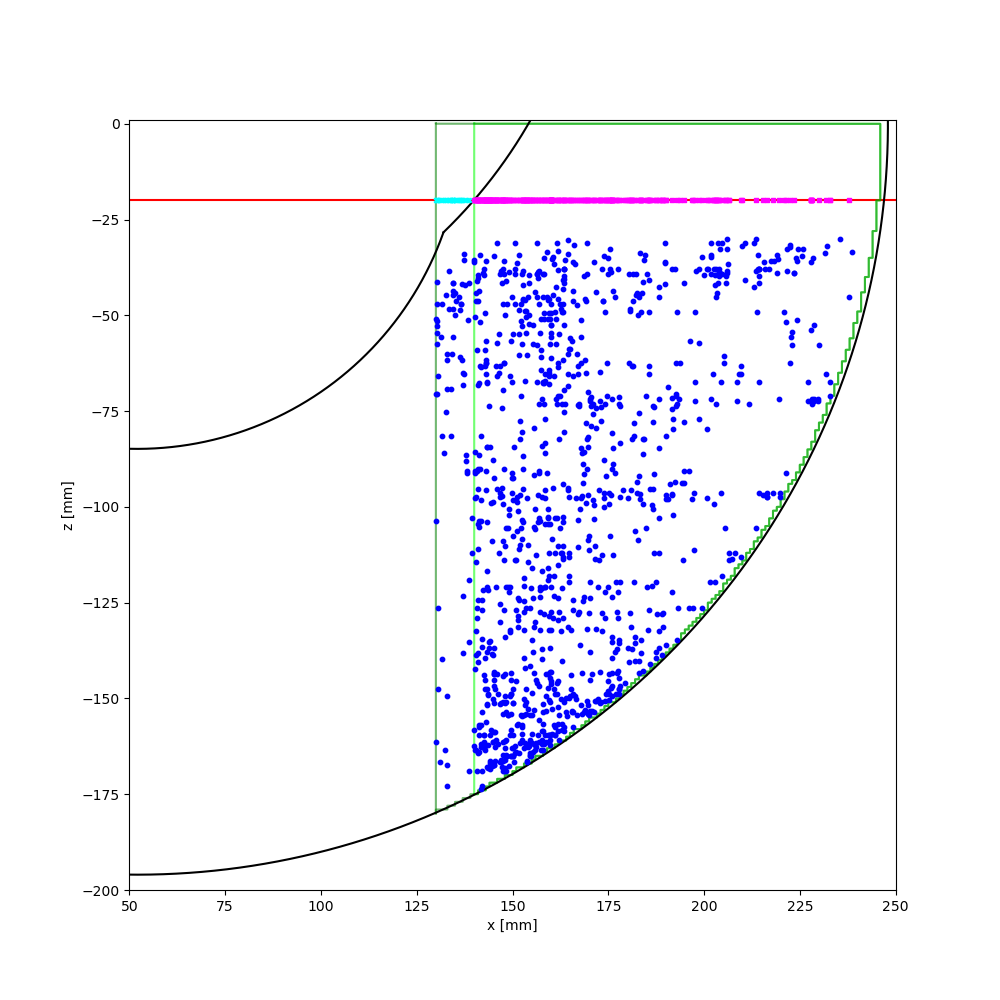
\includegraphics[width=1.0\linewidth,trim={30 30 30 30}, clip]{figure/chapter4/revaluation/15deg.png}
      \centering
      \text{(d) up slope terrain}
    \end{minipage}    
    \\
    \begin{minipage}[t]{0.41\hsize}
      \centering
      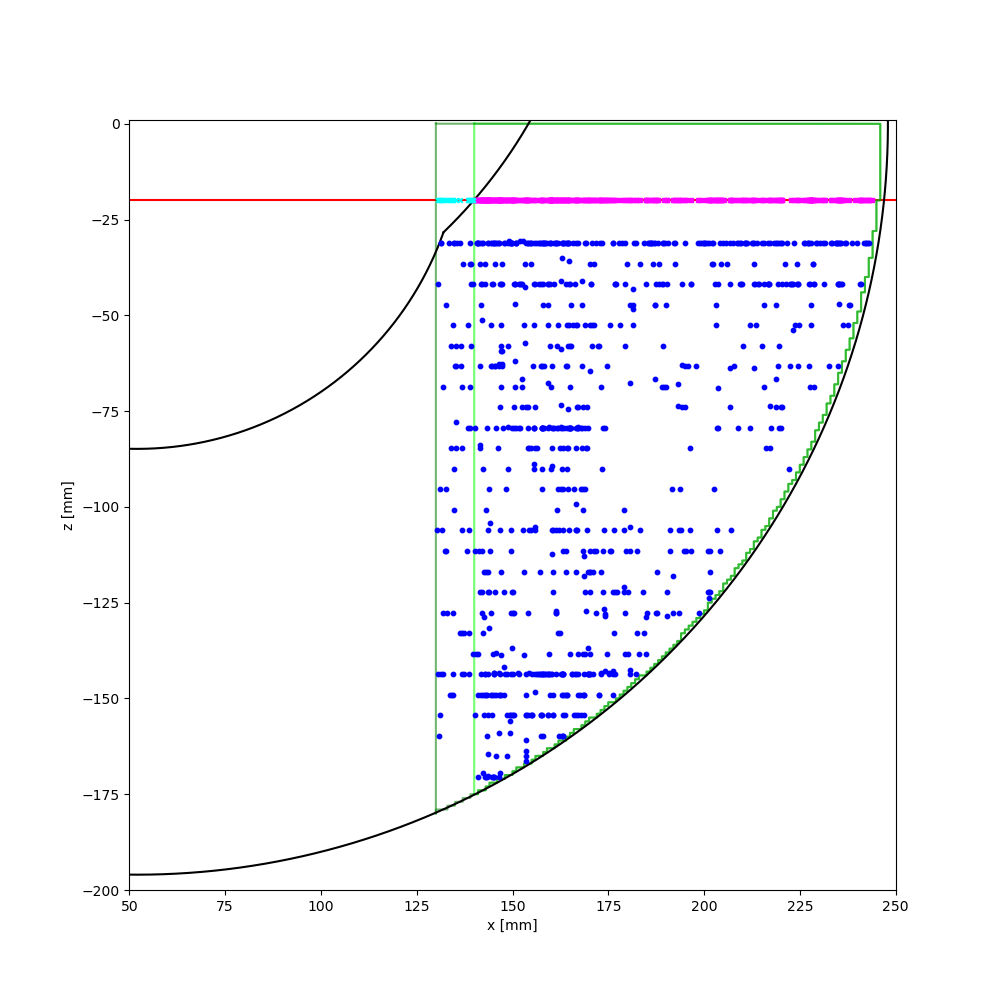
\includegraphics[width=1.0\linewidth,trim={30 30 30 30}, clip]{figure/chapter4/revaluation/-15deg.png}
      \centering
      \text{(e) down slope terrain}
      
    \end{minipage}     
    &
    \\
  \end{tabular}
  \caption{Leg Ground Points for each Terrain (when Revaluation Method)}
  \label{fig:ch5_simu_res_1} % chktex 24
\end{figure}


\begin{figure}[htbp]
  \begin{tabular}{cc}
    \begin{minipage}[t]{0.41\hsize}
      \begin{center}
      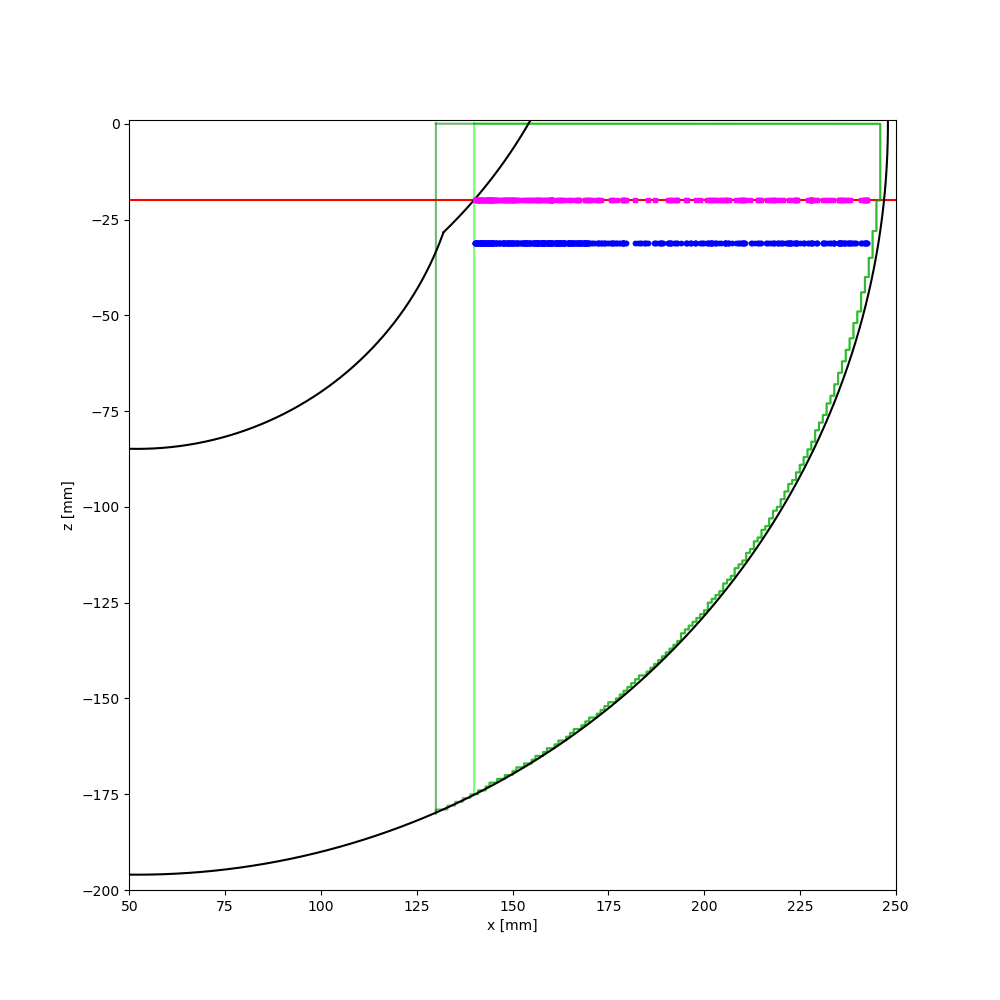
\includegraphics[width=1.0\linewidth,trim={30 30 30 30}, clip]{figure/chapter4/140mm/flat.png}
      \text{(a) flat terrain}
      \end{center}
    \end{minipage} 
    &
    \begin{minipage}[t]{0.41\hsize}
      \begin{center}
      \includegraphics[width=1.0\linewidth,trim={30 30 30 30}, clip]{figure/chapter4/140mm/130mm.png}
      \text{(b) up step terrain}
      \end{center}  
    \end{minipage}
    \\
    \begin{minipage}[t]{0.41\hsize}
      \centering
      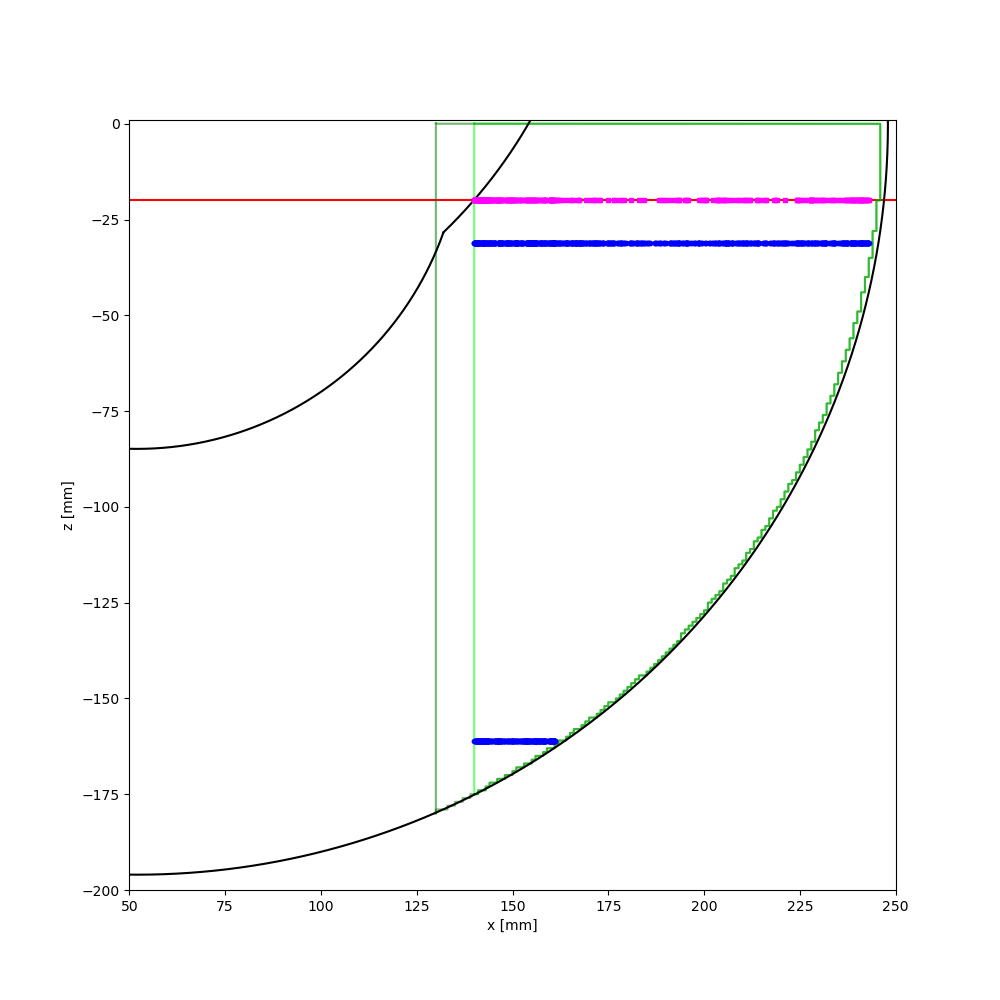
\includegraphics[width=1.0\linewidth,trim={30 30 30 30}, clip]{figure/chapter4/140mm/-130mm.png}
      \centering
      \text{(c) down step terrain}
    \end{minipage} 
    &
    \begin{minipage}[t]{0.41\hsize}
      \centering
      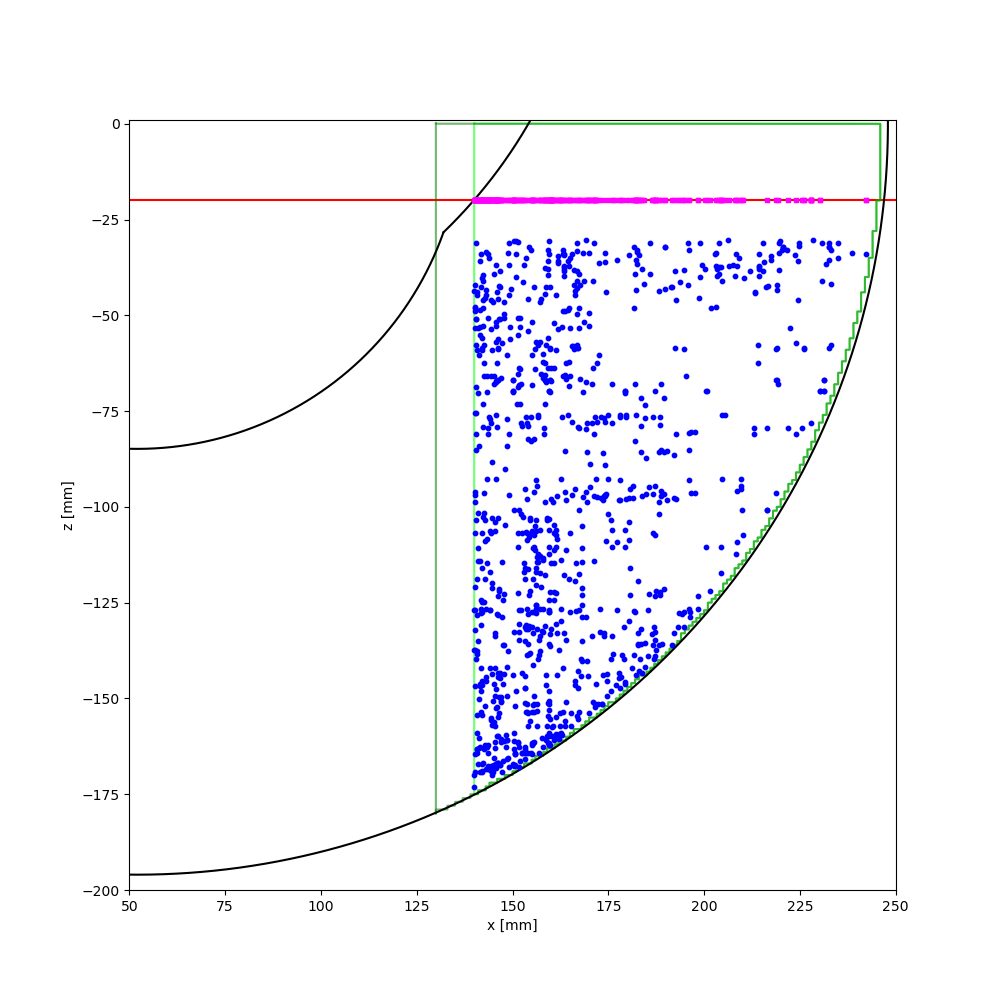
\includegraphics[width=1.0\linewidth,trim={30 30 30 30}, clip]{figure/chapter4/140mm/15deg.png}
      \centering
      \text{(d) up slope terrain}
    \end{minipage}    
    \\
    \begin{minipage}[t]{0.41\hsize}
      \centering
      \includegraphics[width=1.0\linewidth,trim={30 30 30 30}, clip]{figure/chapter4/140mm/-15deg.png}
      \centering
      \text{(e) down slope terrain}
      
    \end{minipage}     
    &
    \\
  \end{tabular}
  \caption{Leg Ground Points for each Terrain (without Revaluation Method)}
  \label{fig:ch5_simu_res_2} % chktex 24
\end{figure}

\newpage


\subsubsection{計算時間}
再評価手法を用いた場合の1つの動作生成にかかる計算時間を\tableref{tab:ch5_calc_time_revaluation}に示す.
また,再評価手法を用いない場合の計算時間を\tableref{tab:ch5_calc_time_140mm}に示す.
これらの表では地形ごとに,計算時間の最大値,最小値,平均,標準偏差を示しており,単位はミリ秒である.

結果より,再評価手法を用いた場合の計算時間の最大値は,用いていない場合の最大値の倍程度となっていることがわかる.
また,再評価手法を用いた場合の計算時間の平均は,用いていない場合と比べて150msec程度大きくなっていることがわかる.

\begin{table}[htbp]
  \caption{Computational Time to Generate One Operation (when Revaluating)}
  \label{tab:ch5_calc_time_revaluation}  % chktex 24
  \centering
  \begin{tabular}{|c||c|c|c|c|} \hline  % chktex 44
    \multirow{2}{*}{地形} & \multicolumn{4}{c|}{1つの動作生成にかかる計算時間} \\ \cline{2-5}  % chktex 44
     & 最大値 $[msec]$ & 最小値 $[msec]$ & 平均 $[msec]$ & 標準偏差 $[msec]$ \\ \hline \hline  % chktex 44
    平面 & 2687 & 14.75 & 655.4 & 606.7 \\ \hline  % chktex 44
    上り段差(130mm)& 2631 & 8.049 & 424.3 & 477.9 \\ \hline  % chktex 44
    下り段差(130mm)& 2761 & 10.53 & 542.7 & 545.3 \\ \hline  % chktex 44
    上り斜面(15度) & 2216 & 14.13 & 436.4 & 409.3 \\ \hline  % chktex 44
    下り斜面(15度) & 4352 & 10.39 & 435.6 & 524.3 \\ \hline  % chktex 44
  \end{tabular}
\end{table}

\begin{table}[htbp]
  \caption{Computational Time to Generate One Operation (without Revaluating)}
  \label{tab:ch5_calc_time_140mm}  % chktex 24
  \centering
  \begin{tabular}{|c||c|c|c|c|} \hline  % chktex 44
    \multirow{2}{*}{地形} & \multicolumn{4}{c|}{1つの動作生成にかかる計算時間} \\ \cline{2-5}  % chktex 44
     & 最大値 $[msec]$ & 最小値 $[msec]$ & 平均 $[msec]$ & 標準偏差 $[msec]$ \\ \hline \hline  % chktex 44
    平面 & 1366 & 16.23 & 463.4 & 351.3 \\ \hline % chktex 44
    上り段差(130mm)& 1364 & 2.975 & 375.9 & 327.2 \\ \hline % chktex 44
    下り段差(130mm)& 1344 & 10.24 & 388.6 & 347.6 \\ \hline % chktex 44
    上り斜面(15度) & 1138 & 4.629 & 271.3 & 263.4 \\ \hline % chktex 44
    下り斜面(15度) & 1286 & 2.364 & 301.9 & 267.0 \\ \hline % chktex 44
  \end{tabular}
\end{table}

\subsection{考察}
再評価手法では歩容パターン生成をやり直す都合上,

結論として,再評価手法によって生成された自由歩容パターンを用いても,脚軌道生成の失敗が生じてしまうことが確認された.
脚の近似された可動範囲における最小半径を140mmとすることで,脚軌道生成の失敗が生じないことを示した.

\section{旋回動作の自由歩容パターン生成シミュレーション}

\section{動作統合時の自由歩容パターン生成シミュレーション}
 % 第4章
    
\chapter{常に脚軌道生成が可能な自由歩容パターン生成手法を用いた実機実験}\label{chapter:常に脚軌道生成が可能な自由歩容パターン生成手法を用いた実機実験}

\chref{chapter:常に脚軌道生成が可能な自由歩容パターン生成手法を用いた実機実験}では,
実機を用いた歩行実験を行い,
本研究で提案した自由歩容パターン生成手法によって脚軌道生成の失敗が生じないことを示す.

\section{実験目的}
\chref{chapter:再評価手法の有効性の確認のための歩行シミュレーション}では,シミュレーションを用いて,
先行研究で歩行することができなかった地形で,脚軌道生成の失敗をすることなく歩行することができることを示した.
しかし,本研究で用いたシミュレーション環境では脚先の滑りによるずれやモータのトルクを考慮してない.
そのため,実機を用いた歩行実験を行い,
実際に本研究で提案した自由歩容パターン生成手法によって,
先行研究で歩行することができなかった地形で,
脚軌道生成の失敗をすることなく歩行することができることを確認することを目的とする.

本章では,先行研究で歩行することができなかった130mmの段差の上りおよび下りを行い,
脚軌道生成の失敗をすることなく歩行することができることを示す.

\section{実験方法}
\subsection{歩行する地形}
ロボットが歩行する地形を\figref{fig:walking-terrain}に示す.
地形の材質には,滑りにくさや加工のしやすさなどの理由から,
建築用断熱材であるスタイロフォームを用いた.
また,地形は\figref{fig:walking-terrain}のように,右側が左側に比べて130mm高くなっている.
上り動作の際には左側から右側に向かって歩行させ,下り動作の際には右側から左側に向かって歩行させた.

% fig:walking-terrain
\begin{figure}[tb]
  \centering
  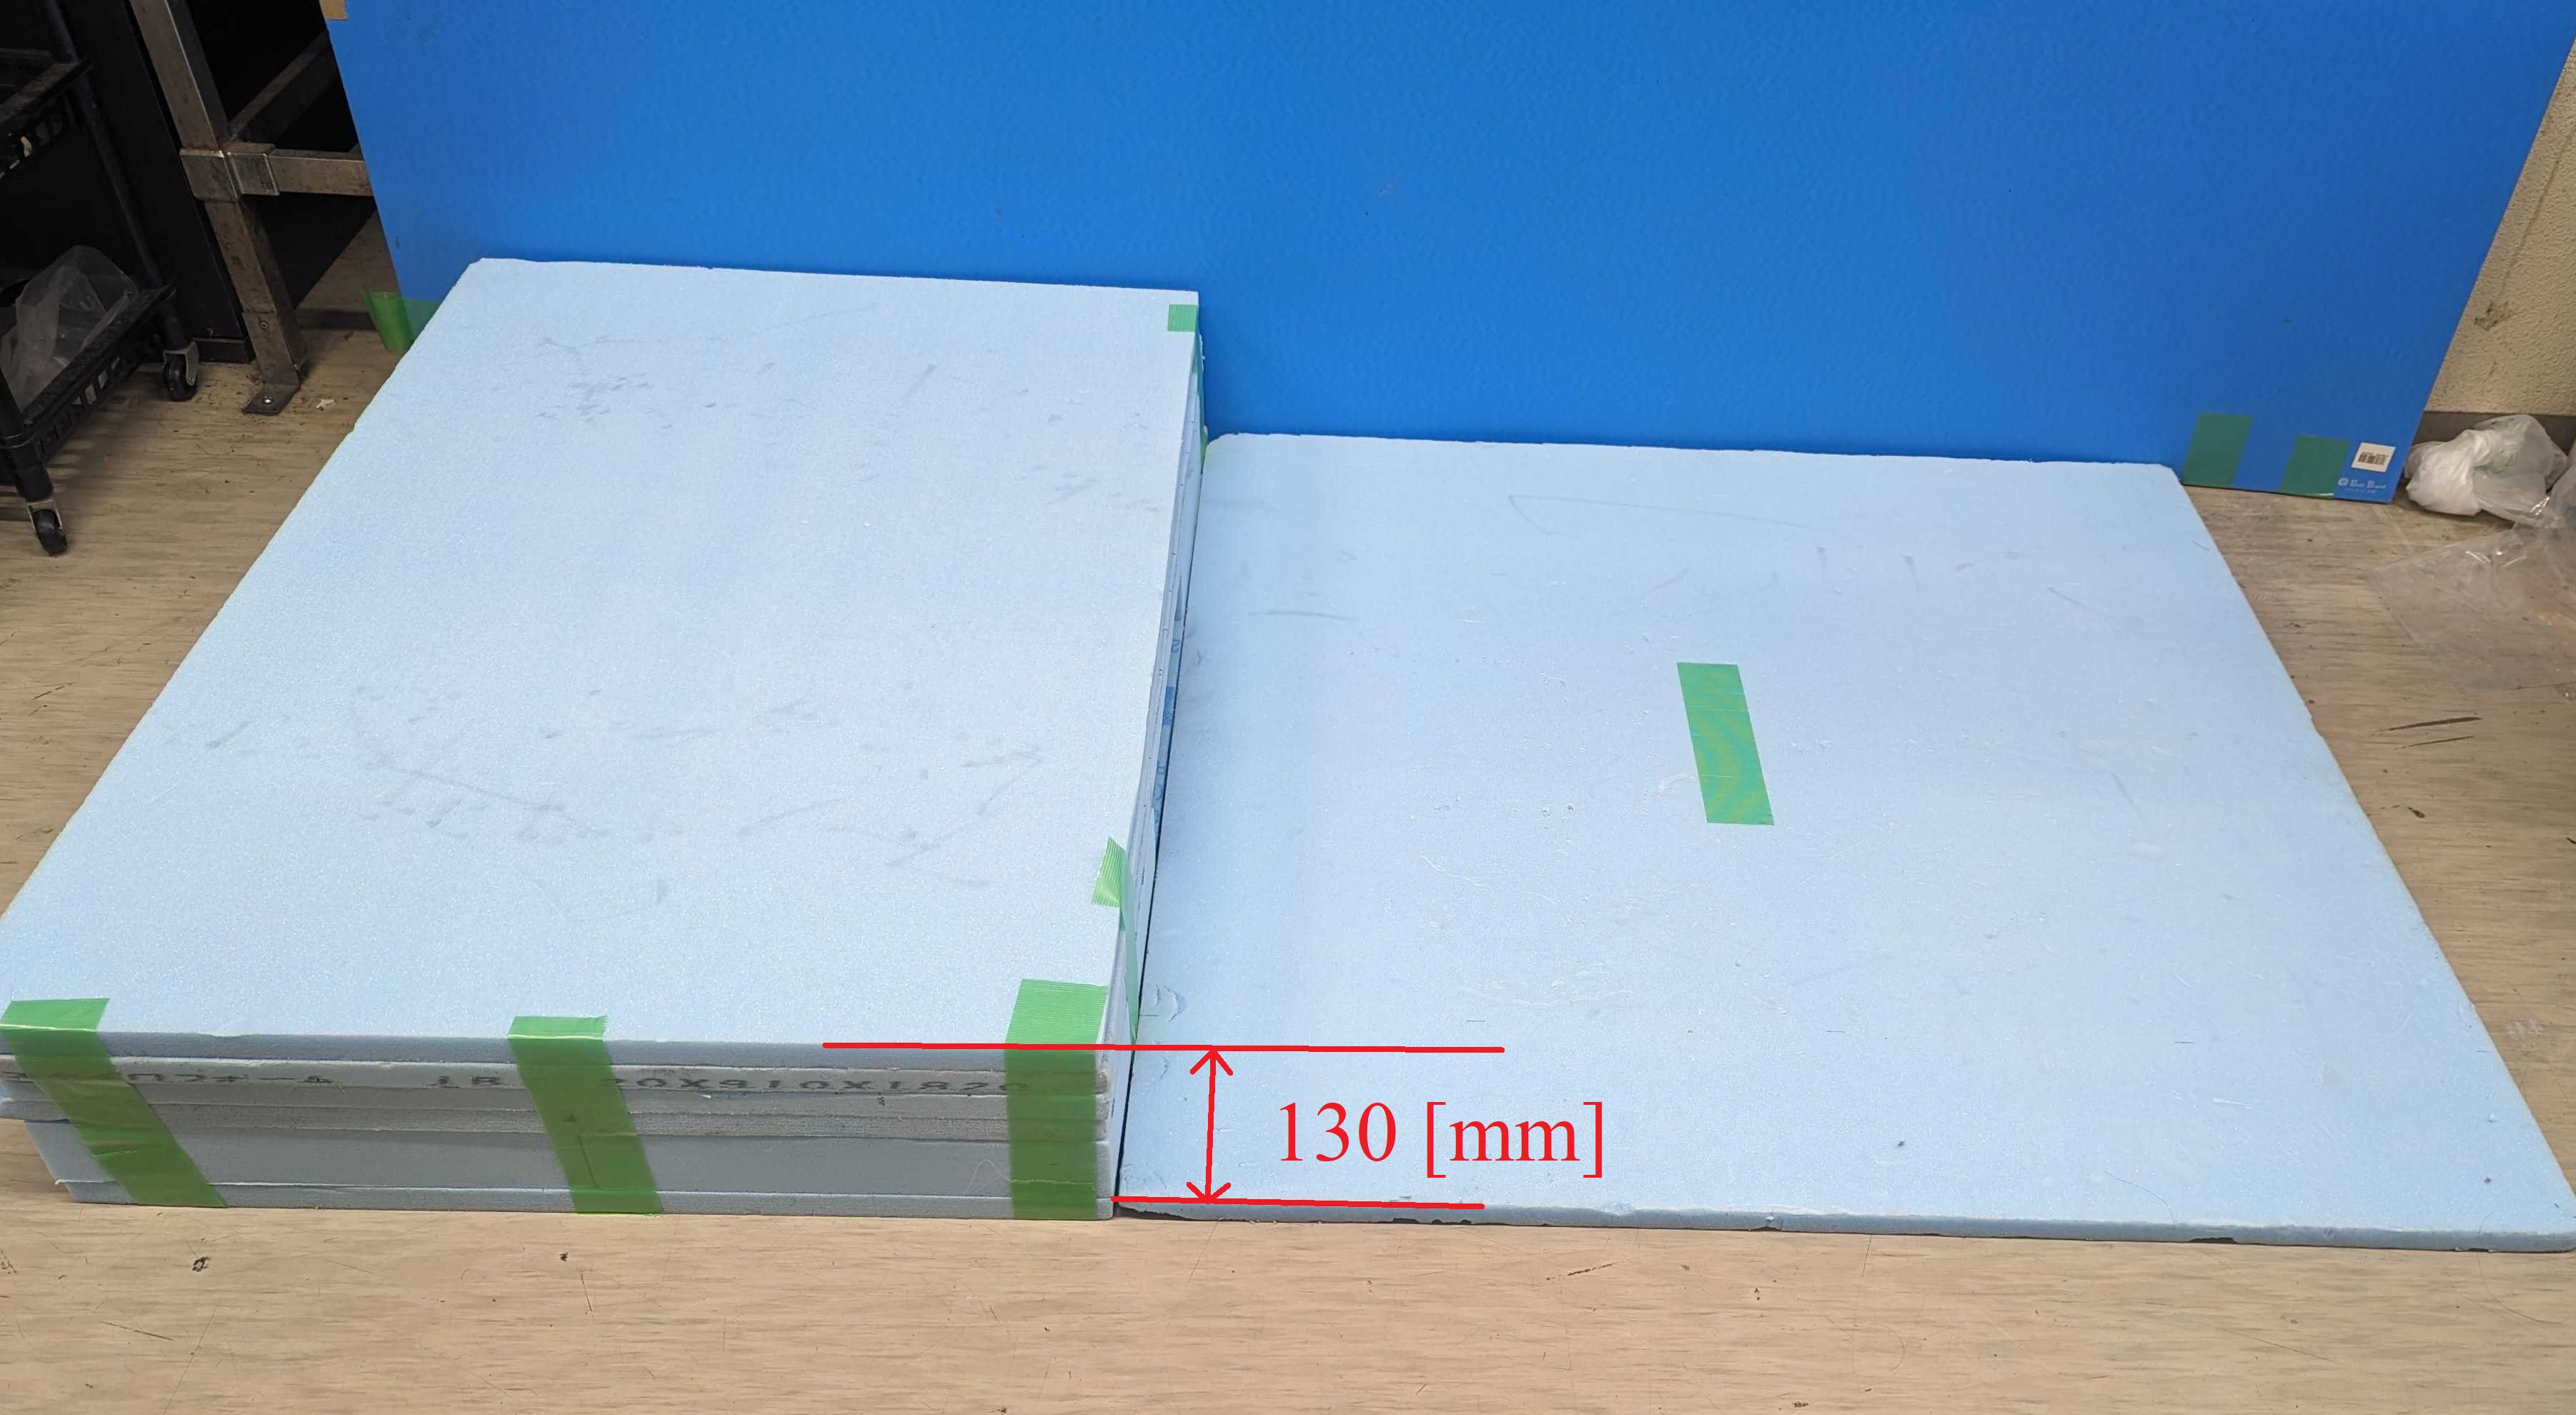
\includegraphics[width=0.8\linewidth]{figure/chapter5/walking-terrain.jpg}
  \caption{Walking Terrain}
  \label{fig:walking-terrain}  % chktex 24
\end{figure}

\subsection{使用したロボット}
実験ではシミュレーションのモデルとしていたPhantomXを使用した.
内部電源では長時間稼働させるには容量が足りないため,
電源には外部電源として安定化電源($12V,5A$)を使用した.
ロボットへの指令値は,グラフ探索による自由歩容パターン生成手法を用いてPCで計算し,
XBeeを用いてPhantomXに送信した.

ロボットの脚軌道は矩形軌道を用いた.
また,本実験は先行研究では歩行ができなかった地形で歩行ができることを示すことが目的であるため,
地形は既知のものとし,地形の形状をセンサで計測することは行わなかった.

\subsection{実験の条件}
歩行実験時の歩行条件を以下に示す.

\begin{itemize}
  \item 胴体姿勢は常に地面と水平にする
  \item 動作は直進動作のみを行う
  \item ロボットの重心からみた遊脚高さは-20mmとする
  \item 安定余裕を15mmとする
  \item 胴体は地形から30mm以上離す
\end{itemize}

また,グラフ探索の条件を以下に示す.

\begin{itemize}
  \item 探索するグラフの深さは5とする
  \item 近似された可動範囲の最小半径は140mmとする
\end{itemize}

\subsection{実験の手順}
まず,ロボットを段差の手前に配置した.
次に,130mmの段差を上りおよび下りするまでの自由歩容パターンを生成し,
ロボットにXBeeを通じて送信した.
そして,送信された指令値に基づいてロボットが歩行する様子を撮影した.
ロボットの6脚すべてが段差を乗り越えることができた場合に,
ロボットが段差を乗り越えたと判断した.

\section{結果}
130mmの段差を歩行する様子を\figref{fig:ch5_experiment_1}に示す.
この図は,ロボットが動作する様子をタイムラプスで撮影したものである.
30枚の写真で構成されており,初めから順番に01から30までの番号が右上に振られている.
この図から,ロボットが重心高さを変更し130mmの段差を上る様子が確認できる.
ロボットは最初,画面右側に配置され,胴体高さを上げたのち,
段差の上に脚を接地して段差を上り,画面左側に向けて歩行している.

130mmの段差を下りる様子を\figref{fig:ch5_experiment_2}に示す.
この図も同様にタイムラプスで撮影している.
この図から,ロボットが重心高さを変更し130mmの段差を下る様子が確認できる.
ロボットは最初,画面左側に配置され,段差の下へ胴体を乗り出しつつ脚を接地し,
段差を下ったのち胴体高さを下げて,画面右側に向けて歩行している.

\begin{figure}[tb]
  \centering
  \includegraphics[width=0.7\linewidth]{figure/chapter5/up.png}
  \caption{Actual Equipment Experiment (130mm steps up)}
  \label{fig:ch5_experiment_1}  % chktex 24
\end{figure}

\begin{figure}[tb]
  \centering
  \includegraphics[width=0.7\linewidth]{figure/chapter5/down.png}
  \caption{Actual Equipment Experiment (130mm steps down)}
  \label{fig:ch5_experiment_2}  % chktex 24
\end{figure}

\section{考察} % 第5章
		

\chapter{結論}\label{chapter:結論}

\section{結論}

本論文では,まずグラフ探索による自由歩容パターン生成手法の先行研究の問題点を指摘し,
その問題点を解決するための歩容パターンの再評価手法を提案した.
次に再評価手法の実装方法を述べ,実装した再評価手法を用いてシミュレーション実験を行いその結果を示した.
そして,シミュレーションの結果より本問題において再評価手法は有効でないことと,
近似された可動範囲における,最小半径の変更によって先行研究の問題点を解決できることを示した.

第1章「序論」では,グラフ探索による自由歩容パターン生成手法の利点を示し,
同時に先行研究で確認された脚軌道生成の失敗を述べた.

第2章「歩容パターンの再評価手法の提案」では,
シミュレーション実験によって脚軌道生成の失敗を確認し,
脚軌道生成失敗を防ぐ手段として再評価手法を提案した.

第3章「歩容パターンの再評価手法の実装」では,
2章で述べた再評価手法の実装方法を述べた.

第4章「再評価手法の有効性の確認のための歩行シミュレーション」では,
実装した再評価手法を用いたシミュレーション実験の結果を示し,
最小半径を140mmに設定した場合,脚軌道生成の失敗が生じずに歩行することが可能であることを示した.
また,再評価手法は本問題に対しては有効でないことを示した.

第5章「常に脚軌道生成が可能な自由歩容パターン生成手法を用いた実機実験」では
最小半径を140mmに設定し,先行研究では歩行することができなかった地形で実機を用いて歩行実験を行った.
その結果,先行研究では歩行することができなかった地形であっても歩行することができることを確認し,
脚軌道生成の失敗による動作停止を防ぐことができたことを示した.

\section{今後の展望}
本研究が取り扱った問題については,再評価手法は適切な手法ではないことが示されたが,
他の問題については再評価手法は有効である可能性がある.
具体的にはトルク不足による脚の沈み込みである.
グラフ探索の処理では計算時間を短縮するために,
力学的な計算を行っていない.
しかしそれを原因として,実機実験時にトルク不足による脚の沈み込みが生じてしまうことが確認されている.
そこで,グラフ探索によって得られた歩容パターンを実機で実行する前に,
力学的な計算を用いてトルクが不足していないかを確認し,
トルク不足が生じている場合は再評価手法を用いて歩容パターンを再評価することで,
トルク不足による脚の沈み込みを防ぐことができると考えられる.

 % 第6章
    %%%%%%%%%%%%%%%%%%%%%%%%%%%%%%%%%%%%%%%%%%%%%%%%%%%%%%%%%%%%%%%%%%%%%%%%
%%
%% 付録.tex
%% LaTeX-2e 専用
%% 
%% 
%%        設計工学研究室 学位論文テンプレート
%%
%%                      作成日時    2010年 12月 17日
%%
%%%%%%%%%%%%%%%%%%%%%%%%%%%%%%%%%%%%%%%%%%%%%%%%%%%%%%%%%%%%%%%%%%%%%%%%

\appendix
%%%%%%%%%%%%%%%%%%%%%%%%%%%%%%%%%%%%%%%%%%%%%%%%%%%%%%%%%%%%%%%%%%%%%%%%
%%
%% 付録.tex
%% LaTeX-2e 専用
%% 
%% 
%%        設計工学研究室 学位論文テンプレート
%%
%%                      作成日時    2010年 12月 17日
%%
%%%%%%%%%%%%%%%%%%%%%%%%%%%%%%%%%%%%%%%%%%%%%%%%%%%%%%%%%%%%%%%%%%%%%%%%

\chapter{C++20への移行}\label{chapter:付録A}
\section{C++20の新機能}
C++にはコンパイラの標準規格として,C++98,C++03,C++11などが存在する.
その中でもC++11以降は約3年に一度のペースで新しい規格が策定されている.
先行研究のプログラムでは,C++17を使用していたが,本研究ではC++20\cite{Thomas_C++20}を使用するように変更を行った.
C++20では,C++17からの変更点として,以下のようなものがある.
\begin{itemize}
  \item constexpr関数の制限緩和
  \item 標準ライブラリの多くの関数がconstexpr関数に変更
  \item conceptの導入
  \item std::number,std::formatの導入
\end{itemize}
これらの機能を使用することで,プログラムの最適化を行うことができる上,可読性を向上されることができる.
以下に各機能の詳細を記述する.

\section{constexpr変数・関数}
constexpr関数はコンパイル時に評価される関数であり,
C言語におけるマクロ関数のような処理を実現するために使用される.
たとえば,以下のようなプログラムを考える.

\newpage  % 改ページする

\begin{lstlisting}[caption=convert func as macro,label=convert_func_as_macro]
#include <iostream>

// defined as macro
#define CONVERT_TO_RAD(deg) (deg * 3.1415926535f / 180.0f)  

int main()
{
  float deg = 90.0f;
  
  // It will deploy deg * 3.1415926535f / 180.0f.
  std::cout << CONVERT_TO_RAD(deg) << std::endl;
}
\end{lstlisting}

% 1行開ける
\vskip \baselineskip

このプログラムでは,マクロ関数を使用して,度数法で表された角度をラジアンに変換している.
プログラムを記述する際にはラジアンで角度を表現すると可読性が低くなるため,
度数法で記述することによる利点は大きいが,実際の処理ではラジアンで角度を表現する必要があるので,
このようなマクロが実際に使用されることは多いだろう.

しかし,マクロにはいくつかの問題点がある.
まず1つとして,マクロは常にグローバルスコープで定義されることである.
通常C++の開発においては,クラスや名前空間を使用して,変数や関数をスコープを限定して定義することが多い.
スコープを限定することは,変数や関数の名前が衝突することを防ぐことができるため,
大規模な開発や複数のライブラリを使用する場合には必須である.
だが,マクロは名前空間内に定義したとしてもグローバルスコープに展開されるため,
名前の衝突を防ぐことができないのである.

もう1つの問題点は,マクロは型の確認を行わないことである.
C++はpythonやjava scriptなどの動的型付け言語とは異なり静的型付け言語である.
そのため,コンパイル時に型の不一致や意図しないキャストを警告として出力することができ,
ランタイムエラーを防ぐことができる.
しかし,マクロはプリコンパイル時に文字を置換するだけであるため,型の確認を行わない.
そのためたとえば上記のマクロ関数において,引数をint型やdouble型,果てはその他のクラスなどに変更しても,
float型との掛け算演算子が定義されていればコンパイルは通ってしまう.
先行研究のプログラムではマクロ関数を使用している箇所が多く存在したため,
実際に浮動小数点型のfloat型とdouble型が混在している箇所が存在した.

これをconstexpr関数を使用することで,以下のように書き換えることができる.

\newpage  % 改ページする

\begin{lstlisting}[caption=convert func as constexpr,label=convert_func_as_constexpr]
#include <iostream>

// defined as constexpr function
constexpr float ConvertToRad(float deg)
{
  return deg * 3.1415926535f / 180.0f;
}

int main()
{
  // declared as constexpr variable
  constexpr float deg = 90.0f;
  
  // It will deploy 1.57079632675f.
  std::cout << ConvertToRad(deg) << std::endl;
}
\end{lstlisting}

% 1行開ける
\vskip \baselineskip

このようにconstexpr関数を使用することで,マクロ関数のようにコンパイル時に評価される関数を定義することができる.
また,constexpr関数はコンパイル時に評価が行われるため,コンパイル時に型の確認を行うことができる.
加えて,constexpr関数はスコープを限定することができるため,名前の衝突を防ぐことができる.

以上のようにマクロの持つ問題点を解決することができるが,constexpr関数の本当の利点はコンパイル時に処理が実行されることである.
\ref{convert_func_as_constexpr}の14,15行目にあるように,引数を含めてコンパイル時に評価が可能であれば,
コンパイル時に関数が実行される.そのため,関数の呼び出しによるオーバーヘッドを削減することができる.



\chapter{PhantomX Mark I\hspace{-1.2pt}Iのサーボモータ}\label{chapter:B}
\section{サーボモータの仕様}

PhantomX Mark I\hspace{-1.2pt}Iは計18個のサーボモータを搭載しており,
Dynamixel AX-12A,あるいはDynamixel AX-18Aを搭載したモデルがある.
今回使用したのはDynamixel AX-18Aを搭載したモデルであるため,
以下にDynamixel AX-18Aの仕様をまとめたWebページを掲載する.
(https://e-shop.robotis.co.jp/product.php?id=235 アクセス日 2023/9/15)

\begin{figure}
  \centering
  \begin{tabular}{cc}
    \fbox{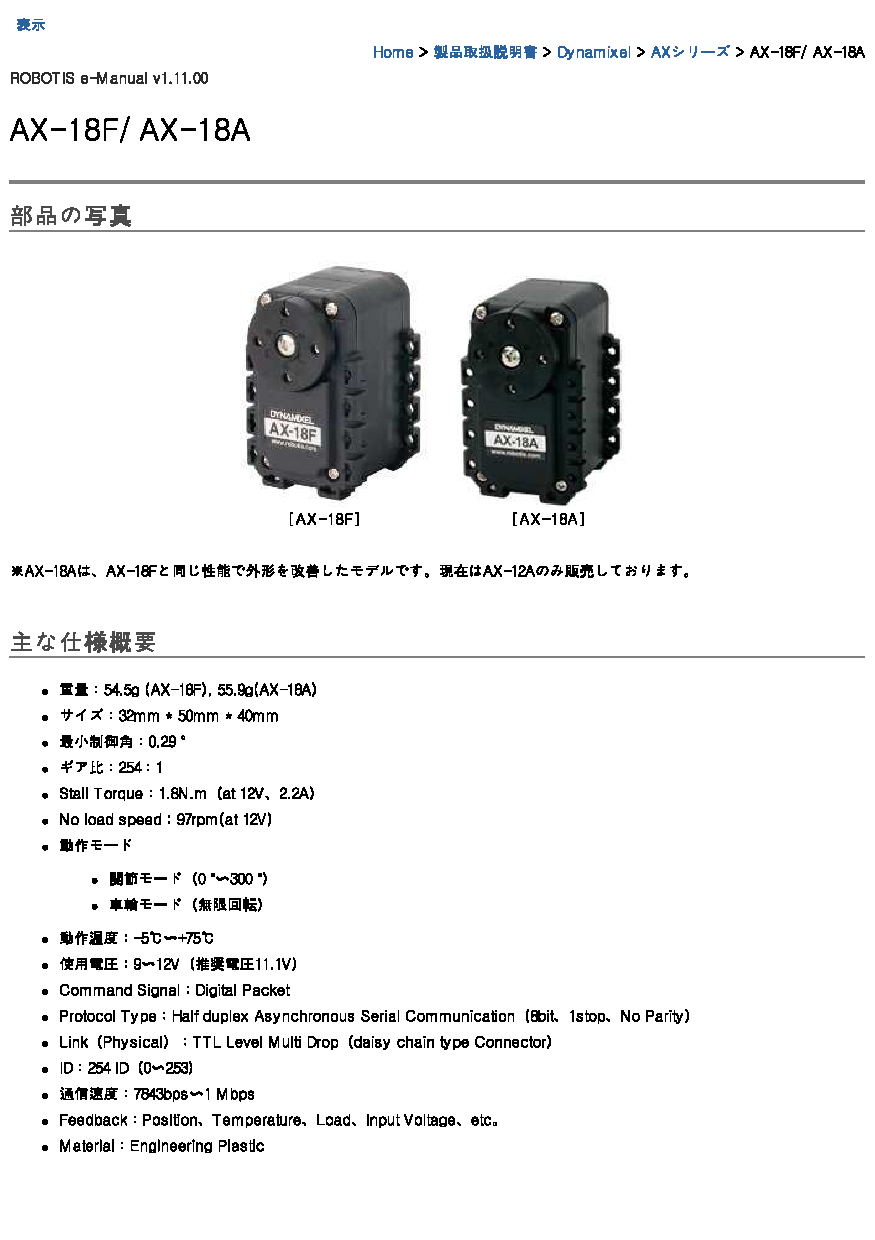
\includegraphics[page=1, width=0.4\textwidth]{web_page/AX-18A_Manual.pdf}} &
    \fbox{\includegraphics[page=2, width=0.4\textwidth]{web_page/AX-18A_Manual.pdf}} \\
    Page 1 & Page 2 \\
  \end{tabular}

  \caption{Dscription AX-18A (page1--2)}
  \label{fig:ax-18_1-2}  % chktex 24
\end{figure}

\begin{figure}
  \centering
  \begin{tabular}{cc}
    \fbox{\includegraphics[page=3, width=0.4\textwidth]{web_page/AX-18A_Manual.pdf}} &
    \fbox{\includegraphics[page=4, width=0.4\textwidth]{web_page/AX-18A_Manual.pdf}} \\
    Page 3 & Page 4 \\
    \fbox{\includegraphics[page=5, width=0.4\textwidth]{web_page/AX-18A_Manual.pdf}} &
    \fbox{\includegraphics[page=6, width=0.4\textwidth]{web_page/AX-18A_Manual.pdf}} \\
    Page 5 & Page 6 \\
  \end{tabular}

  \caption{Dscription AX-18A (page3--6)}
  \label{fig:ax-18_3-6}  % chktex 24
\end{figure}

\begin{figure}
  \centering
  \begin{tabular}{cc}
    \fbox{\includegraphics[page=7, width=0.4\textwidth]{web_page/AX-18A_Manual.pdf}} &
    \fbox{\includegraphics[page=8, width=0.4\textwidth]{web_page/AX-18A_Manual.pdf}} \\
    Page 7 & Page 8 \\
    \fbox{\includegraphics[page=9, width=0.4\textwidth]{web_page/AX-18A_Manual.pdf}} &
    \fbox{\includegraphics[page=10, width=0.4\textwidth]{web_page/AX-18A_Manual.pdf}} \\
    Page 9 & Page 10 \\
  \end{tabular}

  \caption{Dscription AX-18A (page7--10)}
  \label{fig:ax-18_7-10}  % chktex 24
\end{figure}

\begin{figure}
  \centering
  \begin{tabular}{cc}
    \fbox{\includegraphics[page=11, width=0.4\textwidth]{web_page/AX-18A_Manual.pdf}} &
    \fbox{\includegraphics[page=12, width=0.4\textwidth]{web_page/AX-18A_Manual.pdf}} \\
    Page 11 & Page 12 \\
    \fbox{\includegraphics[page=13, width=0.4\textwidth]{web_page/AX-18A_Manual.pdf}} & 
    \\
    Page 13 &  \\
  \end{tabular}

  \caption{Dscription AX-18A (page11--13)}
  \label{fig:ax-18_11-13}  % chktex 24
\end{figure}

% 改ページする
\clearpage
 

% \section{計算手順}

% \chapter{脚機構図面}\label{chapter:付録B}
% \section{組図}
% \section{断面図}
                                          %付録(あれば)
    \backmatter{}                                                %章番号を付けない
    
\chapter*{謝辞}\label{chapter:謝辞}
\addcontentsline{toc}{chapter}{謝辞}

本論文の研究と執筆にあたりその細部に至るまで終始懇切なる御指導と御鞭撻を賜りました,
埼玉大学大学院理工学研究科琴坂信哉准教授,程島竜一准教授に謹んで深謝の意を申し上げます.

また,研究室において常に熱心な御討論を頂きました,OB・学生の方々に感謝の意を表します.
                                          %謝辞
    \begin{thebibliography}{99}
    \bibitem{Sotnik_Prospects_for_Introduction}
    Sotnik S, Lyashenko V:
    ``Prospects for Introduction of Robotics in Service'',
    International Journal of Academic Engineering Research.
    Vol.6,
    pp.4-9, % chktex 8
    2022.

    \bibitem{Pudu_BellaBot}
    Pudu Robotics Inc:
    ``BellaBot'',
    https://www.pudurobotics.com/jp/products/bellabot (参照2024/01/23).

    \bibitem{Locomotion_for_difficult_terrain}
    Freyr Hardarson:
    ``Locomotion for difficult terrain'',
    1997.

    \bibitem{Boston_Dynamics_Spot}
    Boston Dynamics Inc:
    ``Spot®'',
    https://bostondynamics.com/products/spot/ (参照2024/01/23).

    \bibitem{NEDO}
    国立研究開発法人 新エネルギー・産業技術総合開発機構:
    ``NEDO 先導研究プログラム 2021年度'',
    Vol.1,
    p.57, 
    2022. 

    \bibitem{J_Kim_Dexterous_Crabster}
    B. H. Jun, Hyungwon Shim:
    ``A Dexterous Crabster Robot Explores the Seafloor'',
    The ACM Magazine for Students,
    Vol.20,
    pp.38--45,
    2014.

    \bibitem{J_Kim_Little_Crabster}
    J. Y. Kim, B. H. Jun:
    ``Mechanical Design of Six-Legged Walking Robot, Little Crabster'',
    Oceans-Yeosu,
    pp.1--8,
    2012.

    \bibitem{Hirose_Static_stability_criterion}
    広瀬,塚越,米田: 
    ``不整地における歩行機械の静的安定性評価基準'', 
    J. of Robotic Systems,
    Vol.16, No.8, 
    pp.1076--1082,
    1998.

    \bibitem{Prabir_Graph_search}
    Prabir K. Pal, K. Jayarajan: 
    ``Generation of Free Gait A Graph Search Approach'',
    IEEE Transactions on Robotics and Automation,
    Vol.7, No.3,
    1991.

    \bibitem{Prabir_Graph_search_Six}
    Prabir K. Pal, V. Mahadev and K. Jayarajan:
    ``Gait generation for a six-legged walking machine through graph search'',
    Proceedings of the 1994 IEEE International Conference on Robotics and Automation,
    vol.2,
    pp.1332--1337,
    1994.

    \bibitem{Arata_Graph_search_Six}
    新, 田窪, 上野:
    ``障害物環境下におけるトライポッド歩容の脚配置計画'',
    ロボティクス・メカトロニクス講演会講演概要集,
    2015.

    \bibitem{Oki_Graph_search}
    大木,程嶋,琴坂: 
    ``多脚ロボットの不整地踏破を目標とするグラフ探索を用いた歩行パターン生成'', 
    ロボティクス・メカトロニクス講演会講演概要集,
    2015.   

    \bibitem{Nakaoka_Graph_search}
    中岡,程嶋,琴坂: 
    ``不整地における特定位置・脚着地点への遷移を目的とした多脚歩行ロボットの歩行動作計画'',
    日本機械学会関東支部総会講演会講演論文集,
    2016.

    \bibitem{Shina_Graph_search}
    椎名,程嶋,琴坂: 
    ``グラフ探索を用いた多脚ロボットの旋回歩容パターン生成'',
    日本機械学会関東支部総会講演会講演論文集,
    2018.

    \bibitem{Miura_Graph_search}
    三浦,程嶋,琴坂: 
    ``グラフ探索による多脚歩行ロボットの自由歩容パターン生成 第4報:出現頻度によるノード枝刈りを用いた探索時間の短縮'',
    日本機械学会関東支部総会講演会講演論文集,
    2019.

    \bibitem{Hato_Graph_search}
    波東,程嶋,琴坂: 
    ``グラフ探索による多脚歩行ロボットの自由歩容パターン生成 第5報: 重心の上下移動のエッジを用いた重心高さの変更'',
    日本機械学会関東支部総会講演会講演論文集,
    2020.

    \bibitem{Program_Challenge_Book}
    秋葉, 岩田, 北川:
    ``プログラミングコンテストチャレンジブック'',
    毎日コミュニケーションズ,
    2010.
    
    \bibitem{Dxlib_Web}
    DXライブラリ置き場.
    https://dxlib.xsrv.jp/ (参照2024/01/23).

    \bibitem{cita:phantom_x_mark_2}
    Trossen~Robotics:
    ``PhantomX~AX~Hexapod~Mark~II~Kit''.
    \url{https://www.trossenrobotics.com/hex-mk2},
    (参照2024/01/23).

    \bibitem{Thomas_C++20}
    Thomas~Koppe:
    ``Changes~between~C++17~and~C++20~DIS''.
    \url{https://www.open-std.org/jtc1/sc22/wg21/docs/papers/2020/p2131r0.html}, 
    (参照2024/01/23).

    \bibitem{cita:ax_18a_manual}
    ROBOTIS:
    ``AX-18A~User~Manual''.
    \url{https://e-shop.robotis.co.jp/product.php?id=235},
    (参照2023/9/15).

\end{thebibliography}
\endinput                                 %参考文献
\end{document}